\documentclass[times, utf8, diplomski]{fer}
\usepackage{booktabs}
\usepackage{color}
\usepackage{listings}
\usepackage{pdfpages}
\usepackage{subcaption}
\usepackage{float}
\usepackage{enumitem}

\graphicspath{ {./resources/images/} }
\renewcommand{\lstlistingname}{K\^{o}d}%
\lstset{ %
language=C++,                % choose the language of the code
basicstyle=\footnotesize,       % the size of the fonts that are used for the code
numbers=left,                   % where to put the line-numbers
numberstyle=\footnotesize,      % the size of the fonts that are used for the line-numbers
stepnumber=1,                   % the step between two line-numbers. If it is 1 each line will be numbered
numbersep=5pt,                  % how far the line-numbers are from the code
backgroundcolor=\color{white},  % choose the background color. You must add \usepackage{color}
showspaces=false,               % show spaces adding particular underscores
showstringspaces=false,         % underline spaces within strings
showtabs=false,                 % show tabs within strings adding particular underscores
frame=single,           % adds a frame around the code
tabsize=2,          % sets default tabsize to 2 spaces
captionpos=b,           % sets the caption-position to bottom
breaklines=true,        % sets automatic line breaking
breakatwhitespace=false,    % sets if automatic breaks should only happen at whitespace
escapeinside={\%*}{*)}          % if you want to add a comment within your code
}

\setlist[enumerate]{%                
labelindent=\parindent,%  
leftmargin=*,%                          
listparindent=-\leftmargin% 
}

\begin{document}

% TODO: Navedite broj rada.
\thesisnumber{2926}

% TODO: Navedite naslov rada.
\title{3D interaktivna vizualizacija simulacije vibracija}

\author{Nikola Vugdelija}

\maketitle

% Ispis stranice s napomenom o umetanju izvornika rada.
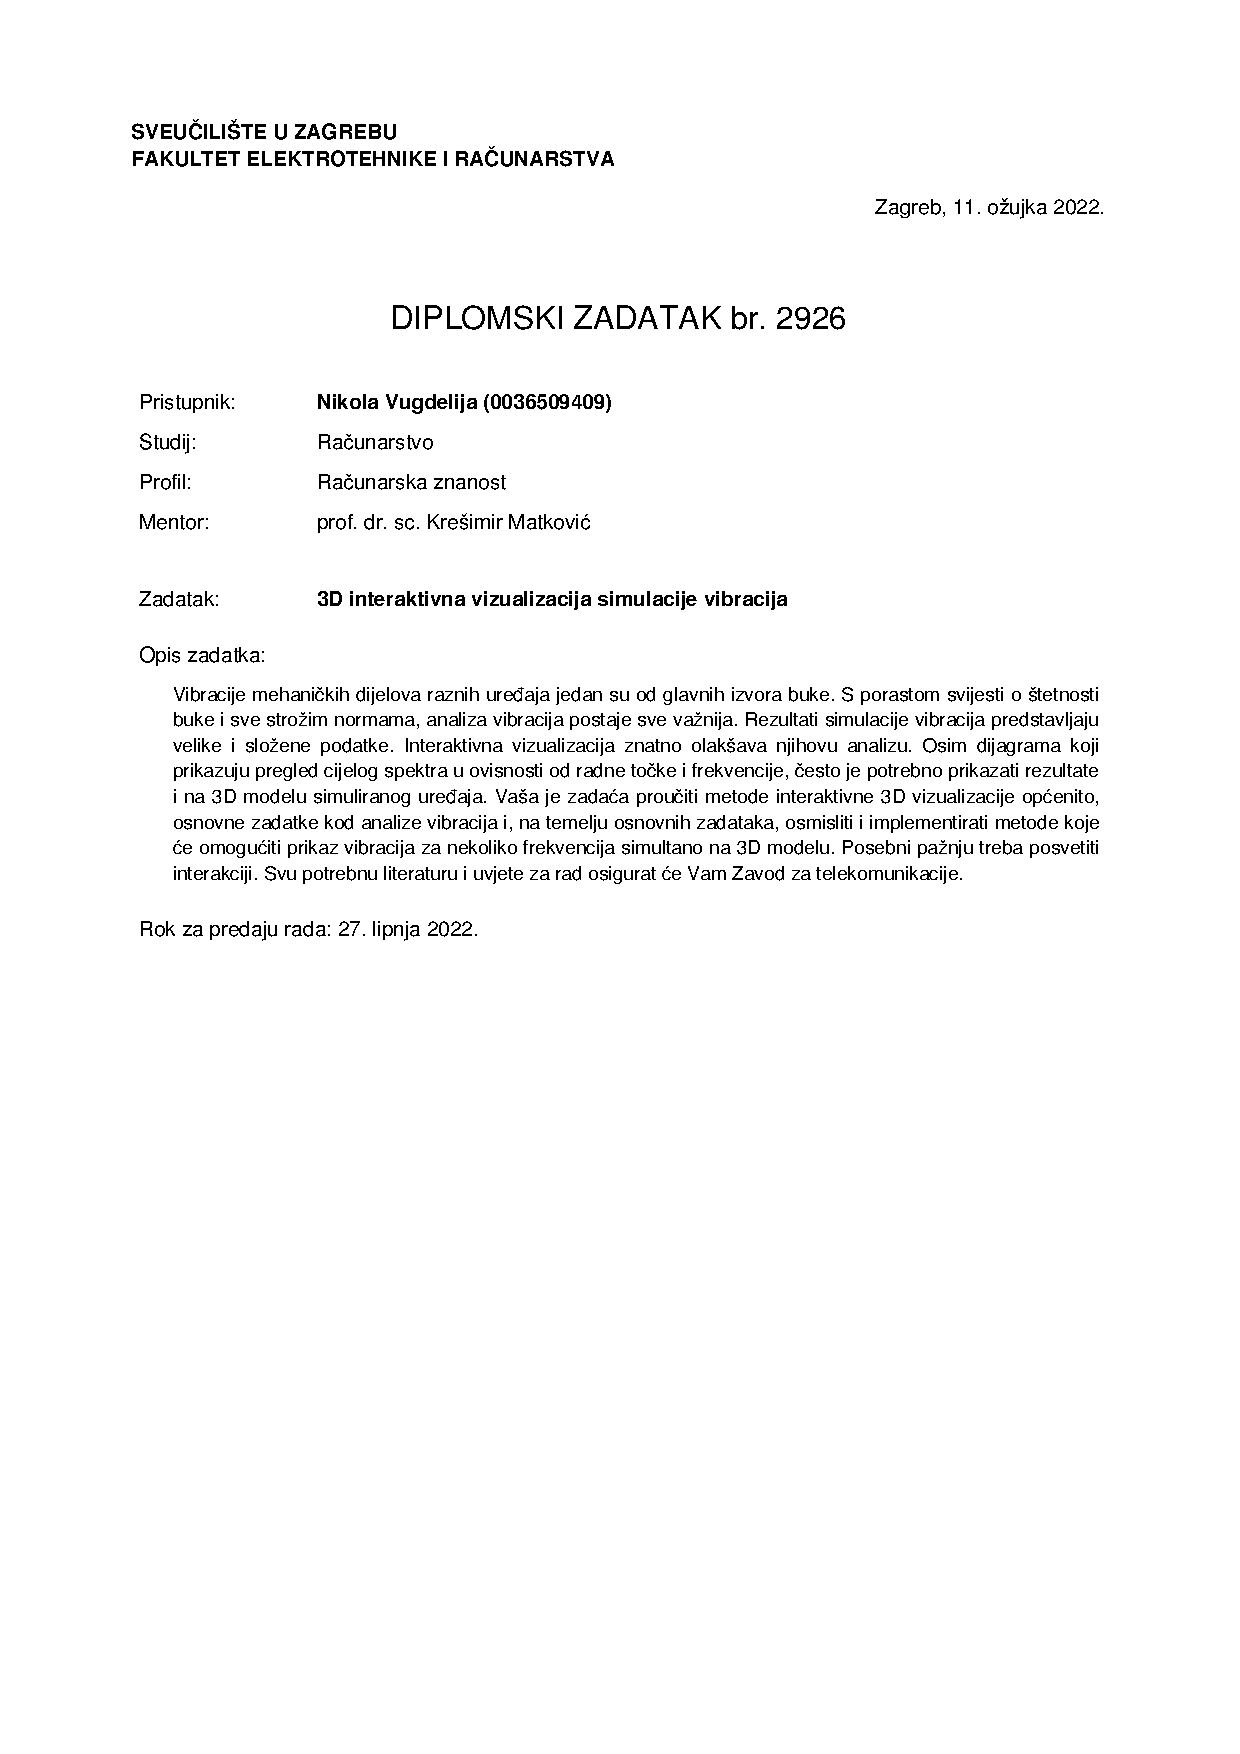
\includepdf[pages=-]{resources/docs/task.pdf}


% Dodavanje zahvale ili prazne stranice. Ako ne želite dodati zahvalu, naredbu ostavite radi prazne stranice.
\zahvala{Zahvaljujem se mentoru prof. dr. sc. Krešimiru Matkoviću na velikoj pomoći pri pisanju ovog rada. Hvala mojim roditeljima na svemu što su mi omogućili, te hvala svim bližnjima na pruženoj podršci. Konačno, hvala dragom Bogu na svemu što mi je podario.}

\tableofcontents

\listoffigures

\chapter{Uvod}
Buka i vibriranje motora su jedni od ključnih faktora koji utječu na osjećaj udobnosti putnika u osobnom automobilu. No, iako se može reći kako je osjećaj udobnosti subjektivne prirode, propisi koji kontroliraju dozvoljene razine buke koju u okolišu proizvodi motor vozila su objektivni i egzaktni. Dva osnovna izvora buke su strujanje zraka i mehaničke vibracije, pa ih zbog navedenih razloga inženjeri nastoje održati na što nižoj razini prilikom rada. Ovaj rad se fokusira na mehaničke vibracije, a NVH \engl{Noise, Vibration, Harshness} simulacije predstavljaju najjednostavniji način njihovog analiziranja u fazi projektiranja motora. Termin NVH u automobilskoj industriji označava podatke koji pomažu u suzbijanju buke, dizajnu buke te suzbijanju vibracije, cviljenja i zveckanja motora \citep{harrison2004vehicle}. NVH simulacije inženjerima omogućuju precizan uvid u razinu vibriranja pojedinih dijelova motora, stoga probleme koji uzrokuju nepoželjno vibriranje dijelova motora mogu riješiti tijekom projektiranja.\\

No, računanje simulacije je samo dio problema. Matković et al. \citep{matkovic2021getting} tvrde kako računske simulacije ove vrste, nerijetko proizvode podatke koje se ne može jednostavno vizualizirati i analizirati. Iz tog razloga je potrebno podatke prikazati intuitivno i razumljivo kako bi ih stručnjaci mogli koristiti na što efikasniji način. Iako su podaci prikazani u obliku tablica i grafova korisni, vizualizacijom istih podataka na 3D modelu motora se postiže jasniji, intuitivniji i potpuniji prikaz potencijalnih izvora buke.\\

Ovaj rad opisuje izradu alata za vizualizaciju podataka dobivenih iz NVH simulacije pomoću 3D modela motora i 2D grafova. Fokus predstavljenog alata je na vizualizaciji snage vibracije dijelova motora na višestrukim frekvencijama vibriranja motora, kako bi se razine vibracije različitih taktova motora jednostavnije uspoređivale.

\chapter{Pregled područja} \label{area-overview-section}
Vizualizacija podataka je iznimno važno područje analize podataka. Budući da isti skup podataka može prenijeti potpuno drugačije informacije ovisno o načinu prikaza, od velike je važnosti odabrati optimalne vizualizacijske tehnike za konkretni skup podataka. Unwin \citep{Unwin2020Why} naglašava kako kod vizualizacije ne postoji jedna "optimalna" grafika koja najbolje prikazuje svaki skup podataka, nego je često potrebno pronaći grupu vizualizacijskih tehnika koje se međusobno upotpunjuju i prikazuju cjelovitu sliku. Stoga je tijekom osmišljavanja alata za vizualizaciju izrazito važno utvrditi za koju svrhu se taj alat koristi, te koje informacije je potrebno njime vizualizirati iz danog skupa podataka. Odgovori na navedena pitanja postaju kompleksniji za odgonetnuti s porastom kompleksnosti skupa podataka koji alat vizualizira. Zbog toga je pomoć stručnjaka u domeni itekako korisna.\\

Kao što je već spomenuto, glavna svrha alata razvijenog u sklopu ovog rada je vizualizacija NVH podataka na modelu motora. Prilikom izrade ovog rada je korišten isti skup podataka koji je korišten prilikom izrade alata u sklopu rada Matkovića et al.\citep{matkovic2021getting}. Spomenuti podaci su izračunati NVH simulacijom pomoću alata AVL EXCITE™ \citep{avlEXCITE}. Motor je zadan kao skup konačnih elemenata, a za svaki element su poznate koordinate vrhova u 3D prostoru, te kojom snagom element vibrira pri različitim frekvencijama vibracije motora. Skup podataka također definira i ograničenja koja ljestvicu snage vibriranja elemenata dijele na tri dijela (bezopasni, rizični i opasni) pomoću dva faktora. Navedeni dijelovi su bazirani na razini buke koju element proizvodi vibriranjem tom snagom pri zadanoj frekvenciji.\\

Stručnjake pri analizi NVH podataka ponajprije zanimaju tri stavke \citep{matkovic2021getting}:

\begin{itemize}
\item Usporedba snage vibriranja motora na različitim frekvencijama vibracije motora
	\begin{itemize}
	\item Kako se snaga vibracije mijenja na pojedinim dijelovima motora s promjenom frekvencije vibracije motora?
	\end{itemize} 
\item Lokalizacija značajki
	\begin{itemize}
	\item Koji elementi motora vibriraju snagom koja pripada zadanom rasponu?
	\end{itemize} 
\item Lokalna pretraga
	\begin{itemize}
	\item Kojom snagom vibriraju odabrani elementi?\\
	\end{itemize} 
\end{itemize}

Alat razvijen u sklopu referiranog rada dobro adresira navedene značajke. Koristeći paralelne koordinate \citep{inselberg1990}, omogućen je detaljan pregled usporedbe podataka na različitim frekvencijama vibracije motora. Adresiranje druge i treće značajke je olakšano korištenjem višestrukih, međusobno povezanih prozora s 3D prikazom motora. Lokalna pretraga je ostvarena uz pomoć interaktivne selekcije koju korisnik može koristiti za biranje raspona snage vibracije za određene frekvencije, a svi prozori automatski ažuriraju prikaz modela motora označujući elemente koji pripadaju zadanim rasponima. Konačno, Matković et al. \citep{matkovic2021getting} su lokalnu pretragu omogućili bojanjem modela motora bazirano na snazi vibracije pojedinačnih elemenata pri zadanoj frekvenciji vibriranja motora. Detaljniji uvid u snagu vibriranja pojedinih elemenata modela je omogućen odabirom interesnog elementa, nakon čega se istakne 2D graf vibracija tog elementa.\\

No, iako je referirani rad cjelokupno odlično pokrio sve tri značajke, u području usporedbe snage vibracije dijelova motora na različitim frekvencijama vibracije još ima prostora za napredak. Naime, trenutna usporedba podataka na različitim frekvencijama je moguća samo pomoću 2D grafova koji, iako su korisni, imaju problema s čitljivošću i jasnoćom. Alat koji je razvijen u sklopu ovog rada implementira niz vizualizacijskih tehnika, sa fokusom na 3D vizualizaciju, koje potencijalno povećavaju intuitivnost usporedbe vibracija dijelova motora na različitim frekvencijama vibriranja u odnosu na izvedbu kod alata iz referiranog rada.

\chapter{Analiza zadatka i zahtjeva} \label{reqs-section}

Munzer \citep{munzer2009} predlaže kako bi dizajn svake vizualizacije trebao započeti analizom zadatka. Analiza zadatka će zatim dizajnera vizualizacije dovesti do jasnih zahtjeva, a promatranjem navedenih zahtjeva se dolazi do adekvatnih vizualizacijskih rješenja.\\

Glavni zadatak alata razvijenog u sklopu ovog rada je uspoređivanje snage vibracije motora na različitim frekvencijama u prostornom kontekstu. S obzirom na taj zadatak, utvrđeni su sljedeći zahtjevi: 

\begin{enumerate}[label=Z\arabic*]
\item \label{req:general-vis} - općenita vizualizacija vibracija modela motora bez obzira na zadana ograničenja,
\item \label{req:limited-vis} - vizualizacija vibracija modela motora s obzirom na zadana ograničenja,
\item \label{req:cell-emphasis} - opcionalno isticanje "problematičnih" elemenata
\item \label{req:multi-freq} - odabir više frekvencija za bojanje motora,
\item \label{req:multi-cell} - odabir i usporedba vibracija više elemenata korištenjem grafova,
\item \label{req:selected-cell-emp} - jasno isticanje odabranih elemenata u 3D prikazu, ali i u 2D grafu.
\end{enumerate}

\chapter{Dizajn vizualizacije}

Na slici \ref{fig:gen-screen} se može vidjeti kako je alat zapravo organiziran u sedam prozora, koje korisnik može premještati, povećavati i smanjivati kako mu najbolje odgovara. U sklopu poglavlja \ref{work-mode-section} su opisane vrste analize koje pružaju odgovor na određene zahtjeve iz poglavlja \ref{reqs-section}, dok su u poglavljima \ref{engine-view-section}-\ref{general-info-section} opisani funkcionalnosti i izgled različitih prozora alata.

\begin{figure}[H]
\centering
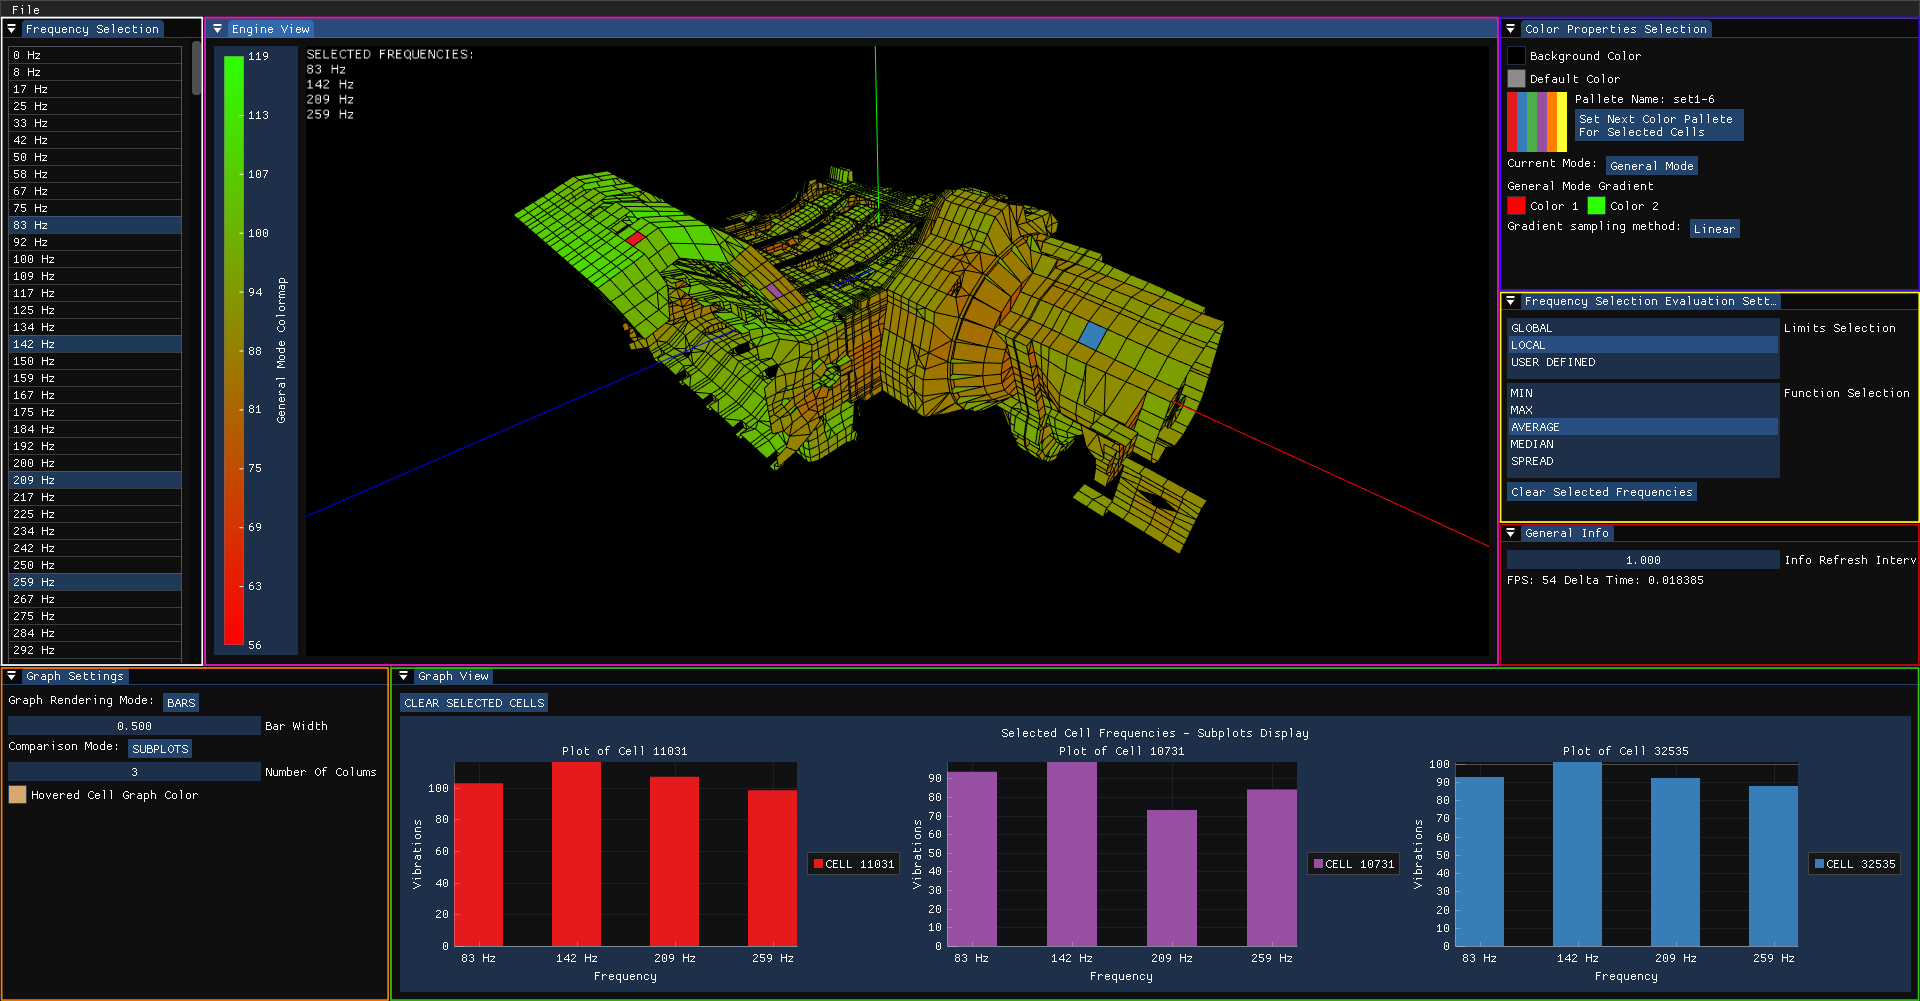
\includegraphics[width=\linewidth]{general_screenshot_segmented.png}
\caption{Prozori koji čine alat: prikaz motora (ružičasta) i grafa (zelena), postavke boja (plava), grafa (narančasta) i evaluacije frekvencija (žuta), odabir frekvencija (bijela) te općenite informacije (crvena)}
\label{fig:gen-screen}
\end{figure}

\section{Vrste analize motora} \label{work-mode-section}

Određivanje boje elementa modela motora s obzirom na niz frekvencija koje je korisnik odabrao predstavlja glavni izazov kod dizajniranja vizualizacijskog alata ove vrste. U sklopu ovog alata su implementirana dvije vrste analize koje se međusobno ne razlikuju samo u izvedbi, već i u primjeni zbog čega se dobro upotpunjuju.

\subsection{Općenita analiza vibracija} \label{normal-mode-section}

Općenita analiza iscrtavanja je odgovor alata na zahtjev \ref{req:general-vis}, a funkcionira tako da korisnik odabere niz frekvencija vibriranja, zatim se za svaki element izdvoji niz podataka o snagama vibracija tog elementa koji se preda kao argument funkciji koja ga "sažme" u jedan broj. U sklopu alata je implementirano nekoliko funkcija koje obavljaju tu zadaću, a korisnik odabire onu koja mu najviše odgovara. Implementirane funkcije su:

\begin{itemize}
\item MIN - najmanji iznos vibracije,
\item MAX - najveći iznos,
\item AVERAGE - prosjek vibracija,
\item MEDIAN - medijan vibracije,
\item SPREAD - razlika između najvećeg i najmanjeg iznosa vibracije.\\
\end{itemize}

Glavna ideja općenite analize vibracija je da se vrijednost dobivena iz navedenih funkcija koristi za uzorkovanje gradijenta kojeg korisnik definira. No, prije nego se ta vrijednost može koristiti za uzorkovanje, potrebno ju je prebaciti u interval [0, 1]. Za ostvarivanje prijelaza u taj interval je potrebno definirati broj koji označava najmanju vrijednost intervala, odnosno 0, kao i broj koji označava najveću vrijednost intervala, odnosno 1. U alatu su ponuđena tri načina računanja navedenog raspona:

\begin{itemize}
\item GLOBAL - donju i gornju granicu raspona čine najmanji i najveći iznos snage vibracije kojom neki element može vibrirati s obzirom na odabrane frekvencije vibriranja,
\item LOCAL - donju i gornju granicu raspona čine najmanji i najveći iznos snage vibracije kojom neki element može vibrirati s obzirom na odabrane frekvencije vibriranja,
\item USER DEFINED - korisnik sam definira donju i gornju granicu raspona.\\
\end{itemize}

\subsection{Analiza vibracija s preddefiniranim ograničenjima} \label{limits-mode-section}

Druga vrsta analize koja je implementirana u ovom alatu je bazirana na unaprijed određenim ograničenjima vibracija, te pruža odgovor na zahtjev \ref{req:limited-vis}. Navedena ograničenja (objašnjena u poglavlju \ref{area-overview-section}) su definirana za određene frekvencije (ne nužno za sve), a nalaze se u posebnoj datoteci koju korisnik učitava u alat. U ovoj vrsti analize, elementi se raspoređuju u navedene zone s obzirom na frekvencije vibriranja koje korisnik odabere, po sljedećim pravilima:

\begin{itemize}
\item Bezopasna zona - element vibrira snagom koja je u granicama bezopasne zone s obzirom na sve odabrane frekvencije,
\item Rizična zona - element vibrira snagom koja je u granicama rizične zone s obzirom na barem jednu odabranu frekvenciju, a za nijednu odabranu frekvenciju se ne nalazi u opasnoj zoni,
\item Opasna zona - element vibrira snagom koja je u granicama opasne zone s obzirom na barem jednu odabranu frekvenciju.\\
\end{itemize}

Boja elementa koji se nalaze u bezopasnoj zoni je konstantna za sve elemente u toj zoni. S druge strane, boje elemenata koji se nalaze u ostale dvije zone se određuju uzorkovanjem dva različita gradijenta. Navedeni gradijenti se uzorkuju pomoću omjera broja frekvencija vibriranja tijekom kojih snaga vibracije elementa spada u zonu gradijenta i ukupnog broj odabranih frekvencija. Iako navedena boja i gradijenti imaju početno zadane vrijednosti, korisnik ih može mijenjati kako njemu odgovara.\\


\section{Prikaz motora} \label{engine-view-section}
Zadaća prikaza motora je jasno vizualizirati podatke o vibracijama elemenata, pritom uzimajući u obzir brojne postavke vizualizacije poput: vrste analize, odabranih frekvencija, načina računanja konačnih podataka elemenata, zadanih raspona podataka te gradijenata koje se koristi za vizualizaciju. Korisnik ovu komponentu također koristi za označavanje interesnih elemenata.

\begin{figure}[H]
\centering
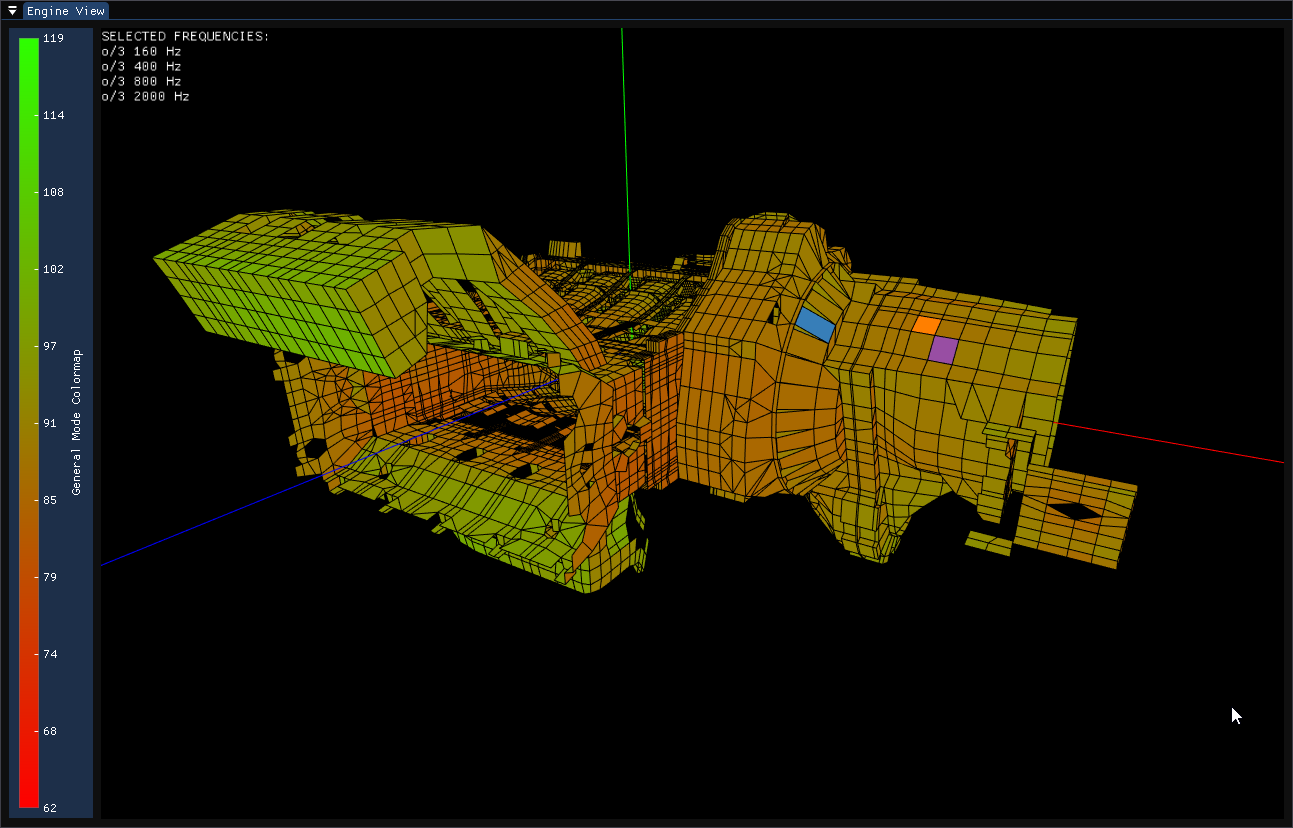
\includegraphics[width=0.85\linewidth]{engine_view_normal_mode.png}
\caption{Prikaz motora tijekom općenite analize vibracije}
\label{fig:normal-mode-engine-view}
\end{figure}
\begin{figure}[h]
\centering
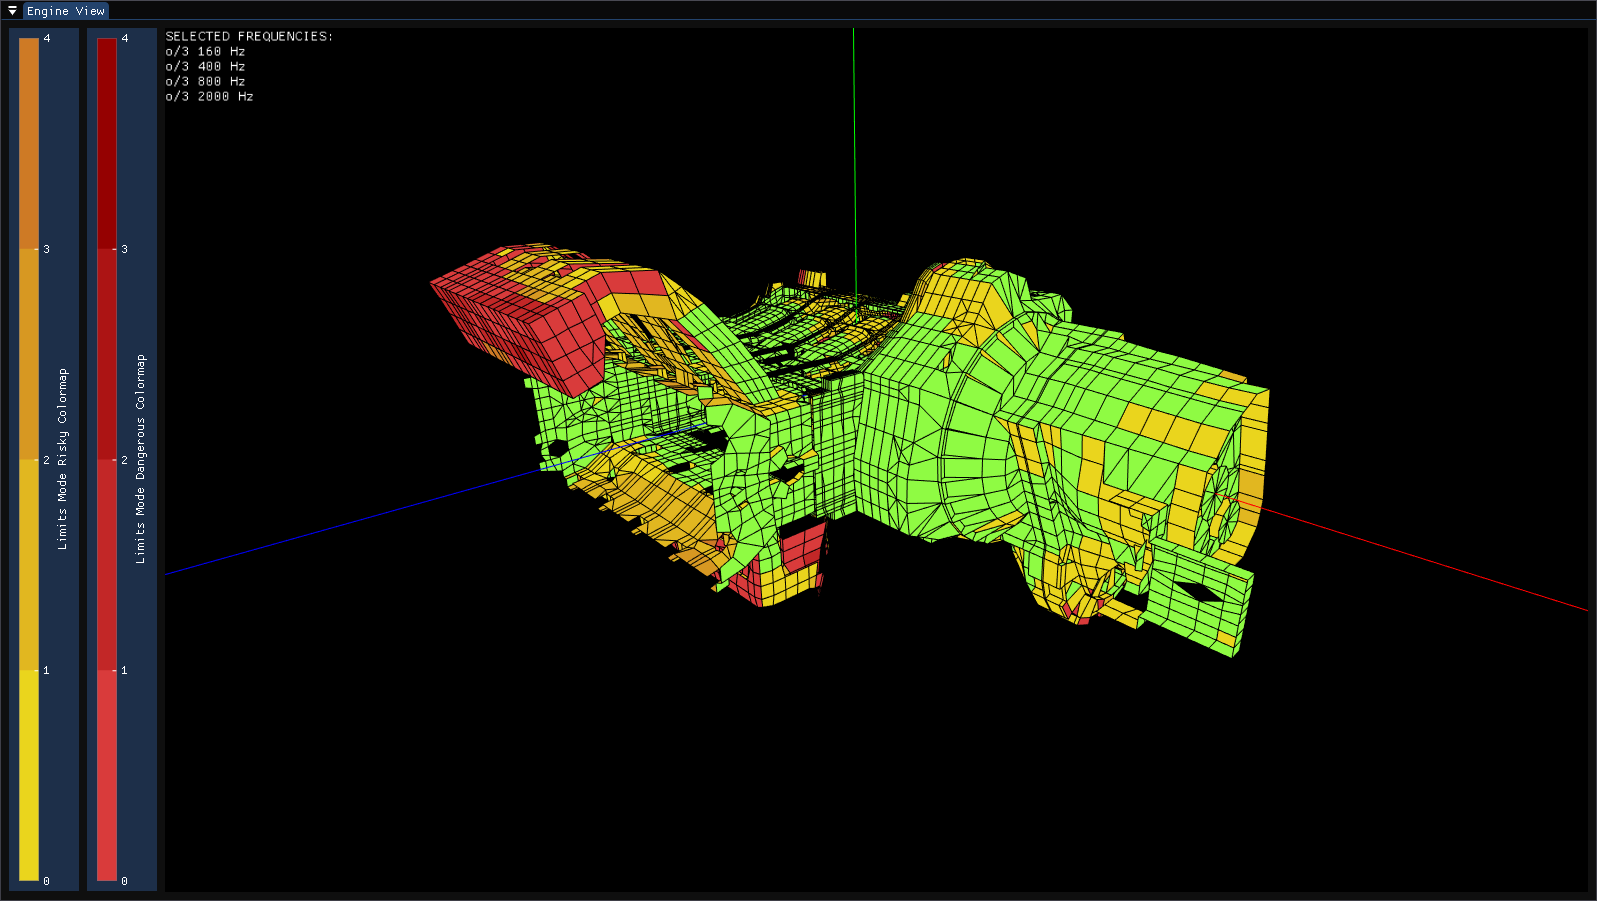
\includegraphics[width=0.85\linewidth]{engine_view_limits.png}
\caption{Prikaz motora tijekom analize s preddefiniranim ograničenjima}
\label{fig:limits-mode-engine-view}
\end{figure}

Na slikama \ref{fig:normal-mode-engine-view} i \ref{fig:limits-mode-engine-view} se može vidjeti primjer ovog prikaza tijekom dvije moguće analize vibracije. Uz prikaz obojanog modela ova komponenta alata je zadužena i za prikaz legende gradijenta i nabrajanje odabranih frekvencija vibriranja, kako bi snimak prikaza prenosio sve relevantne informacije potrebne za razumijevanje rezultata vizualizacije. Osi koordinatnog sustava su nacrtane uz model motora kako bi korisnik dobio osjećaj za 3D prostor u kojem se model nalazi. Omogućeno je označavanje elementa kako bi se zadovoljio zahtjev \ref{req:multi-cell}, a vrši se pozicioniranjem pokazivača miša iznad interesnog elementa te klikom na lijevu tipku miša. Kada korisnik pokazivačem miša prijeđe preko elementa bez klikanja, boja elementa postaje inverz prijašnje boje, kako bi se korisniku dala povratna informacija o elementu koji će biti odabran odluči li se korisnik kliknuti lijevu tipku miša. Opisani element će se u nastavku rada nazivati "lebdeći" element. Jednom kada korisnik klikne na element, odabrani element se označava jednom od boja iz trenutne palete (detaljno objašnjeno u poglavlju \ref{color-settings-section}) čime se zadovoljava zahtjev \ref{req:selected-cell-emp}, te se korisniku prikazuje detaljan uvid u podatke označenog elementa putem prikaza grafa (vidi poglavlje \ref{graph-view-section}). Ponovnim klikom na već odabrani element, on se briše iz liste odabranih elemenata.\\

Kao što je vidljivo iz slika \ref{fig:normal-mode-engine-view} i \ref{fig:limits-mode-engine-view}, razlike između dvije vrste analize se ne manifestiraju samo u vizualizaciji motora, već i u sučelju ovog prikaza. Naime, kako je objašnjeno u poglavlju \ref{normal-mode-section}, u općenitoj analizi vibracija je alatu potreban jedan kontinuirani gradijent, a u analizi s preddefiniranim ograničenjima su potrebna dva diskretna gradijenta.

\begin{figure} [H]
     \centering
     \begin{subfigure}[h]{0.17\textwidth}
         \centering
         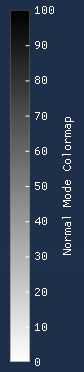
\includegraphics[width=\textwidth]{linear_colormap.png}
         \caption{Linearno}
         \label{fig:linear_legend}
     \end{subfigure}
     \hfill
     \begin{subfigure}[h]{0.17\textwidth}
         \centering
         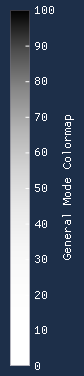
\includegraphics[width=\textwidth]{cubic_colormap.png}
         \caption{Kubno v1}
         \label{fig:cubic_legend}
     \end{subfigure}
     \hfill
     \begin{subfigure}[h]{0.17\textwidth}
         \centering
         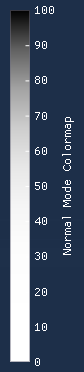
\includegraphics[width=\textwidth]{quartic_colormap.png}
         \caption{Kvartičko v1}
         \label{fig:quartic_legend}
     \end{subfigure}
     \hfill
     \begin{subfigure}[h]{0.17\textwidth}
         \centering
         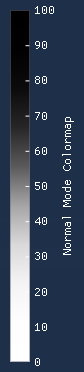
\includegraphics[width=\textwidth]{cubic_symmetrical_colormap.png}
         \caption{Kubno v2}
         \label{fig:cubic_symmetrical_legend}
     \end{subfigure}
     \hfill
     \begin{subfigure}[h]{0.17\textwidth}
         \centering
         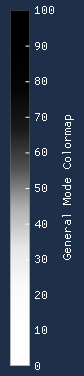
\includegraphics[width=\textwidth]{quartic_symmetrical_colormap.png}
         \caption{Kvartičko v2}
         \label{fig:quartic_symmetrical_legend}
     \end{subfigure}
        \caption{Drugačije postavke uzorkovanja gradijenta}
        \label{fig:colormap-legends}
\end{figure}

Osim što je navedene gradijente moguće mijenjati pomoću dvije kontrolne boje, moguće ih je mijenjati i promjenom funkcije uzorkovanja gradijenta. Navedeni dodatak je uveden kako bi vizualizacija bila indiferentna na distribuciju podataka na zadanom rasponu, te kako bi se omogućilo isticanje elemenata koji se nalaze na "rubovima" gradijenta, čime se zadovoljava zahtjev \ref{req:cell-emphasis}. Utjecaj različitih funkcija uzorkovanja na kontinuirane gradijente se može vidjeti na slici \ref{fig:colormap-legends}. Različite funkcije uzorkovanja su izravno preuzete s web stranice Easing \citep{easing}.

\section{Prikaz grafa} \label{graph-view-section}

Komponenta prikaza grafa služi za iscrtavanje jednog ili više prikaza grafova odabranih elemenata, ali i "lebdećeg" elementa. Ova komponenta je odgovor na zahtjev \ref{req:multi-cell}, ali kako je već spomenuto, za određene zahtjeve često nije moguće pronaći jednu vizualizacijsku tehniku koja savršeno rješava problem, već je nužno implementirati niz tehnika koje se upotpunjuju. Stoga su u sklopu alata implementirana dva načina iscrtavanja podataka: stupčasti i linijski, te tri načina uspoređivanja:
\begin{itemize}
\item Općeniti način usporedbe (DEFAULT) - svi grafovi su prikazani unutar jednog prikaza,
\item Način usporedbe s višestrukim prikazima (SUBPLOTS) - svaki graf je prikazan unutar zasebnog prikaza,
\item Relativni način usporedbe (RELATIVE) - kao općeniti način, ali je dodana mogućnost odabiranja elementa s obzirom na koji će se prikazati grafovi svih ostalih elemenata.\\
\end{itemize}

Navedeno rješenje predstavlja poboljšanje na području čitljivosti u odnosu na alat razvijen u radu Matkovića et al. \citep{matkovic2021getting} zbog više razloga. Više nisu odjednom prikazani grafovi svih elemenata, već samo odabranih. Moguće je prikazati svaki graf na zasebnom prikazu, čime je pojednostavljeno uspoređivanje u slučaju više odabranih elemenata. S relativnim uspoređivanjem, korisnik može lakše usporediti odabrani element s ostalim elementima. Konačno, budući da su omogućena dva načina iscrtavanja podataka, korisnik može odabrati način koji najbolje odgovara njegovim potrebama i preferencijama. Boje grafova odabranih elemenata odgovaraju bojama koje ti elementi imaju unutar prikaza motora (vidi poglavlje \ref{engine-view-section}), čime se dodatno zadovoljava zahtjev \ref{req:selected-cell-emp}, a boja grafa "lebdećeg" elementa je zadana unutar postavki grafa (vidi poglavlje \ref{graph-settings-section}). Na slici \ref{fig:default_graph_display_bars} je vidljivo kako ovu komponentu čini jedan ili više prikaza grafova i gumb za brisanje liste odabranih elemenata.

\begin{figure}[H]
	\centering
	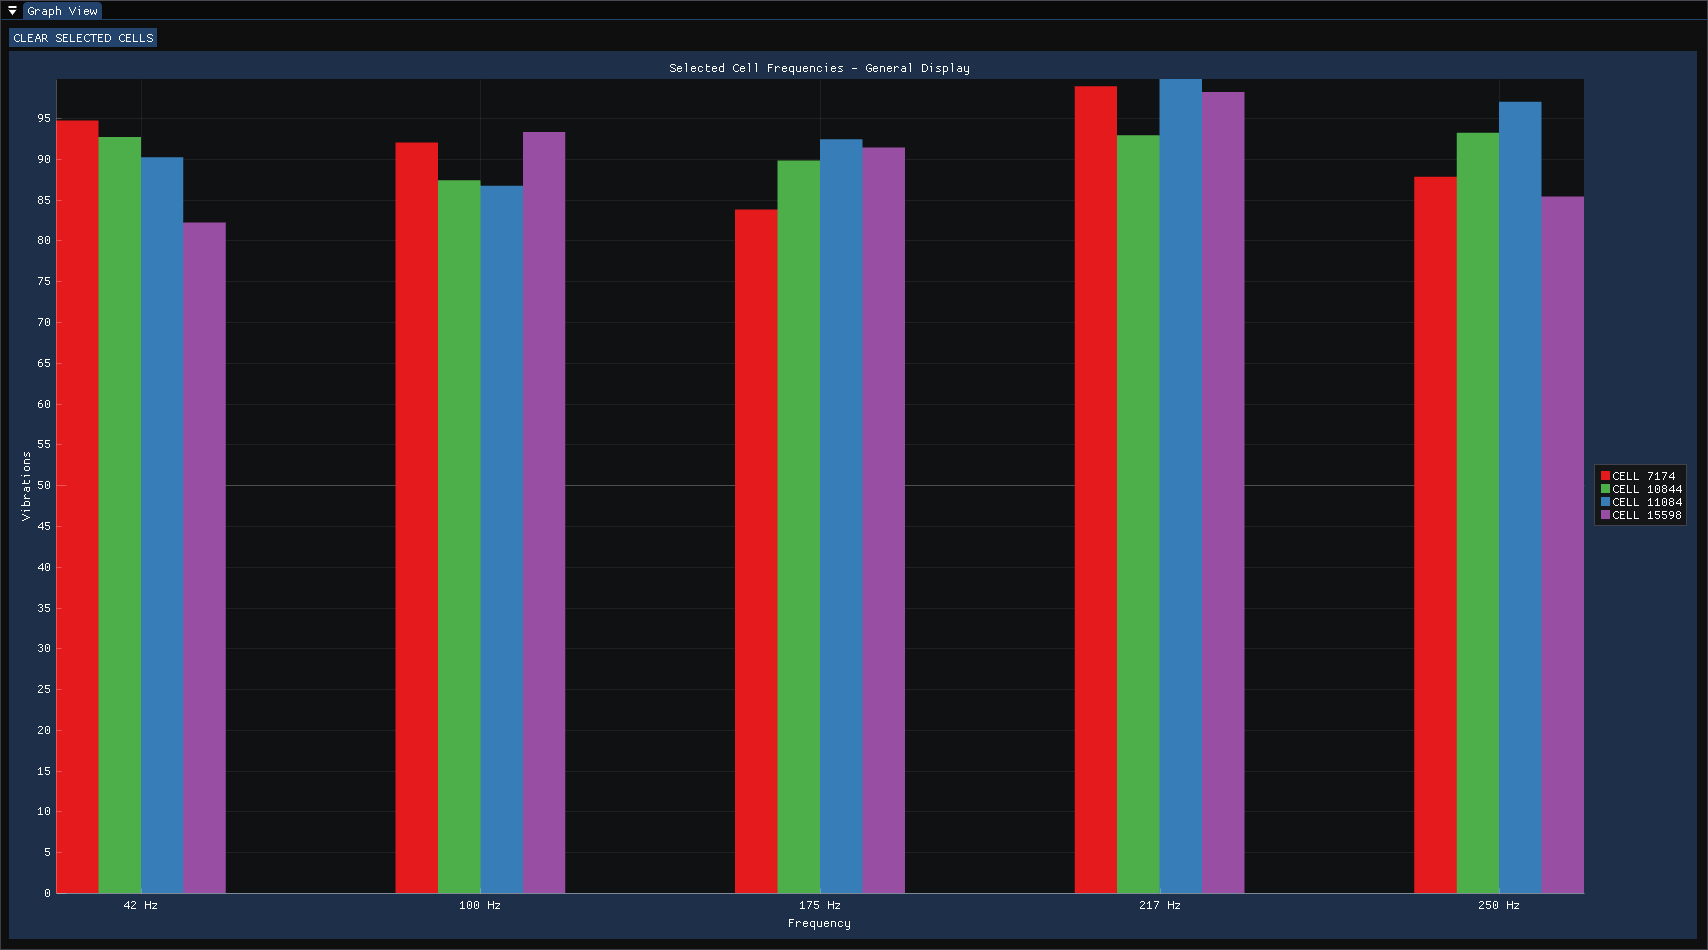
\includegraphics[width=0.9\textwidth]{default_graph_display_bars.png}
	\caption{Općeniti način usporedbe grafova u obliku stupaca}
    \label{fig:default_graph_display_bars}
\end{figure}

Iz priloženih slika je također vidljivo kako su rasponi osi prikaza grafova postavljeni tako da obuhvaćaju podatke koji se u njima nalaze, te nisu fiksno određeni. Implementacija ovakvog načina određivanja raspona je odabrana zbog smanjene preglednosti razlika u "tokovima" grafova kod fisknih raspona jer pri fiksno zadanim rasponima grafovi često zauzimaju mali dio prikaza, a ostatak prikaza je potrošen na prazan prostor. Spomenuta primjedba je posebno uočljiva na slikama \ref{fig:subplots_graph_display_bars} i \ref{fig:subplots_graph_display_lines} gdje se vidi kako grafovi koji su iscrtani pomoću stupaca bolje prikazuju razliku u iznosima podataka, ali grafovi iscrtani pomoću linija bolje prikazuju razlike u "tokovima" grafova. Konkretno, na slici \ref{fig:subplots_graph_display_bars} se na prvi pogled čini kako se svi elementi ponašaju slično, no uvidom u graf na slici \ref{fig:subplots_graph_display_lines} se otkriva kako to nije istina.

\begin{figure}[H]
	\centering
	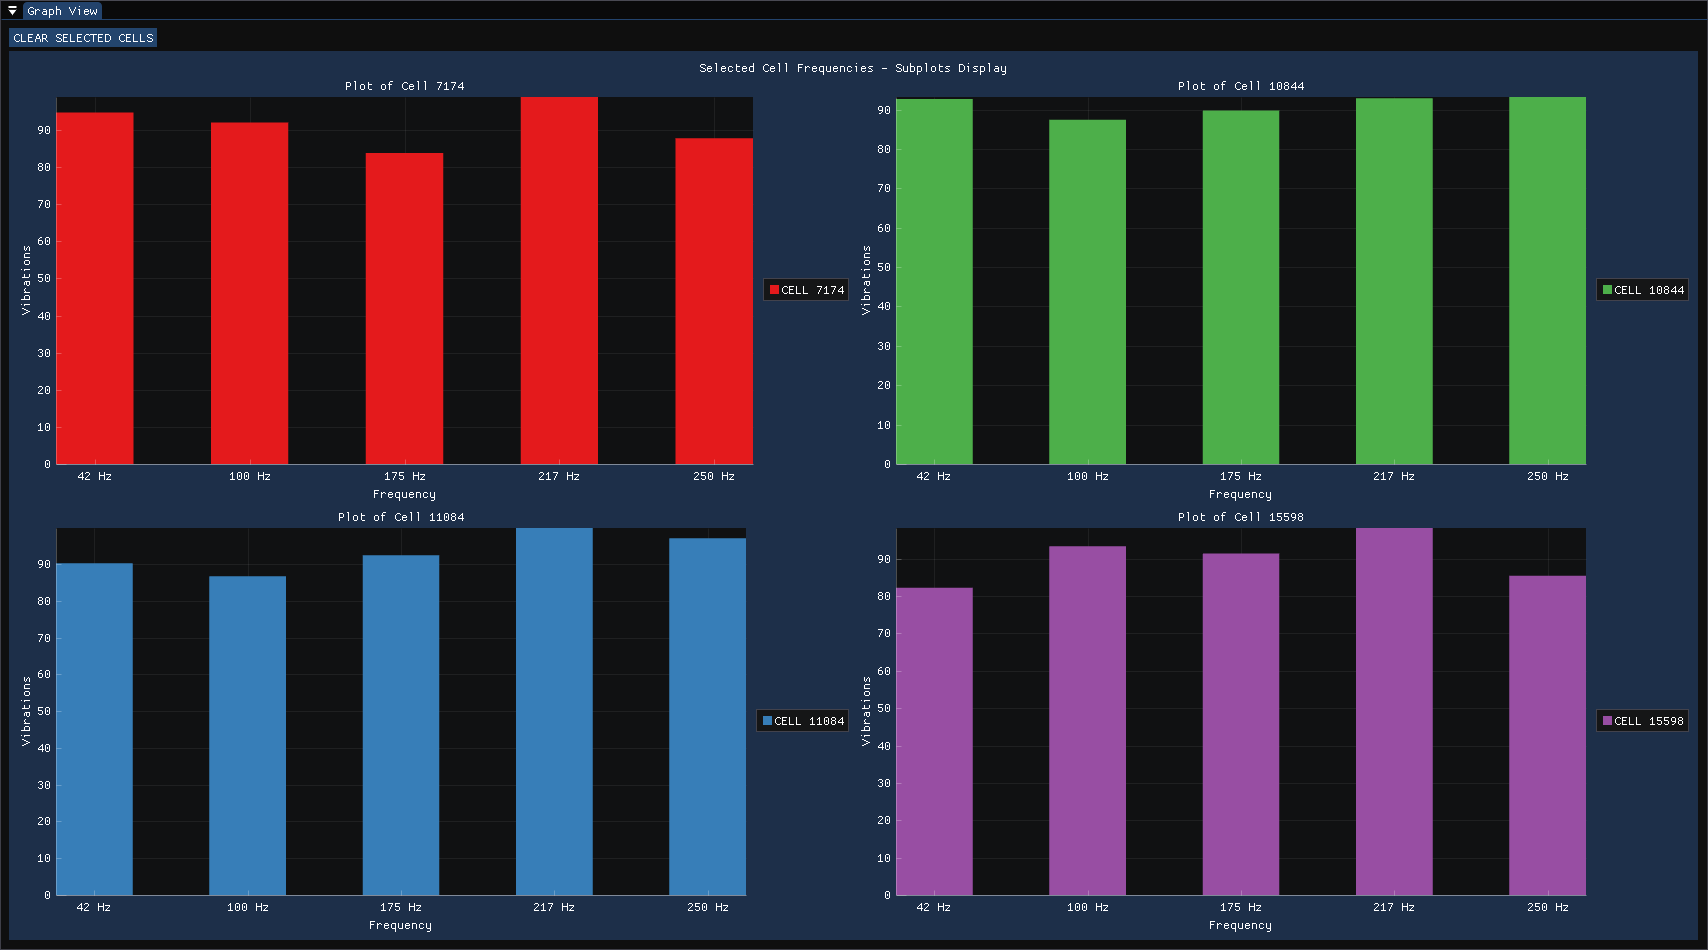
\includegraphics[width=0.9\textwidth]{subplots_graph_display_bars.png}
	\caption{Način usporedbe grafova s višestrukim prikazima u obliku stupaca}
    \label{fig:subplots_graph_display_bars}
\end{figure}

\begin{figure}[H]
	\centering
	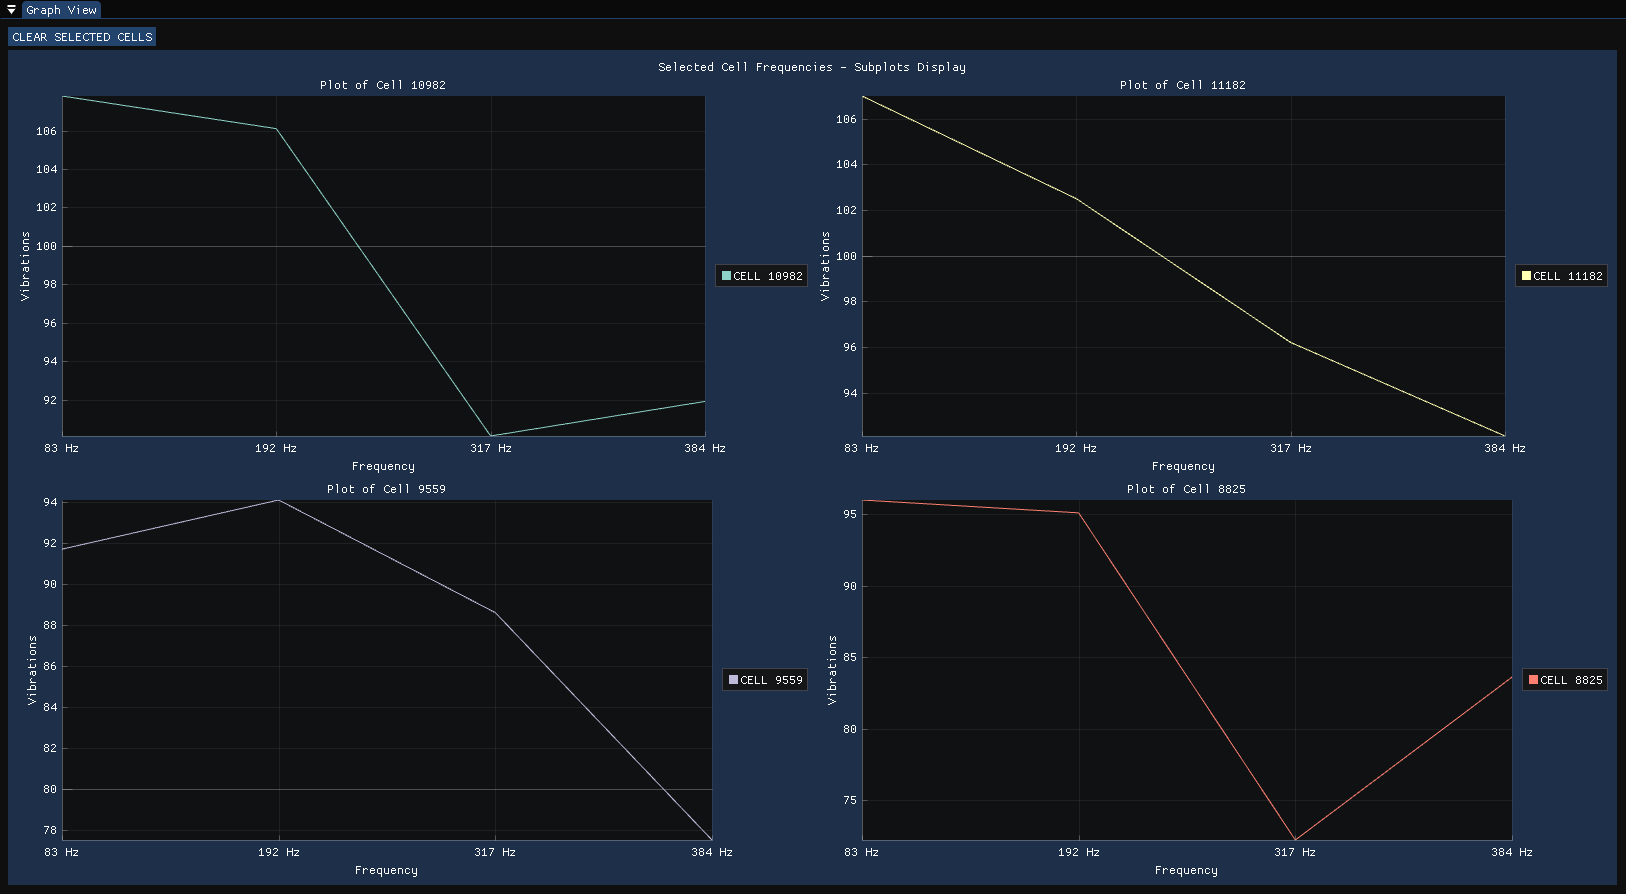
\includegraphics[width=0.9\textwidth]{subplots_graph_display_lines.png}
	\caption{Način usporedbe grafova s višestrukim prikazima u obliku linija}
    \label{fig:subplots_graph_display_lines}
\end{figure}

Korisnik dodatno može namjestiti odgovarajući raspon pojedinih osi pomoću postavki osi koje je moguće otvoriti klikom na desnu tipku miša dok je pokazivač miša postavljen iznad željene osi. Kao što se vidi na slici \ref{fig:graph-axis-settings}, unutar spomenutih postavki je moguće uređivati brojna svojstva osi poput raspona, načina interpoliranja između granica raspona, smjera osi itd.

\begin{figure} [H]
	\centering
    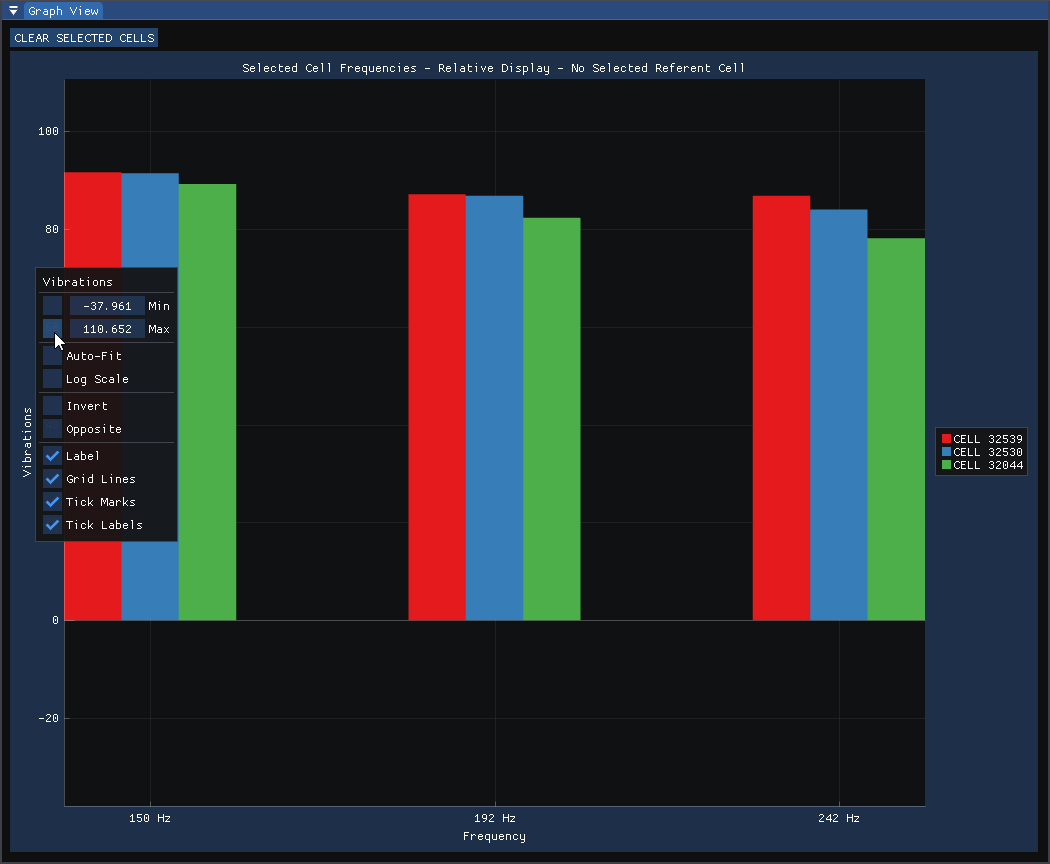
\includegraphics[width=0.9\textwidth]{graph_view_axis_settings.png}
    \caption{Postavke osi prikaza grafa}
    \label{fig:graph-axis-settings}
\end{figure}

\section{Postavke boja} \label{color-settings-section}
Kao što samo ime ove komponente kaže, glavna svrha joj je čuvanje postavki koje bi mijenjale boje i gradijente unutar prikaza motora. Na slici \ref{fig:color-settings-2-modes} mogu se vidjeti razlike u komponenti između dvije vrste analize. U obje vrste analize je moguće promijeniti pozadinsku boju prikaza motora, boju koju motor ima kad nijedna frekvencija nije odabrana, paletu za odabrane elemente i trenutnu vrstu analize. No, dva prikaza postavki boja se ipak djelomično razlikuju jer je za općenitu analizu vibracija potrebno definirati samo jedan gradijent, a za analizu s preddefiniranim ograničenjima je potrebno definirati jednu boju (za sigurnu zonu) i dva gradijenta (za rizičnu i opasnu zonu).

\begin{figure} [H]
     \centering
     \begin{subfigure}[h]{0.49\textwidth}
         \centering
         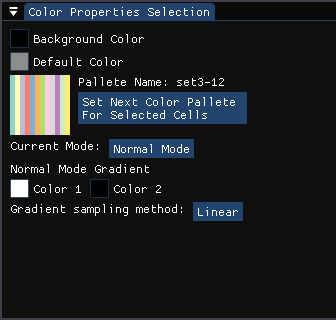
\includegraphics[width=\textwidth]{color_settings_normal_mode.png}
         \caption{Općenita analiza vibracija}
         \label{fig:color-settings-normal-mode}
     \end{subfigure}
     \hfill
     \begin{subfigure}[h]{0.49\textwidth}
         \centering
         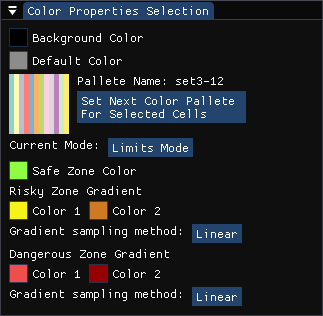
\includegraphics[width=\textwidth]{color_settings_limits_mode.png}
         \caption{Analiza s preddefiniranim ograničenjima}
         \label{fig:color-settings-limits-mode}
     \end{subfigure}
     \caption{Postavke boja tijekom dva moguća načina rada}
     \label{fig:color-settings-2-modes}
\end{figure}

Što se tiče mijenjanja postavki, korisnik može mijenjati boje klikom na obojani kvadrat čime se otvara prozor za mijenjanje boja prikazan na slici \ref{fig:color-picker}. U otvorenom prozoru boju se može mijenjati pomoću interaktivnog GUI sučelja ili unosom RGB ili HSV vrijednosti boje, a također je moguće i unošenje boja u heksadekadskom formatu.

\begin{figure} [H]
	\centering
    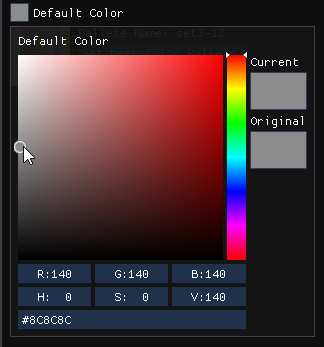
\includegraphics[width=0.5\textwidth]{color_settings_color_picker.png}
    \caption{Prozor za odabir boje}
    \label{fig:color-picker}
\end{figure}

Palete boja za odabrane elemente su učitane izravno iz datoteke \textit{default\_pallete.txt} koja se mora nalaziti u istom direktoriju kao i izvršna datoteka alata. Početne palete su preuzete s web stranice ColorBrewer \citep{colorbrewer} kako bi se postiglo što bolje isticanje odabranih elemenata, te su unesene u navedenu datoteku u sljedećem formatu:

\begin{lstlisting}
p ime_palete
rgb_vrijednosti_boje1_u_rasponu_0_255
rgb_vrijednosti_boje2_u_rasponu_0_255
rgb_vrijednosti_boje3_u_rasponu_0_255
rgb_vrijednosti_boje4_u_rasponu_0_255
\end{lstlisting}
\ 
\\

Na slici \ref{fig:color-settings-2-modes} se može vidjeti kako je za svaku paletu u kvadratiću prikazan spektar boja, desno od kojeg je navedeno ime palete, a ispod imena se nalazi gumb za prelazak na sljedeću paletu. Kako palete sadrže ograničen broj boja, u alatu je implementirano brisanje odabranih elemenata kada je njihov broj veći od broja boja u paleti. Postoje dva takva slučaja: dodavanje novog elementa kada su već sve boje palete "zauzete" i mijenjanje trenutne palete na paletu čiji je broj boja manji od broja trenutno odabranih elemenata. U prvom slučaju alat briše zadnji odabrani element i dodaje novoodabrani element, a u drugom slučaju alat briše onoliko zadnjih odabranih elemenata kolika je razlika između broja odabranih elemenata i broja boja nove palete.\\

Ispod sučelja za mijenjanje palete se nalazi gumb za mijenjanje načina rada. Na gumbu piše ime trenutne vrste analize, a klikom na gumb alat prelazi u sljedeću vrstu analize. Kako su moguće samo dvije vrste analize, gumb će alternirati između općenite analize i analize s preddefiniranim ograničenjima.\\

Konačno, sučelje za odabir gradijenta se sastoji od dva standardna kvadrata za mijenjanje boja pomoću kojih se mijenja početna i krajnja kontrolna boja gradijenta. Ispod navedenih kvadrata se nalazi gumb za mijenjanje metode uzorkovanja gradijenta. Implementirane metode uzorkovanja i njihov utjecaj na gradijent su objašnjene i prikazane u poglavlju \ref{graph-view-section}.

\section{Postavke grafa} \label{graph-settings-section}

Postavke grafa se dijele na tri dijela koji su jasno naznačeni na slici \ref{fig:graph-settings-segmented}. Dio u kojem se mijenja boja grafa lebdećeg elementa se ne mijenja s obzirom na različite načine crtanja ili uspoređivanja jer se taj graf uvijek iscrtava. Kao što je već napomenuto u poglavlju \ref{graph-view-section}, alat implementira dva načina iscrtavanja grafa: linijski i stupčasti, a razlika u postavkama između ta dva načina je što stupčastom grafu korisnik može odrediti širinu stupca, kao što se može vidjeti na slici \ref{fig:graph-settings-segmented}, dok na linijskom grafu korisnik ne može mijenjati ništa. Način iscrtavanja se mijenja klikom na gumb na kojem piše ime trenutno aktivnog načina iscrtavanja.

\begin{figure} [H]
	\centering
    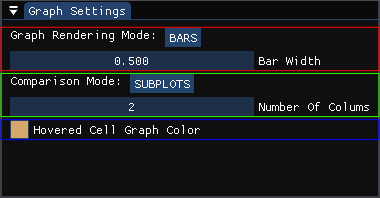
\includegraphics[width=0.7\textwidth]{graph_settings_subplots_segmented.png}
    \caption{Postavke grafa rastavljene na dijelove: postavke načina iscrtavanja (crveno), postavke načina usporedbe (zeleno) i postavke boje grafa "lebdećeg" elementa (plavo)}
    \label{fig:graph-settings-segmented}
\end{figure}

Ali za razliku od postavki načina iscrtavanja, razlike između postavki načina uspoređivanja su puno uočljivije. Tijekom općenitog načina usporedbe, korisnik nema nikakvih dodatnih postavki osim gumba za mijenjanje načina usporedbe koji je prisutan tijekom svih načina uspoređivanja i funkcionira na identičan način kao i gumb za mijenjanje načina iscrtavanja. Tijekom načina usporedbe s višestrukim prikazima, korisnik može odabrati u koliko će se stupaca prikazi organizirati. Konačno, kada je aktivan relativni način usporedbe, korisnik može odabrati jednog od već odabranih elemenata s obzirom na kojeg će se prikazati grafovi ostalih elemenata. Gumb elementa kojeg korisnik odabere, ali i gumb elementa iznad kojeg korisnik postavi pokazivač miša poprima boju odgovarajućeg elementa iz prikaza motora. Navedeni dodatak je implementiran kako bi korisnik imao bolju ideju o tome koji element je trenutno odabran i/ili koji će element biti odabran za relativno iscrtavanje.

\begin{figure} [H]
     \centering
     \begin{subfigure}[h]{0.495\textwidth}
         \centering
         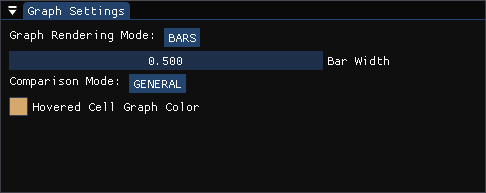
\includegraphics[width=\textwidth]{graph_settings_default.png}
         \caption{Općeniti način usporedbe}
         \label{fig:graph-settings-normal-mode}
     \end{subfigure}
     \hfill
     \begin{subfigure}[h]{0.495\textwidth}
         \centering
         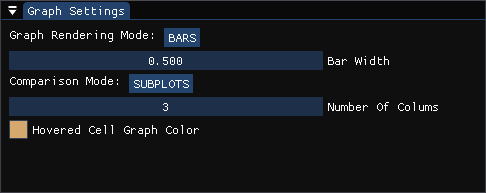
\includegraphics[width=\textwidth]{graph_settings_subplots.png}
         \caption{Način usporedbe s višestrukim prikazima}
         \label{fig:graph-settings-limits-mode}
     \end{subfigure}
     \hfill
     \begin{subfigure}[h]{0.495\textwidth}
         \centering
         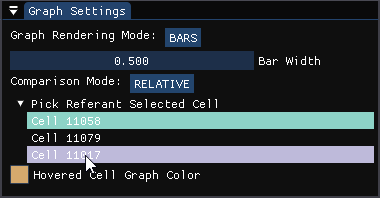
\includegraphics[width=\textwidth]{graph_settings_relative.png}
         \caption{Relativni način usporedbe}
         \label{fig:graph-settings-limits-mode}
     \end{subfigure}
     \caption{Postavke grafa tijekom tri različita načina usporedbe}
     \label{fig:graph-settings-3-modes}
\end{figure}

\section{Odabir frekvencija} \label{frequency-selection-section}

Ova komponenta služi isključivo za odabir frekvencija (kao što i samo ime govori), a odvojena je od postavki evaluacije odabranih frekvencija (opisanih u poglavlju \ref{frequency-settings-section}) zbog olakšavanja korištenja alata. Izgled komponente se može vidjeti na slici \ref{fig:frequency-selection-view}. U općenitoj analizi, vibracija komponenta prikazuje sve frekvencije za koje su učitani podaci o vibriranju elemenata, dok su u analizi vibracija s preddefiniranim ograničenjima prikazane samo frekvencije za koje su definirana ograničenja u datoteci s ograničenjima. Pomoću ove komponente korisnik može odabrati proizvoljan broj frekvencija, čime se zadovoljava zahtjev \ref{req:multi-freq}.

\begin{figure} [H]
	\centering
    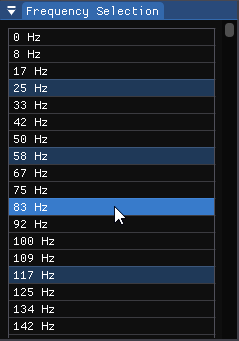
\includegraphics[width=0.8\textwidth]{frequency_selection_view.png}
    \caption{Prozor za odabir frekvencija}
    \label{fig:frequency-selection-view}
\end{figure}

\section{Postavke evaluacije odabranih frekvencija} \label{frequency-settings-section}

Kao što je već opisano u poglavlju \ref{normal-mode-section}, korisnik u općenitoj analizi vibracija može dodatno prilagoditi prikaz snaga vibracije dijelova motora odabirom različitih metoda pomoću kojih se iz niza podataka o snazi vibracija elementa dobije jedan konkretan podatak. Zatim se pomoću odabranog raspona izračunati podatak pretvara u podatak iz raspona [0, 1] kako bi se olakšalo uzorkovanje gradijenta. Navedene prilagodbe nisu moguće prilikom analize s preddefiniranim ograničenjima jer je algoritam već "strogo" zadan i nema dijelova algoritma koje korisnik može mijenjati, ali spomenute parametre općenite analize vibracija, korisnik može mijenjati unutar komponente postavki odabranih frekvencija koja je prikazana na slici \ref{fig:frq-sel-eval-settings}.

\begin{figure} [H]
	\centering
    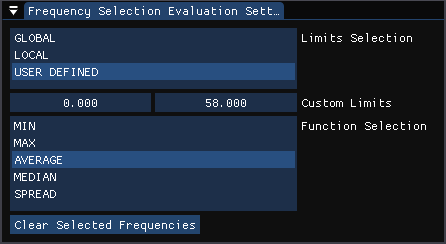
\includegraphics[width=0.8\textwidth]{frq_sel_eval_settings.png}
    \caption{Prozor postavki evaluacije odabranih frekvencija sa svim mogućim parametrima}
    \label{fig:frq-sel-eval-settings}
\end{figure}

Prozor postavki evaluacije odabranih frekvencija nije vidljiv sve dok korisnik ne odabere jednu od ponuđenih frekvencija unutar komponente iz poglavlja \ref{frequency-selection-section}. Kada se odabere barem jedna frekvencija, prozor postavki se prikazuje s parametrima koji su vidljivi ovisno o broju odabranih frekvencija i vrsti analize koju korisnik upotrebljava.\\

Obje vrste analize u postavkama imaju gumb za brisanje liste trenutno odabranih frekvencija. Analiza vibracija s preddefiniranim ograničenjima osim tog gumba u postavkama nema niti jedan drugi element, dok u općenitoj analizi korisnik u postavkama može mijenjati već spomenute metode računanja konačnih podataka i raspone izračunatih podataka. Lista za odabir raspona je vidljiva kada korisnik odabere barem jednu frekvenciju, a mijenjanje raspona definiranog od korisnika je omogućeno kada je navedeni raspon odabran u spomenutoj listi. Lista za odabir metoda računanja konkretnih podataka je vidljiva kada korisnik odabere dvije ili više frekvencije jer se pri jednoj odabranoj frekvenciji sve funkcije ponašaju identično.


\section{Općenite informacije} \label{general-info-section}

Na slici \ref{fig:general-info} se može vidjeti komponenta koja služi za prikaz općenitih informacija vezanih za performanse alata poput broja sličica po sekundi i vremena proteklog između iscrtavanja dviju sličica. Korisnik dodatno može promijeniti interval nakon kojeg se navedene informacije ažuriraju.

\begin{figure} [H]
	\centering
    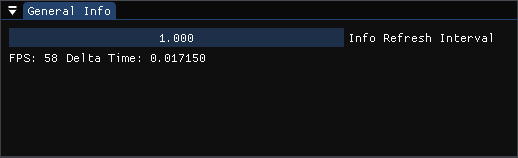
\includegraphics[width=0.9\textwidth]{general_info.png}
    \caption{Prozor za općenite informacije}
    \label{fig:general-info}
\end{figure}

\chapter{Implementacija}

Alat je razvijen u programskom jeziku C++ uz korištenje biblioteke OpenGL za komuniciranje s grafičkom karticom. No, osim OpenGL-a, za razvoj alata je korišten i niz drugih biblioteka, čiji su detaljniji opisi i razlozi za korištenje navedeni u poglavlju \ref{libraries-section}. Budući da su se tijekom razvoja alata konstantno pojavljivali novi zahtjevi i funkcionalnosti koje je trebalo implementirati, bilo je potrebno uspostaviti arhitekturu koje će se rješenje pridržavati kako ne bi postalo kruto i krhko, a ta arhitektura je opisana u poglavlju \ref{codebase-architecture-section}. Konačno, kako je način slanja podataka s procesora na grafičku karticu iznimno važna komponenta izvedbe svake grafičke aplikacije, poglavlje \ref{graphics-card-data-section} opisuje kako je organiziran tok podataka s procesora na grafičku karticu.

\section{Korištene biblioteke} \label{libraries-section}

\subsection{OpenGL}

OpenGL \citep{opengl} je višeplatformska i višejezična biblioteka koja služi za prikazivanje 2D i 3D vektorske grafike. Biblioteka podržava dva distinktna načina rada: \textit{compatibility} i \textit{core}. U \textit{compatibility} načinu rada klijent definira poziciju i boju točaka primitiva koje želi iscrtati pozivajući funkcije API-a, nakon čega se navedene točke propuštaju kroz fiksni grafički protočni sustav na kraju kojega se iscrtava slika. \textit{Core} način rada, često zvani moderni OpenGL, dopušta klijentu mijenjanje određenih dijelova grafičkog protočnog sustava pomoću sjenčara \engl{shader}. Sjenčari su programi napisani u GLSL-u \engl{OpenGL Shading Language} koji se izvode na grafičkoj kartici, te manipuliraju podacima poslanim od strane klijenta preko OpenGL API-a u obliku tzv. \textit{buffer object}-a kako bi se postigli različiti vizualni efekti.\\

Za razvoj alata opisanog u ovom radu je korišten OpenGL 3.3 u \textit{core} načinu rada. Iako je u sklopu implementacije alata ova biblioteka prvenstveno korištena za iscrtavanje 3D modela motora, implementacije biblioteka Dear ImGui (poglavlje \ref{imgui-section}) i ImPlot (poglavlje \ref{implot-section}) korištene u ovom radu također koriste OpenGL za iscrtavanje elemenata korisničkog sučelja i 2D grafova.

\subsection{Dear ImGui} \label{imgui-section}
Dear ImGui \citep{imgui} je C++ biblioteka koja služi za iscrtavanje grafičkog korisničkog sučelja ili GUI-a \engl{Graphical User Interface}.\\

GUI biblioteke se obično mogu razvrstati na zadržane \engl{retained} i izravne \engl{immediate} s obzirom na korištene obrasce ažuriranja prikaza. Zadržane biblioteke interno čuvaju podatke o primitivima korisničkog sučelja koje treba iscrtati, a klijent pozivima metoda biblioteke ne može izravno utjecati na iscrtavanje tih primitiva, već jedino može mijenjati apstraktni model korisničkog sučelja. Na ovakav način zadržane biblioteke mogu dodatno optimizirati kako i kada će se izvršiti iscrtavanje elemenata. S druge strane, izravne GUI biblioteke omogućuju klijentu izravno pozivanje metoda za iscrtavanje elemenata korisničkog sučelja. Zbog toga klijent treba pozivati funkcije za iscrtavanje primitiva u svakoj iteraciji petlje ažuriranja aplikacije.\\

Dear ImGui spada u kategoriju izravnih GUI biblioteka. Ova biblioteka omogućuje jednostavno i brzo iteriranje GUI aplikacija, te unatoč tome što joj nedostaju određene funkcionalnosti koje se mogu naći u drugim GUI bibliotekama, i dalje je iznimno popularna u području razvoja GUI aplikacija zbog jednostavnosti korištenja i nadogradnje.

\subsection{ImPlot} \label{implot-section}

Iako Dear ImGui službeno podržava crtanje grafova, funkcionalnosti grafova implementiranih u sklopu ove biblioteke su iznimno ograničene. Iz tog razloga, za implementaciju grafova u ovom radu je korištena biblioteka ImPlot \citep{implot}. Ova biblioteka je proširenje Dear ImGui-a koje omogućava prikaz raznovrsnih interaktivnih grafova jednostavnim pozivanjem metoda za iscrtavanje. 

\subsection{Ostale biblioteke}
Osim već spomenutih biblioteka, za razvoj ovog alata je korištena još nekolicina drugih biblioteka koje su navedene u ovom poglavlju.\\

GLFW \citep{glfw} je višeplatformska biblioteka za razvoj OpenGL aplikacija, a u sklopu ove aplikacije biblioteka je korištena za stvaranje prozora, konteksta, javljanje događaja i primanje ulaza od korisnika.\\

GLM \citep{glm} je matematička biblioteka za grafičke aplikacije pisane u OpenGL-u. GLM nudi brojne klase i funkcije koje su dizajnirane i implementirane s istim konvencijama imenovanja i funkcionalnostima kao odgovarajući tipovi podataka i funkcije u GLSL-u. GLM je u ovom alatu korišten za operacije nad vektorima, te računanje matrica transformacije i projekcije.\\

NFD \citep{nfd} \engl{Native File Dialog} je višeplatformska C biblioteka koja pruža mogućnost otvaranja izvornog dijaloga za datoteke, a u sklopu alata je korištena prilikom učitavanja različitih datoteka s podacima o motoru.

\section{Arhitektura rješenja} \label{codebase-architecture-section}

Organizacija k\^{o}da alata je generalno inspirirana obrascom Model-Pogled-Upravljač ili MVC \engl{Model-View-Controller} kako bi se omogućilo lakše održavanje programa. Na slici \ref{fig:high-level-overview} se može vidjeti pojednostavljeni prikaz MVC organizacije alata s većinom ključnih klasa alata.

\begin{figure} [H]
	\centering
    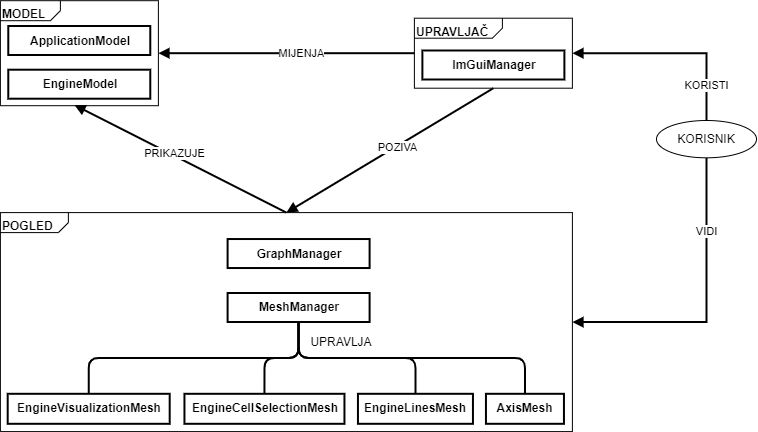
\includegraphics[width=\textwidth]{high_level_overview.png}
    \caption{Pregled MVC organizacije alata}
    \label{fig:high-level-overview}
\end{figure}

Važno je spomenuti kako na slici \ref{fig:high-level-overview} nedostaje glavna klasa alata, a to je klasa \textit{App} jer ne sudjeluje izravno u MVC arhitekturi. Glavna odgovornost ove klase je povezivanje prikazanih komponenti, obrađivanje GLFW događaja i pozivanje metoda za ažuriranje spomenutih komponenti tijekom iteracija petlje ažuriranja. Spomenuta klasa stvara instance komponenti MVC arhitekture, te ih međusobno povezuje preko argumenata konstruktora ili povezivanjem pomoću sustava događaja i signala (detaljno opisanih u dodatku \ref{appendix:event-signal-system}). U sljedećim poglavljima su opisane uloge, odgovornosti i dijelovi svake komponente MVC organizacije ovog alata.

\subsection{Model}
Osnovna odgovornost svakog Modela u sklopu MVC arhitekture je čuvanje podataka aplikacije i pravila za njihovu manipulaciju. Radi lakšeg razumijevanja k\^{o}da i raspodjele odgovornosti, Model ovog alata je podijeljen u dvije klase: \textit{EngineModel} i \textit{ApplicationModel}. Objekt klase \textit{EngineModel} čuva postavke i podatake vezane za motor i prikaz motora, poput odabranih frekvencija, odabranih elemenata, "trenutnog" lebdećeg elementa, pozicija vrhova motora, elemenata motora itd., te definira metode za mijenjanje navedenih podataka. S druge strane, odgovornosti klase \textit{ApplicationModel} su čuvanje postavki aplikacije koje nisu izravno vezane za podatke o motoru ili prikaz tih podataka te definiranje metoda za vanjsko mijenjanje tih postavki. Spomenute postavke i podaci uključuju razne postavke grafova, postavke bojanja motora, pozadinsku boju alata te poziciju i rotaciju kamere.\\

Navedene klase nemaju izravne reference na nijedan drugi dio MVC arhitekture, stoga svaki put kada se dogodi promjena u Modelu, oni je javljaju "pretplatnicima" na tu promjenu pomoću događaja i/ili signala, čime se smanjuje krutost programskog rješenja. Što se mijenjanja postavki tiče, objekti spomenutih klasa interno sadrže objekte klase \textit{VariableMap}, čija je odgovornost čuvanje varijabli postavki, te obavještavanje "pretplatnika" na promjenu varijable kada se ta promjena dogodi. Na taj način su omogućeni povratni pozivi, koje Dear ImGui za većinu elemenata korisničkog sučelja zapravo ne podržava. Kako bi se promjene u Modelu ispitale prilikom svake iteracije petlje ažuriranja alata, već spomenuta klasa \textit{App} poziva odgovarajuće metode objekata klasa \textit{EngineModel} i \textit{ApplicationModel} koje interno zovu metode vlastitih \textit{VariableMap} objekata.

\subsection{Pogled} \label{view-section}
Pogled je, kao komponenta MVC-a, uglavnom odgovoran za prikaz podataka komponente Model na koristan i praktičan način. Na slici \ref{fig:high-level-overview} se može vidjeti kako je komponenta Pogled u sklopu ovog alata implementirana pomoću dvije klase: \textit{MeshManager} i \textit{GraphManager}.\\

Ključna odgovornost klase \textit{MeshManager} je iscrtavanje poligona i linija uz pomoć OpenGL-a na temelju podataka iz komponente Model. Kako se može vidjeti na skici organizacije arhitekture k\^{o}da, klasa \textit{MeshManager} ovu odgovornost razlaže na četiri dodatne klase: \textit{EngineVisualizationMesh}, \textit{EngineCellSelectionMesh}, \textit{EngineLinesMesh} i \textit{AxisMesh}. Navedene klase nasljeđuju apstraktnu klasu \textit{AbstractMesh}, s time da sve klase osim klase \textit{AxisMesh} klasu ne nasljeđuju izravno, već preko apstraktne klase \textit{AbstractEngineMesh}.
Implementirana je i klasa \textit{Shader} koja apstrahira operacije vezane za sjenčare, pa svaka od spomenutih komponenata \textit{MeshManager}-a sadrži svoju instancu klase \textit{Shader} i definira vlastite \textit{buffer object}-e koje šalje na grafičku karticu (više u poglavlju \ref{graphics-card-data-section}). Klasa \textit{App} u svakoj iteraciji petlje ažuriranja zove metodu \textit{render} klase \textit{MeshManager} koja ažurira prikaz modela motora.\\

Rezultati iscrtavanja se ne spremaju izravno u glavni grafički međuspremnik \engl{framebuffer}, već u dva sporedna međuspremnika. Objekti klasa \textit{EngineVisualizationMesh}, \textit{EngineLinesMesh} i \textit{AxisMesh} upisuju rezultate iscravanja u prvi međuspremnik. Klasa \textit{EngineVisualizationMesh} računa boje elemenata pomoću podataka iz Modela te iscrtava "obojani" motor. Klasa \textit{EngineLinesMesh} iscrtava linije koje obrubljuju elemente kako bi se lakše prepoznale njihove granice, a klasa \textit{AxisMesh} služi za iscrtavanje koordinatnih osi kako bi korisnik dobio osjećaj za 3D prostor u kojem se motor nalazi. Opisani grafički međuspremnik se prikazuje korisniku tako što se u prikazu motora zapravo crta tekstura u koju se spremaju RGB vrijednosti međuspremnika. Drugi međuspremnik se isključivo koristi za prepoznavanje trenutnog "lebdećeg" elementa, stoga je "skriven" od korisnika. Razlika između ovog međuspremnika i međuspremnika vidljivog korisniku je što su elementi motora u ovom međuspremniku konstantno obojani istim bojama koje ovise isključivo o njihovom indeksu. Stoga se u svakom trenutku ovaj grafički međuspremnik može uzorkovati na pikselu na kojem se nalazi pokazivač miša kako bi se iz dobivene RGB vrijednosti piksela saznao indeks elementa na kojem je pozicioniran pokazivač miša. Iscrtavanje ovih podataka u "skriveni" međuspremnik, te uzorkovanje istog je zadatak klase \textit{EngineCellSelectionMesh}. Razlike između prikaza ovih međuspremnika su vidljive na slici \ref{fig:framebuffers-example}.

\begin{figure} [H]
     \centering
     \begin{subfigure}[h]{0.8\textwidth}
         \centering
         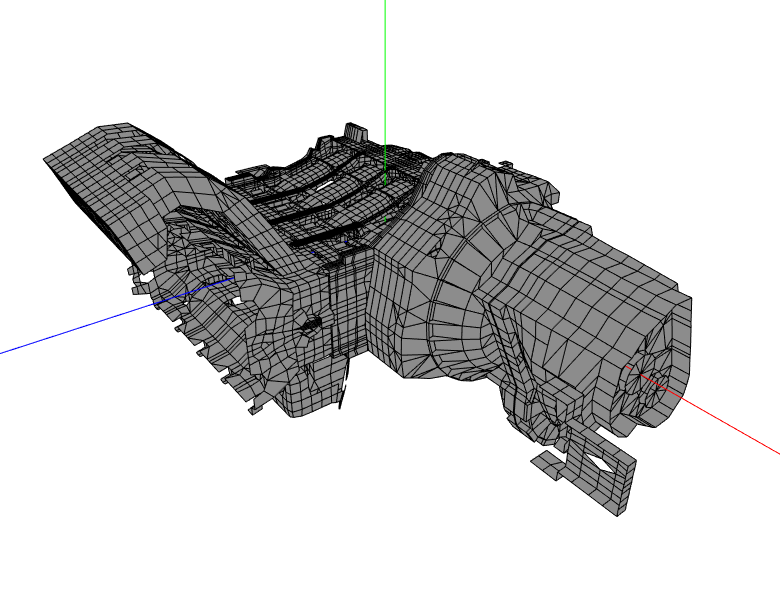
\includegraphics[width=\textwidth]{engine_default_color.png}
         \caption{Grafički međuspremnik koji je vidljiv korisniku}
         \label{fig:color-settings-normal-mode}
     \end{subfigure}
     \hfill
     \begin{subfigure}[h]{0.8\textwidth}
         \centering
         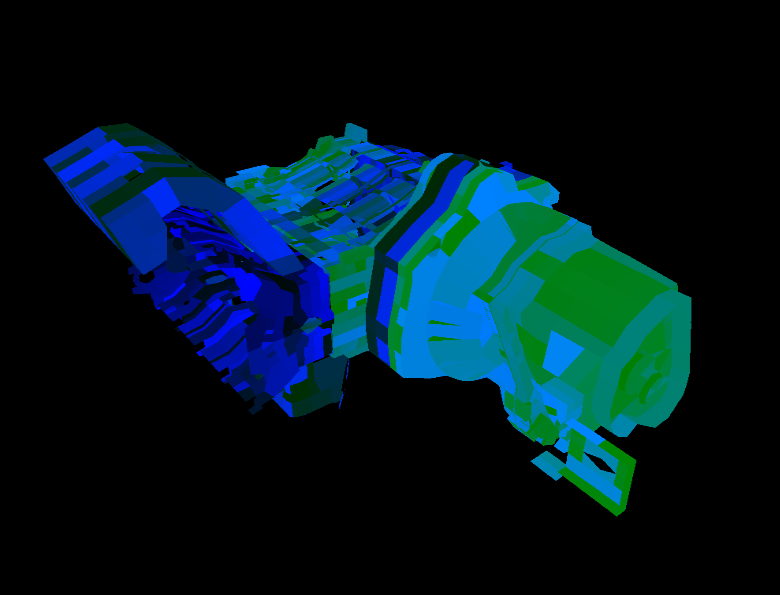
\includegraphics[width=\textwidth]{engine_cell_selection.png}
         \caption{Grafički međuspremnik za detekciju "lebdećeg" elementa}
         \label{fig:color-settings-limits-mode}
     \end{subfigure}
     \caption{Razlike između prikaza grafičkih međuspremnika}
     \label{fig:framebuffers-example}
\end{figure}

Druga klasa koja čini komponentu Pogleda je \textit{GraphManager}, a njena odgovornost je prikaz 2D grafova i legende gradijenta s obzirom na podatke koji su dostupni u Modelu poput: odabranih postavki, frekvencija i elemenata. Instanca ove klase izravno poziva metode biblioteke ImPlot koje su dodatno izmijenjene kako bi se omogućilo eksplicitno definiranje boja grafova i legende gradijenta preko argumenata metoda. Klasa se pretplaćuje na događaje i signale Modela koji su relevantni za ažuriranje instance pomoćne klase \textit{GraphData} unutar koje se čuvaju podaci važni za iscrtavanje grafova. Na ovaj način se objekt klase \textit{GraphData} ne mora ponovno "puniti" podacima u svakoj iteraciji petlje ažuriranja. No, \textit{GraphManager} izravno dohvaća podatke Modela (tj. ne pretplaćuje se na promjene) koji mijenjaju izgled grafa, ali ne zahtjevaju ponovno postavljanje objekta klase \textit{GraphData}. Konkretne metode iscrtavanja i uspoređivanja grafova te uzorkovanja legende gradijenta su implementirane pomoću obrasca Strategija, čime se olakšava potencijalno dodavanje novih metoda iste namjene. Za razliku od do sada objašnjenih klasa, klasa \textit{App} ne poziva direktno metodu za iscrtavanje grafova i legendi klase \textit{GraphManager}, već to radi klasa \textit{ImGuiManager} kada definira prozore korisničkog sučelja alata unutar kojih se te komponente trebaju nalaziti.\\

\subsection{Upravljač}

Komponenta Upravljač je u arhitekturi MVC odgovorna za komunikaciju s korisnikom, a kako je većina spomenute komunikacije u ovom alatu omogućena pomoću korisničkog sučelja koje pruža biblioteka Dear ImGui, glavna komponenta Upravljača je klasa \textit{ImGuiManager}. Navedena klasa je odgovorna za sve pozive metoda koje su dio biblioteke Dear ImGui, stoga ova klasa definira prozore korisničkog sučelja i njihove sadržaje, gumbe i funkcije koje se pozivaju na aktivaciju gumba, sučelja za mijenjanje boja i brojeva, izbornike i dijaloge za učitavanje datoteka itd. Budući da \textit{ImGuiManager} čuva pokazivače na instance klasa koje čine Model aplikacije, objekt ove klase omogućuje izravno mijenjanje dijelova Modela pomoću navedenih elemenata korisničkog sučelja. Osim navedenog, dužnost ove klase je i obavještavanje ostalih komponentama o događajima koji su vezani za korisničko sučelje poput promjene veličine prikaza motora ili definiranje direktorija datoteke za učitavanje podataka o motoru. Instanca ove klase čuva pokazivač na objekt klase \textit{MeshManager} kako bi pristupila teksturi u koju je spremljen grafički međuspremnik koji se prikazuje korisniku (opisan u poglavlju \ref{view-section}). Spomenutu teksturu zatim može prikazati u prozoru zaduženom za prikaz motora. Uz to instanca klase \textit{ImGuiManager} čuva i pokazivač na objekt klase \textit{GraphManager} čije metode koristi za iscrtavanje grafova i legende gradijenta.\\

Važno je naglasiti kako, unatoč tome što je veliki dio interakcije s korisnikom u alatu implementiran pomoću biblioteke Dear ImGui, veliki dio stvarne interakcije koju korisnik obavlja s alatom nije vezan za dijelove korisničkog sučelja već za događaje poput klika i kretanja miša, te pomicanja kotačića miša. Ti su događaji važni kako bi se korisniku omogućilo označavanje i odabiranje "lebdećeg" elementa te kontrola kamere. Kako je već spomenuto na početku poglavlja \ref{codebase-architecture-section}, klasa \textit{App} zapravo obrađuje GLFW događaje koji javljaju ovakav tip korisničkog unosa. Budući da su takvi događaji \textit{ImGuiManager}-u važni za obraditi, objekt klase \textit{App} prvo pozove metodu objekta klase \textit{ImGuiManager} koja je zadužena za obrađivanje specifičnog događaja. U spomenutoj metodi se obrađivanje događaja delegira biblioteci Dear ImGui, a zatim se ispita je li pokazivač miša iznad prikaza modela motora, pošto su sve navedene interakcije vezane za prikaz modela motora. \textit{ImGuiManager} vraća odgovor na taj upit preko povratne vrijednosti pozvane funkcije. Ako je pokazivač miša iznad prikaza motora u trenutku pojave događaja, objekt klase \textit{App} će događaj dodatno obraditi pomoću ostalih komponenti MVC arhitekture, tako da je na neizravan način i klasa \textit{App} dio komponente Upravljač.


\section{Organizacija podataka na grafičkoj kartici} \label{graphics-card-data-section}

U poglavlju \ref{view-section} je objašnjeno kako četiri klase šalju vlastitim sjenčarima različite podatke na grafičku karticu jer imaju različite uloge. Cilj ovog poglavlja je detaljnije objašnjavanje toka podataka između procesora i grafičke kartice za svaku od navedenih klasa, a kako bi se omogućilo što razumljivije objašnjavanje tog toka, važno je objasniti nekoliko generalnih razlika između načina slanja i iscrtavanja podataka korištenih u ovom alatu.\\

U alatu razvijenom u sklopu ovog rada se podaci na grafičku karticu šalju na dva načina: pomoću  \textit{vertex buffer object}-a i pomoću uniformnih varijabli. \textit{Vertex buffer object}-i (skraćeno VBO) sadrže polje podataka koji opisuju svaki vrh modela na način koji je relavantan sjenčaru vrhova. U grafičkom protočnom sustavu sjenčar vrhova procesira elemente VBO-a, a rezultate prosljeđuje u daljnji dio protočnog sustava. Za jedan sjenčar se može definirati proizvoljan broj VBO-a samo je važno uvijek povezati strukturu elementa koji je sačuvan u VBO-u s atributima sjenčara vrhova pomoću funkcija OpenGL-a poput \textit{glVertexAttribPointer}. Uniformne varijable su iste za svaki vrh, te su zajedničke sjenčaru vrhova i sjenčaru fragmenata. Njih klijent ne šalje na grafičku karticu učitavanjem u VBO-e, već izravnim definiranjem lokacije i "pakirane "vrijednosti uniformne varijable. Klijent saznaje lokaciju uniformne varijable u sjenčaru pozivanjem funkcije \textit{glGetUniformLocation} kojoj kao argumente predaje indeks sjenčara i ime uniformne varijable.\\

Također, u alatu se koriste i dvije različite metode za iscrtavanje podataka učitanih u VBO: \textit{glDrawArrays} i \textit{glDrawElements}. Metoda \textit{glDrawArrays} svaki element VBO-a šalje jednom u sjenčar vrhova, te pretpostavlja da su vrhovi unutar VBO-a poredani slijedno i prate strukturu koju predstavljaju, npr. tri vrha iz istog trokuta su unutar VBO-a definirani jedan za drugim, te zadnji trokut neće imati broj vrhova koji nije djeljiv s tri. S druge strane metoda \textit{glDrawElements} zahtjeva dodatno definirani \textit{buffer object} zvani \textit{element buffer object} (skraćeno EBO) unutar kojeg su spremljeni indeksi podataka iz VBO-a koji definiraju poredak iscrtavanja učitanih podataka. Korištenjem ove metode u slučaju kada lica modela imaju velik broj dijeljenih vrhova, značajno se smanjuje broj podataka koji se šalje preko VBO-a jer se podaci ponavljajućih vrhova mogu "reciklirati" višestrukim navođenjem indeksa tog vrha unutar EBO-a.

\subsection{Podaci za bojanje elemenata}

Podaci koji su relevantni za bojanje elemenata su organizirani u dva VBO-a i 4 uniformne varijable. Preko VBO-a, tj. podataka koji opisuju pojedini vrh, se šalju pozicije vrhova, indeks elementa kojem pripadaju i boja tog elementa. Ti podaci su rastavljeni u dva VBO-a tako da se pozicija vrha i indeks elementa kojem taj vrh pripada šalju u sklopu jednog VBO-a, a boja vrha pomoću drugog. Na taj način se podaci koji su konstantni (pozicija vrha i indeks elementa) ne moraju slati svaki put kada se mijenjaju boje modela motora, već se šalju samo kada se učitaju iz datoteka.\\

Uniformne varijable koje se šalju na karticu za potrebe bojanja elemenata su matrice modela, pogleda i projekcije, te indeks trenutnog "lebdećeg" elementa. Matrica modela je konstantno postavljena na matricu identiteta, a matrice pogleda i projekcije su tu kako bi se model pravilno iscrtavao i nakon promjene rotacije i pozicije kamere, te promjene dimenzija prozora prikaza motora. Indeks trenutnog "lebdećeg" elementa je poslan kako bi sjenčar znao kojem elementu treba postaviti boju na inverz trenutne boje. Na taj način nije potrebno ažurirati VBO s bojama elemenata svaki put kada pokazivač miša bude postavljen na novi element.\\

Za iscrtavanje ovih podataka se koristi metoda \textit{glDrawElements}, tako da je uz slanje podataka, potrebno poslati i indekse koji definiraju po kojem poretku se ti podaci isrtavaju. Iako se na prvi pogled može primjetiti kako elementi međusobno ne dijele vrhove jer vrhovi imaju podatak o elementu kojem pripadaju, važno je napomenuti kako OpenGL u \textit{core} načinu rada samo podržava iscrtavanje trokuta. Stoga četverokutne elemente treba podijeliti na trokute, pa korištenjem metode \textit{glDrawElements}, ti elementi ne šalju više šest točaka unutar VBO-a, već četiri. Budući da takvi elementi čine ukupno 90.191\% svih elemenata modela motora koji se koristi u ovom radu (ostatak elemenata su trokuti), primjenom ove optimizacije se na grafičku karticu šalje 31.614\% manje podataka o vrhovima.

\subsection{Podaci za detekciju lebdećeg elementa}

Podaci koji se koriste za iscrtavanje motora s elementima jedinstvenih boja (opisano u poglavlju \ref{view-section}) se na grafičku karticu šalju pomoću jednog VBO-a koji za svaki vrh definira njegovu poziciju i indeks elementa kojem pripada, te pomoću tri uniformne varijable: matrica modela, pogleda i projekcije. Sjenčar iz indeksa elementa izračuna boju vrha tog elementa, a klasa \textit{EngineCellSelectionMesh} obavlja inverznu operaciju nakon što uzorkuje boju na pikselu iznad kojeg je postavljen pokazivač miša. Za ovo iscrtavanje se također koristi metoda \textit{glDrawElements}, te je smanjenje broja podataka jednako kao i kod podataka za bojanje elemenata.

\subsection{Podaci za linije elemenata}

Podaci koji se koriste za crtanje linija između elemenata se na grafičku karticu šalju pomoću jednog VBO-a koji prenosi samo pozicije vrhova linija i tri uniformne varijable koje su matrice modela, pogleda i projekcije. Ovi podaci se također iscrtavaju pomoću metode \textit{glDrawElements} od koje dobivaju veću uštedu u odnosu na korištenje metode \textit{glDrawArrays} jer se pozicije vrhova mogu dijeliti između elemenata.

\subsection{Podaci za koordinatne osi}
Za crtanje linija koordinatnih osi se koristi jedan VBO unutar kojeg se prenosi polje podataka o vrhovima koji su opisani u dva bajta: prvi bajt je indeks u rasponu od 0 do 3, te služi za identificiranje pozicije vrha koordinatnih osi (točka ishodišta ili vrh x/y/z osi), a drugi bajt je indeks u rasponu od 0 do 2 i definira kojoj osi taj vrh pripada. Sjenčar interno definira konstantna polja koja indeksira pomoću indeksa iz VBO-a. Osim VBO-a sjenčar prima i dvije uniformne varijable: matrice pogleda i projekcije. Za razliku od dosadašnjih podataka, ovi podaci se crtaju metodom \textit{glDrawArrays}. Ova metoda se koristi zbog jednostavnosti i manje količine potrebnih podataka u odnosu na metodu \textit{glDrawElements}, koja bi zahtijevala dodatno definiranje EBO-a, što za ovako mali broj vrhova nema smisla.

\chapter{Demonstracija rada alata}

\section{Učitavanje datoteka}

Kada korisnik prvi put pokrene alat, prozori alata će izgledati slično kao na slici \ref{fig:initial-screenshot}. Važno je naglasiti kako korisnik može promijeniti poziciju i veličinu svakog prozora u sklopu alata, a ta promjena će ostati spremljena nakon zatvaranja alata.

\begin{figure} [H]
	\centering
    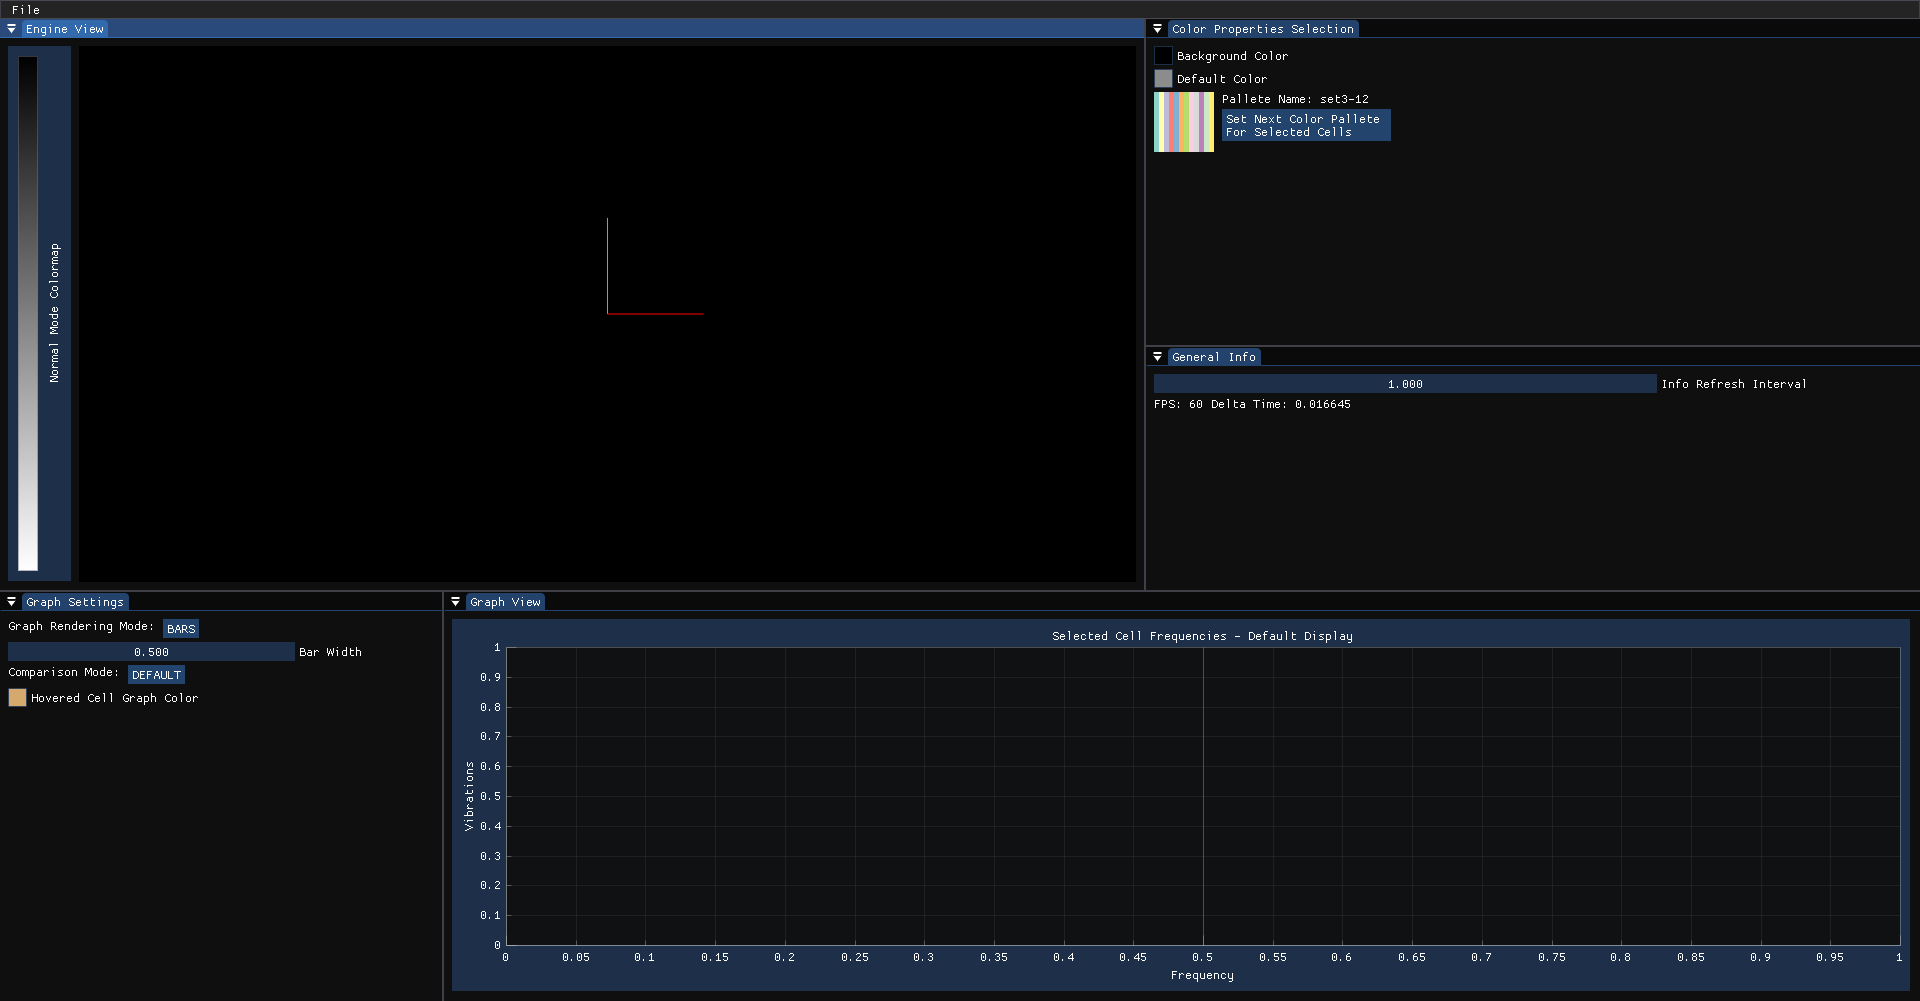
\includegraphics[width=\textwidth]{demonstration/initial_screenshot.png}
    \caption{Prikaz alata nakon pokretanja}
    \label{fig:initial-screenshot}
\end{figure}

Kako bi korisnik mogao vizualizirati podatke s kojima su vibracije elemenata opisane, potrebno ih je učitati iz datoteka pomoću prikazanog na slici \ref{fig:file-menu}. Klikom na bilo koji gumb tog izbornika se otvara dijalog za odabiranje datoteka prikazan na slici \ref{fig:file-dialog}.

\begin{figure} [H]
	\centering
    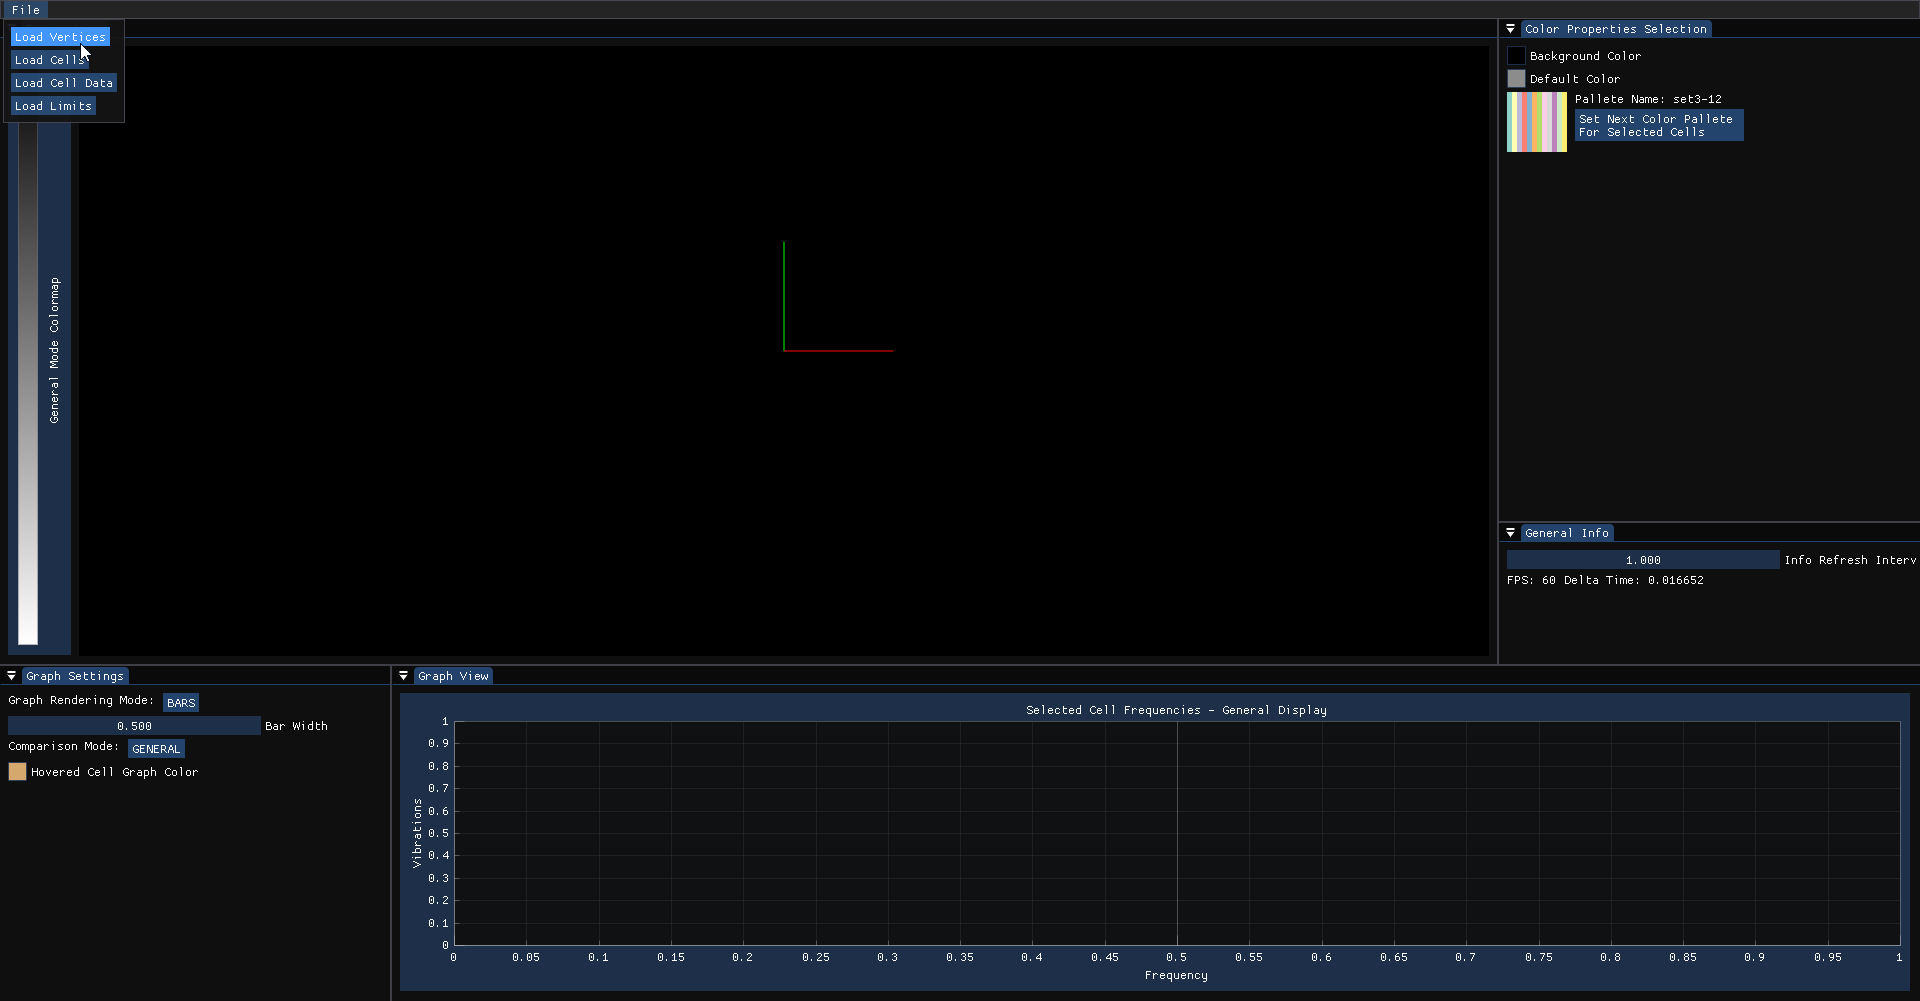
\includegraphics[width=\textwidth]{demonstration/load_file_menu.png}
    \caption{Izbornik za učitavanje datoteka}
    \label{fig:file-menu}
\end{figure}

\begin{figure} [H]
	\centering
    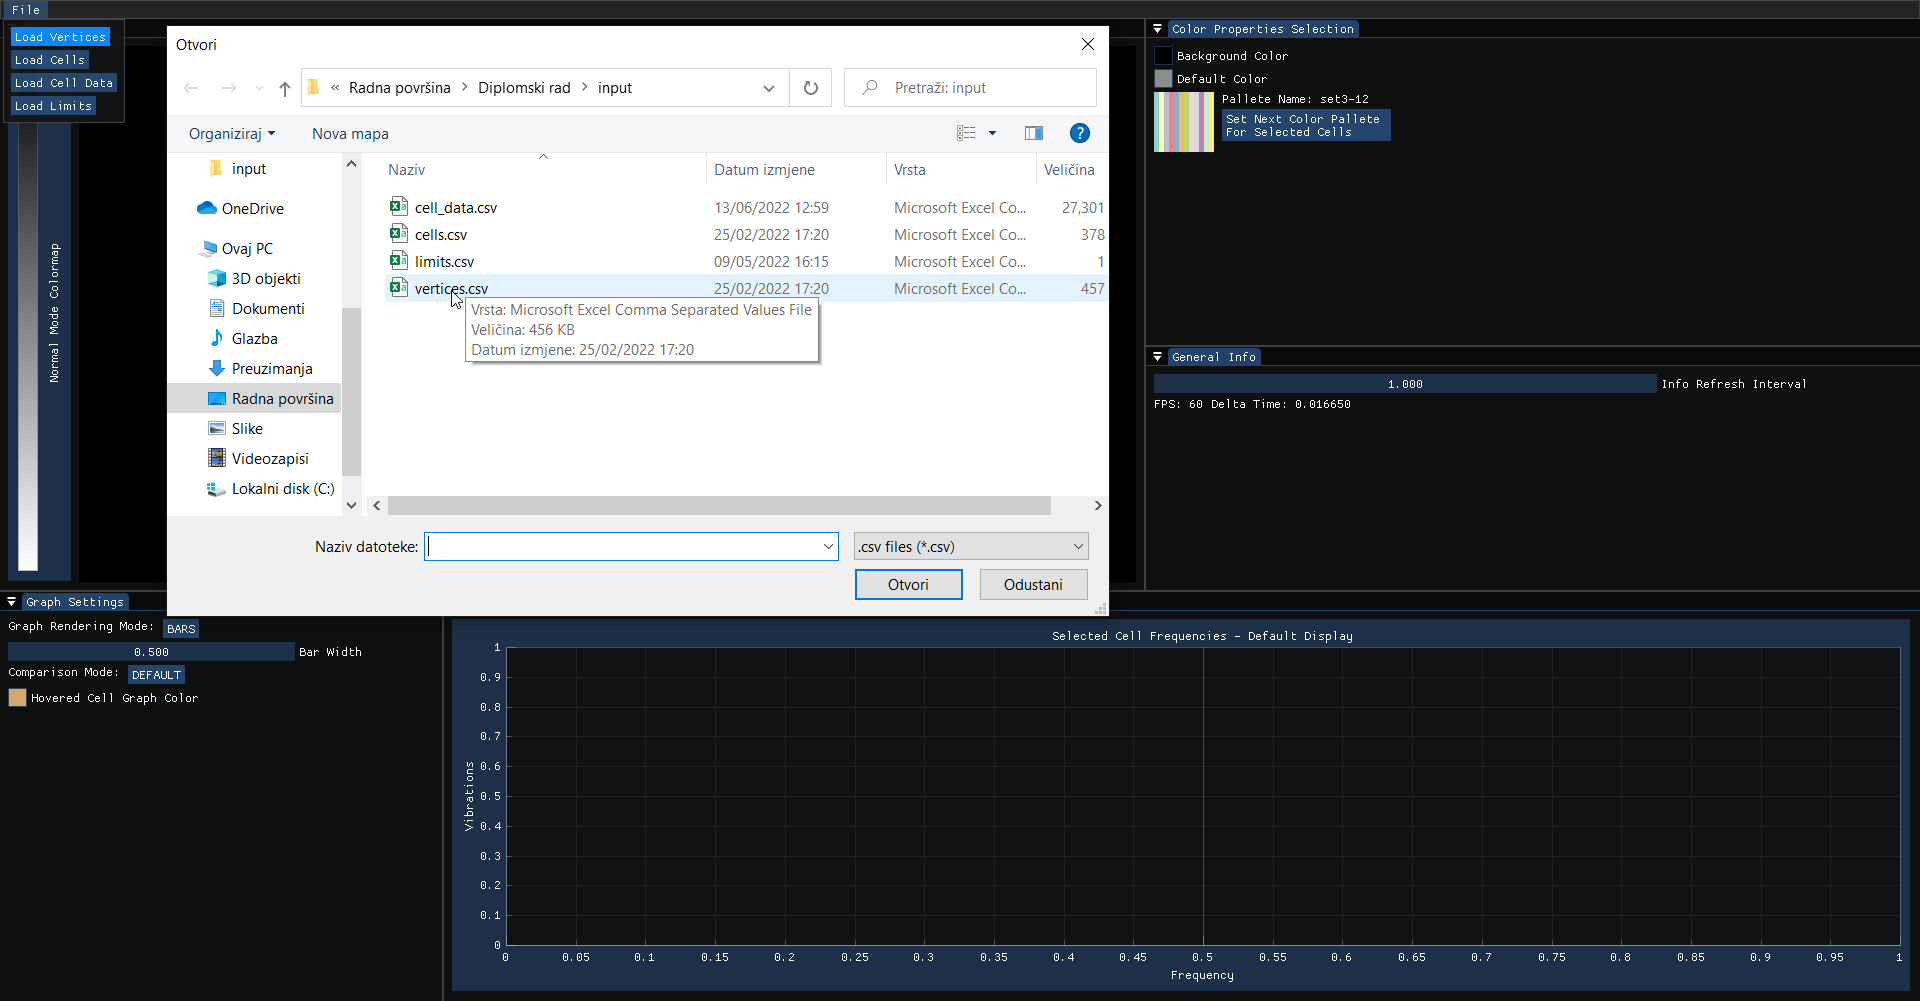
\includegraphics[width=\textwidth]{demonstration/file_select_dialog.png}
    \caption{Dijalog za odabiranje datoteke}
    \label{fig:file-dialog}
\end{figure}

Nakon što su sve datoteke učitane, izgled alata bi trebao sličiti prikazu sa slike \ref{fig:loaded-files-tool}.

\begin{figure} [H]
	\centering
    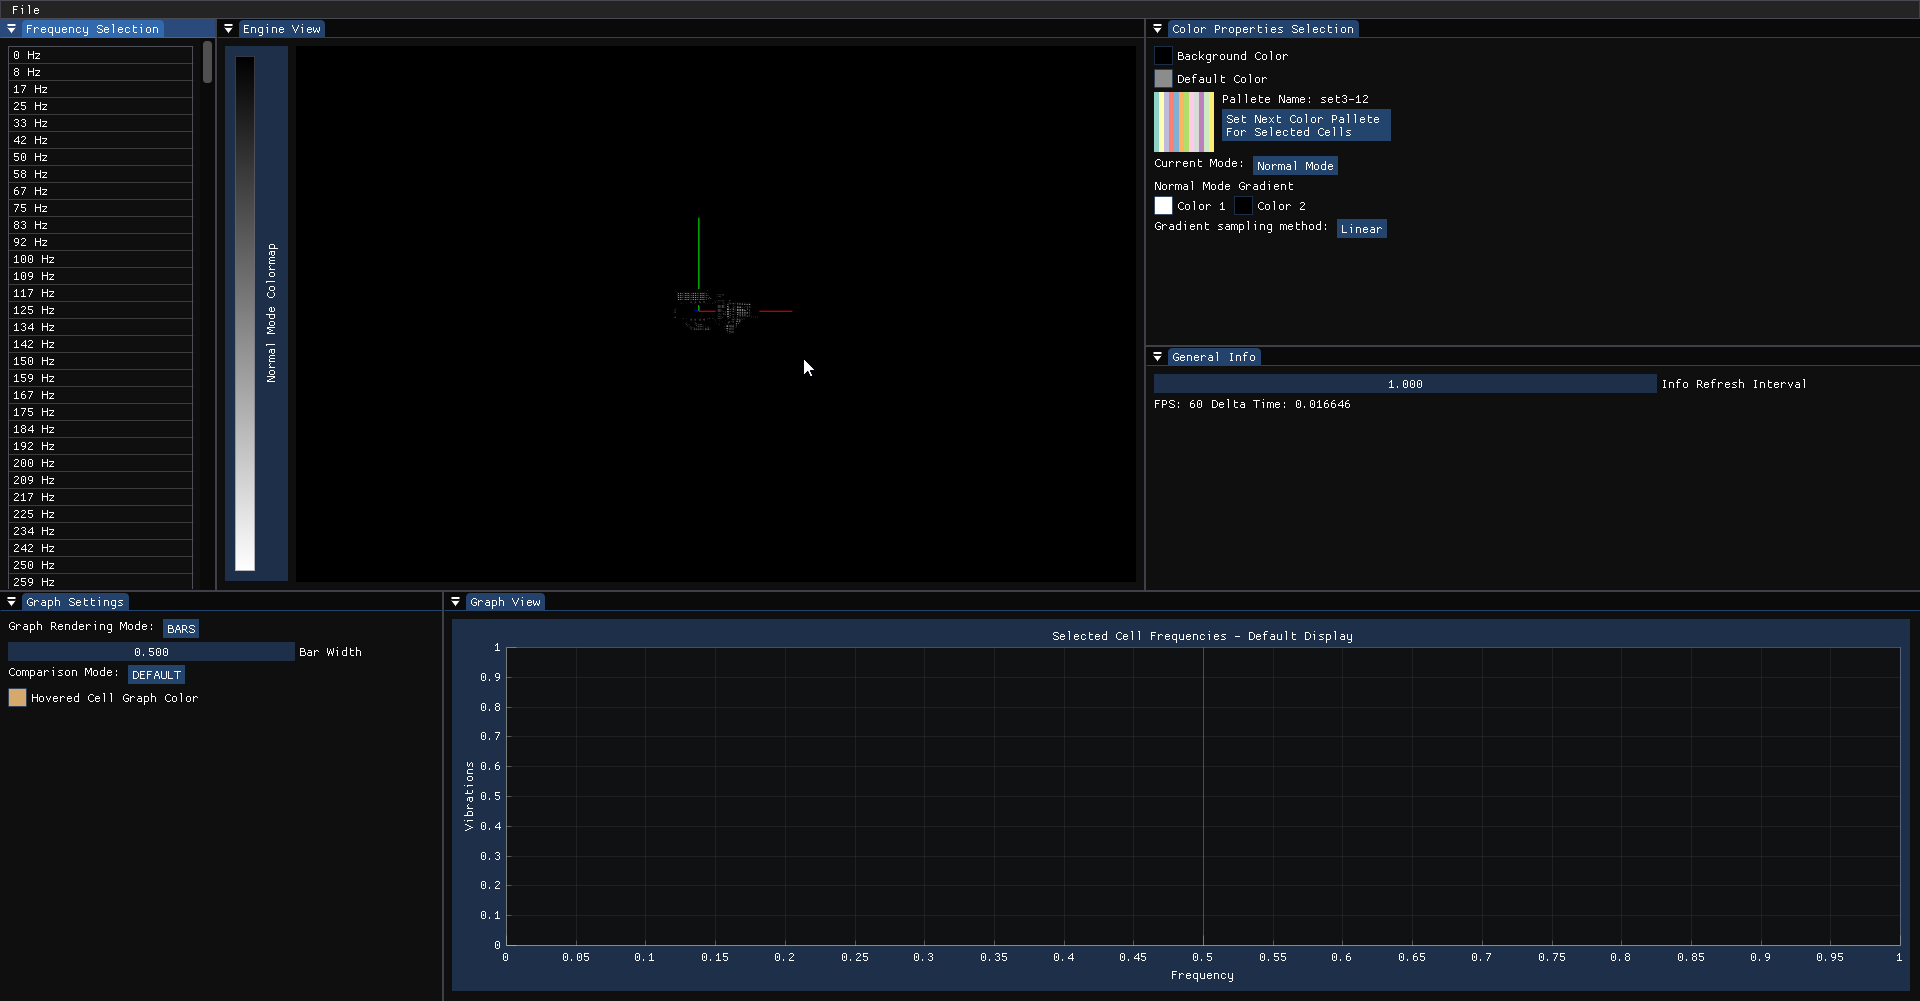
\includegraphics[width=\textwidth]{demonstration/files_loaded_screenshot.png}
    \caption{Prikaz alata nakon što su sve relevantne datoteke učitane}
    \label{fig:loaded-files-tool}
\end{figure}

\section{Općenita analiza vibracija}

Alat u početku koristi općenitu analizu vibracija. U prikazu alata sa slike \ref{fig:loaded-files-tool} korisnik može odabrati frekvencije vibriranja za koje ga zanima snaga vibracije elemenata motora, na što se boje elemenata motora ažuriraju slično kao na slici \ref{fig:selected-frq}.

\begin{figure} [H]
	\centering
    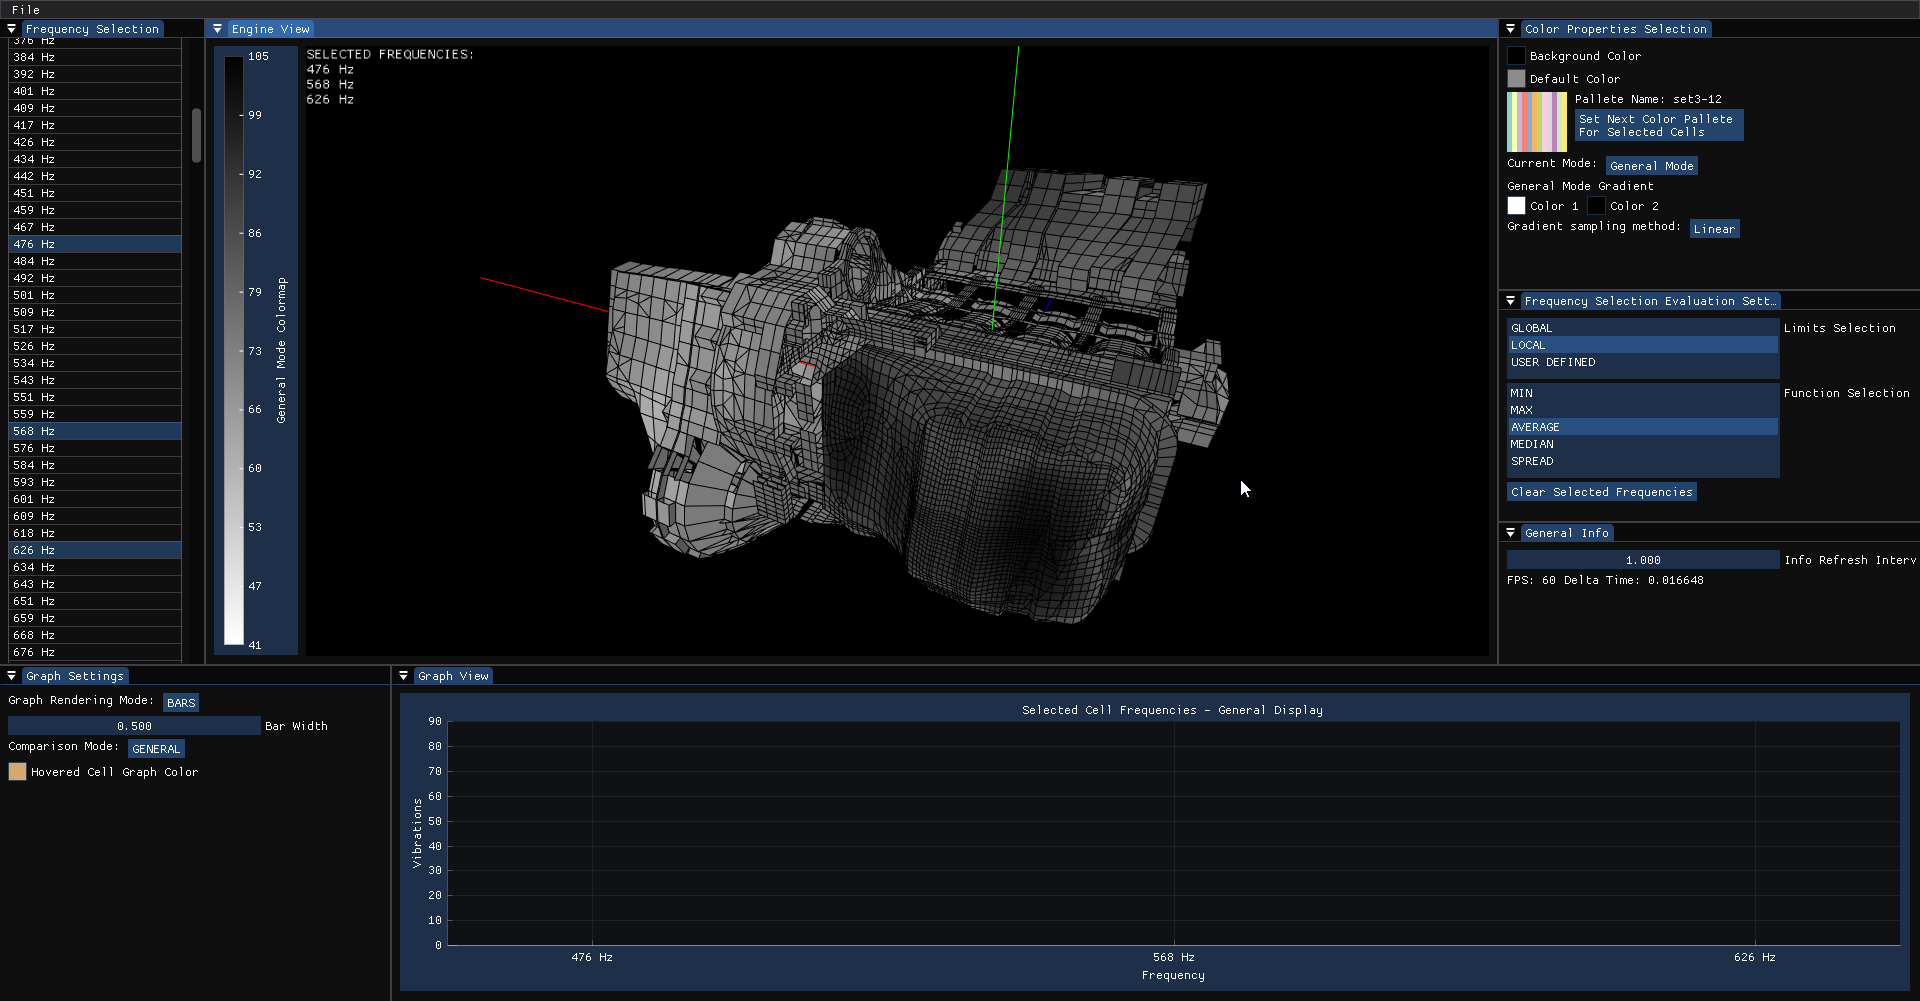
\includegraphics[width=\textwidth]{demonstration/selected_frq.png}
    \caption{Odabiranje frekvencija u općenitoj analizi vibracija}
    \label{fig:selected-frq}
\end{figure}

Ako korisniku vidljivost ili izgled početno postavljenog gradijenta ne odgovara, moguće je promijeniti boje koje opisuju gradijent, kao što je prikazano na slici \ref{fig:color-select}.

\begin{figure} [H]
	\centering
    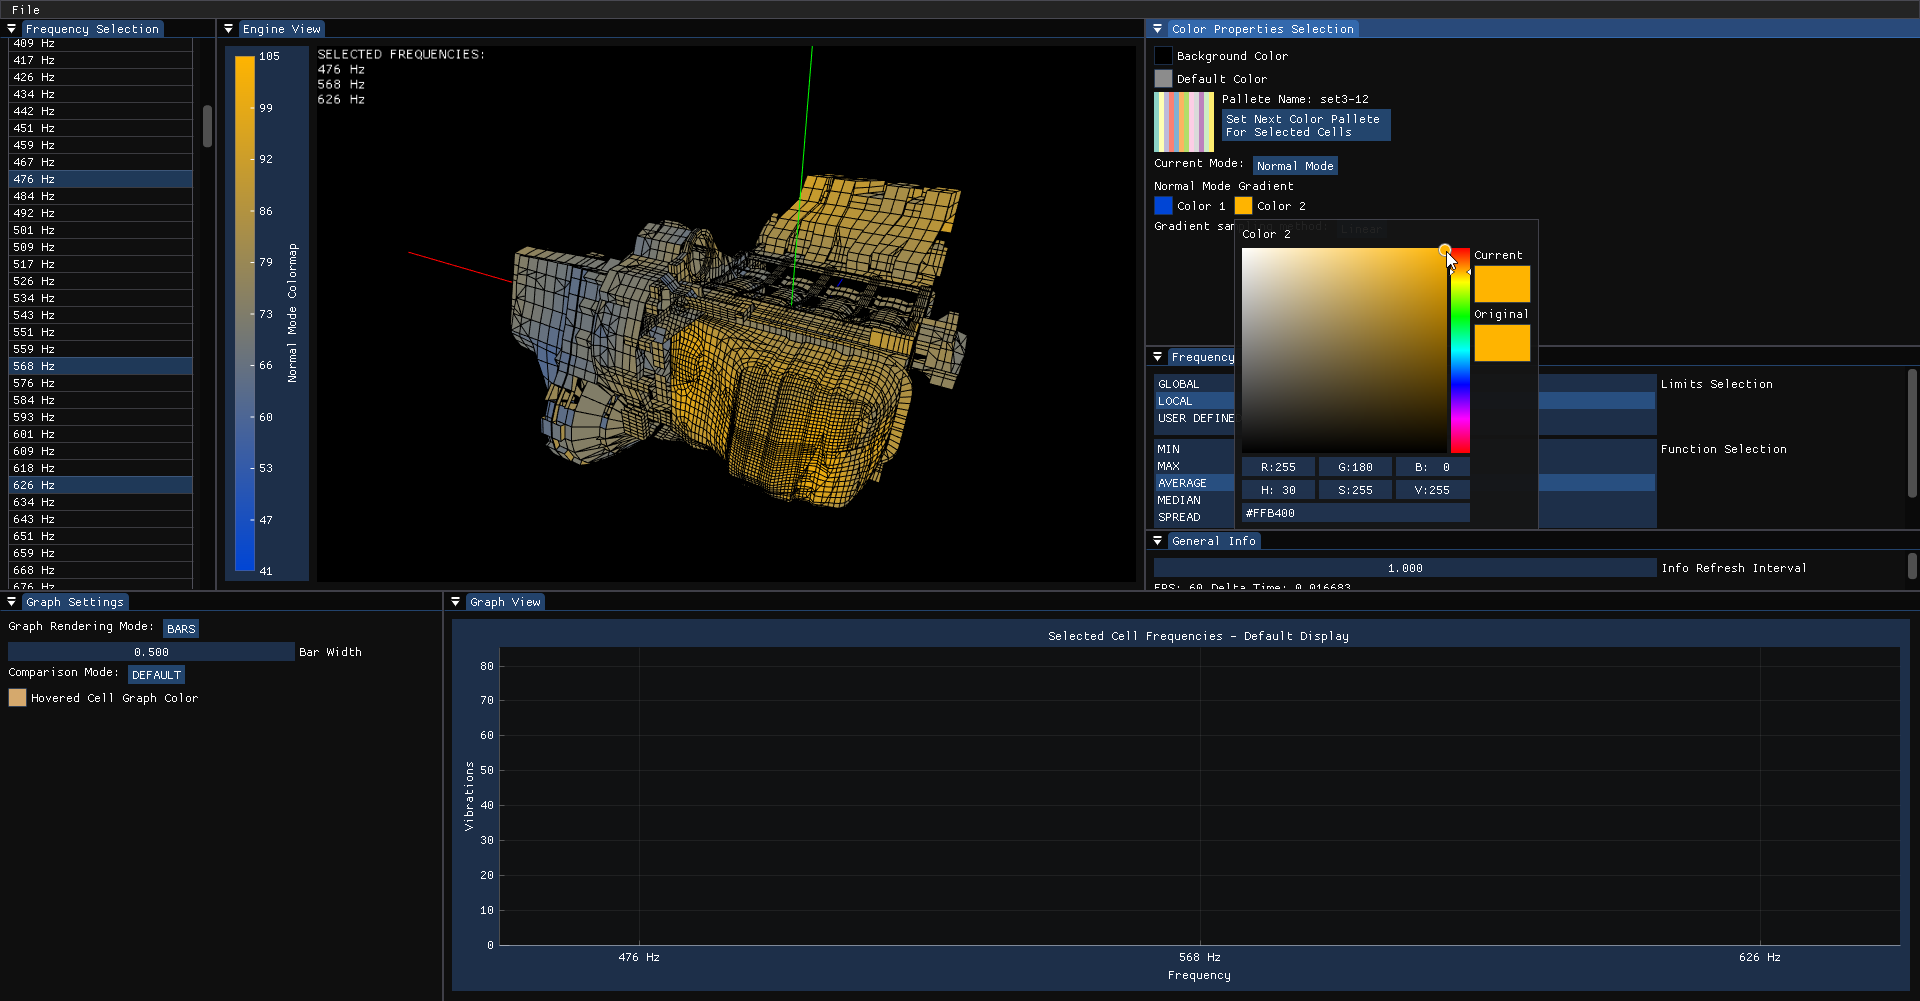
\includegraphics[width=\textwidth]{demonstration/color_select.png}
    \caption{Odabiranje boja gradijenta}
    \label{fig:color-select}
\end{figure}

No, sa slike \ref{fig:color-select} je vidljivo kako boja koja označava vibracije pri vrhu lokalnog raspona zauzima nešto manje od pola gradijenta, što korisniku vjerojatno nije pretjerano korisno ako želi uočiti kritične dijelove motora. Iz tog razloga, korisnik može promijeniti način uzorkovanja gradijenta, a na slici \ref{fig:quartic-engine-colors} se može vidjeti kako kvartičko uzorkovanje uvelike pomaže pri vizualnom izoliranju ekstrema.

\begin{figure} [H]
	\centering
    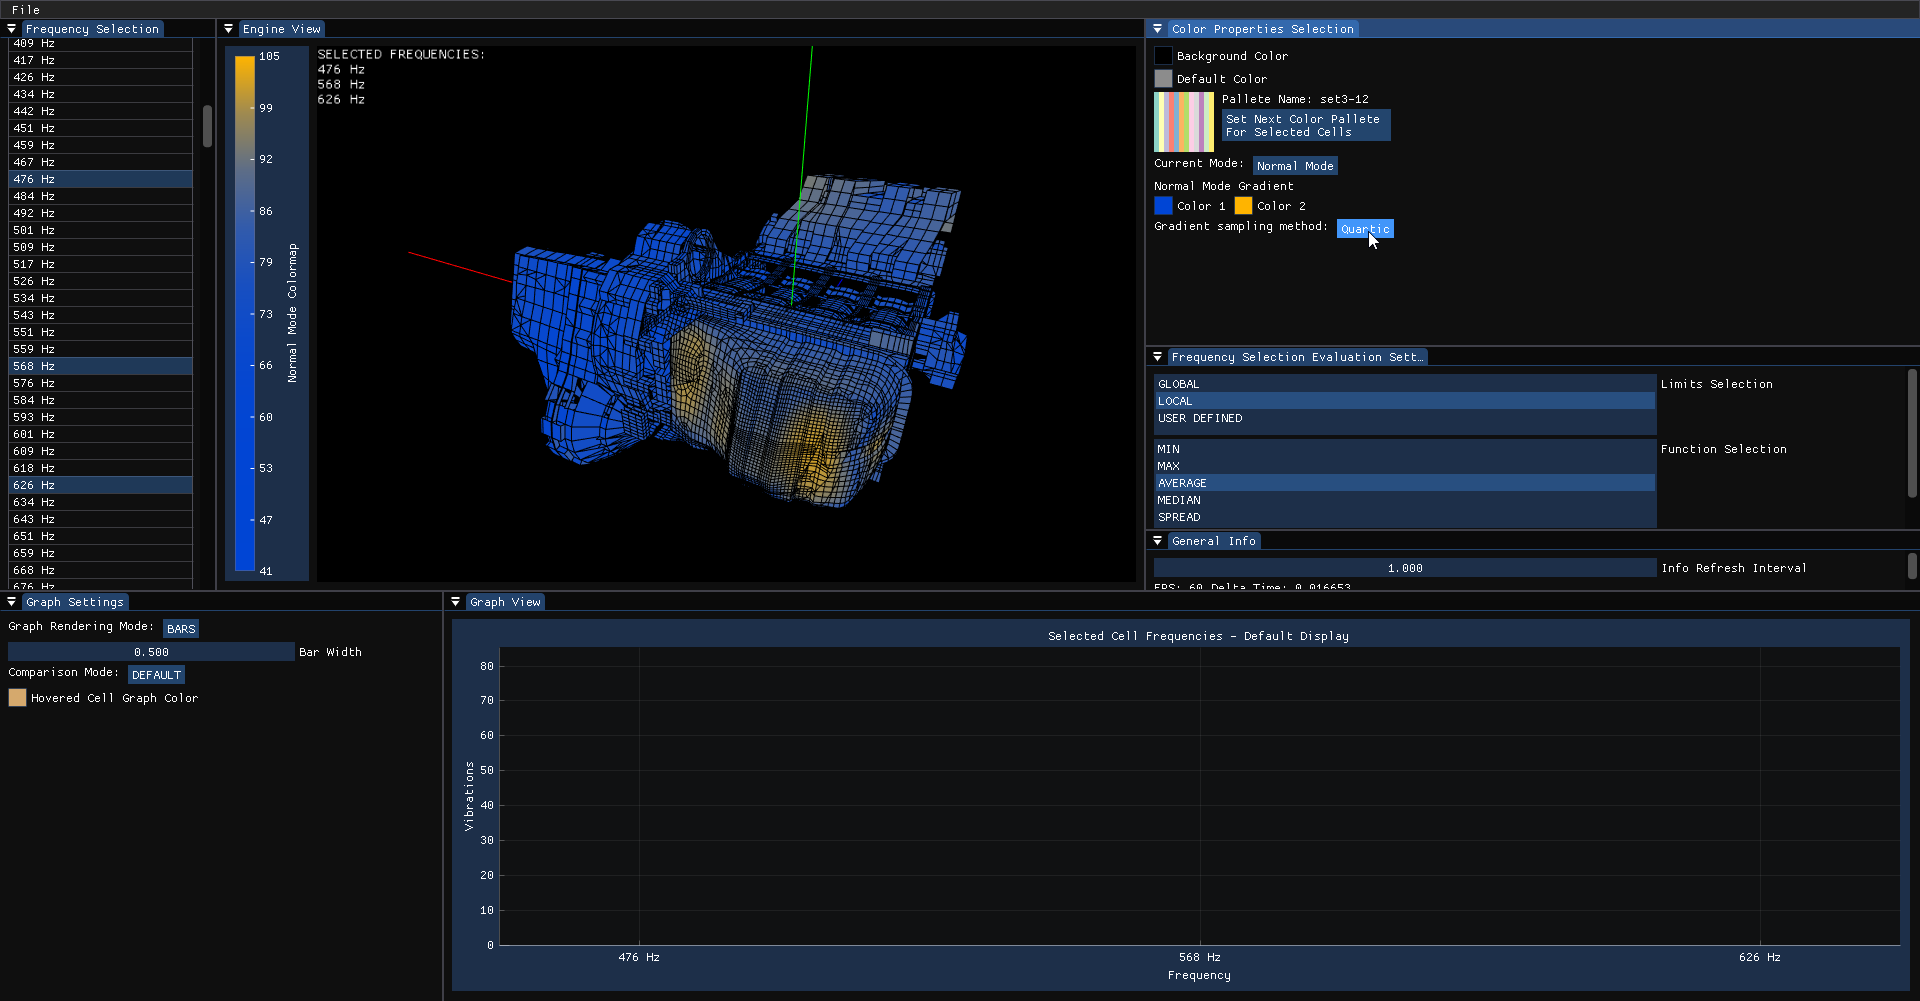
\includegraphics[width=\textwidth]{demonstration/quartic_sampling_normal_mode.png}
    \caption{Boje elemenata motora pri kvartičkom uzorkovanju gradijenta}
    \label{fig:quartic-engine-colors}
\end{figure}

Ako korisnik želi veću kontrolu nad isticanjem ekstremnih vrijednosti, može to učiniti "ručnim" definiranjem raspona. Na ovakav način korisnik može definirati proizvoljni minimum i maksimum ekstremnih vrijednosti. No, važno je naglasiti kako je pri ovakvom načinu izoliranja ekstrema dobro koristiti linearno uzorkovanje gradijenta jer ostala uzorkovanja najvjerojatnije neće "kritičnom" bojom obojati većinu elemenata koji pripadaju rasponu ekstremnih vrijednosti kojeg je korisnik definirao. Na slici \ref{fig:custom-interval} se može vidjeti primjer korištenja intervala definiranog od strane korisnika. Na spomenutoj slici se također koristi i funkcija MAX, koja je korisna ako korisnika zanima koliko će najjače element vibrirati pri odabranim frekvencijama.

\begin{figure} [H]
	\centering
    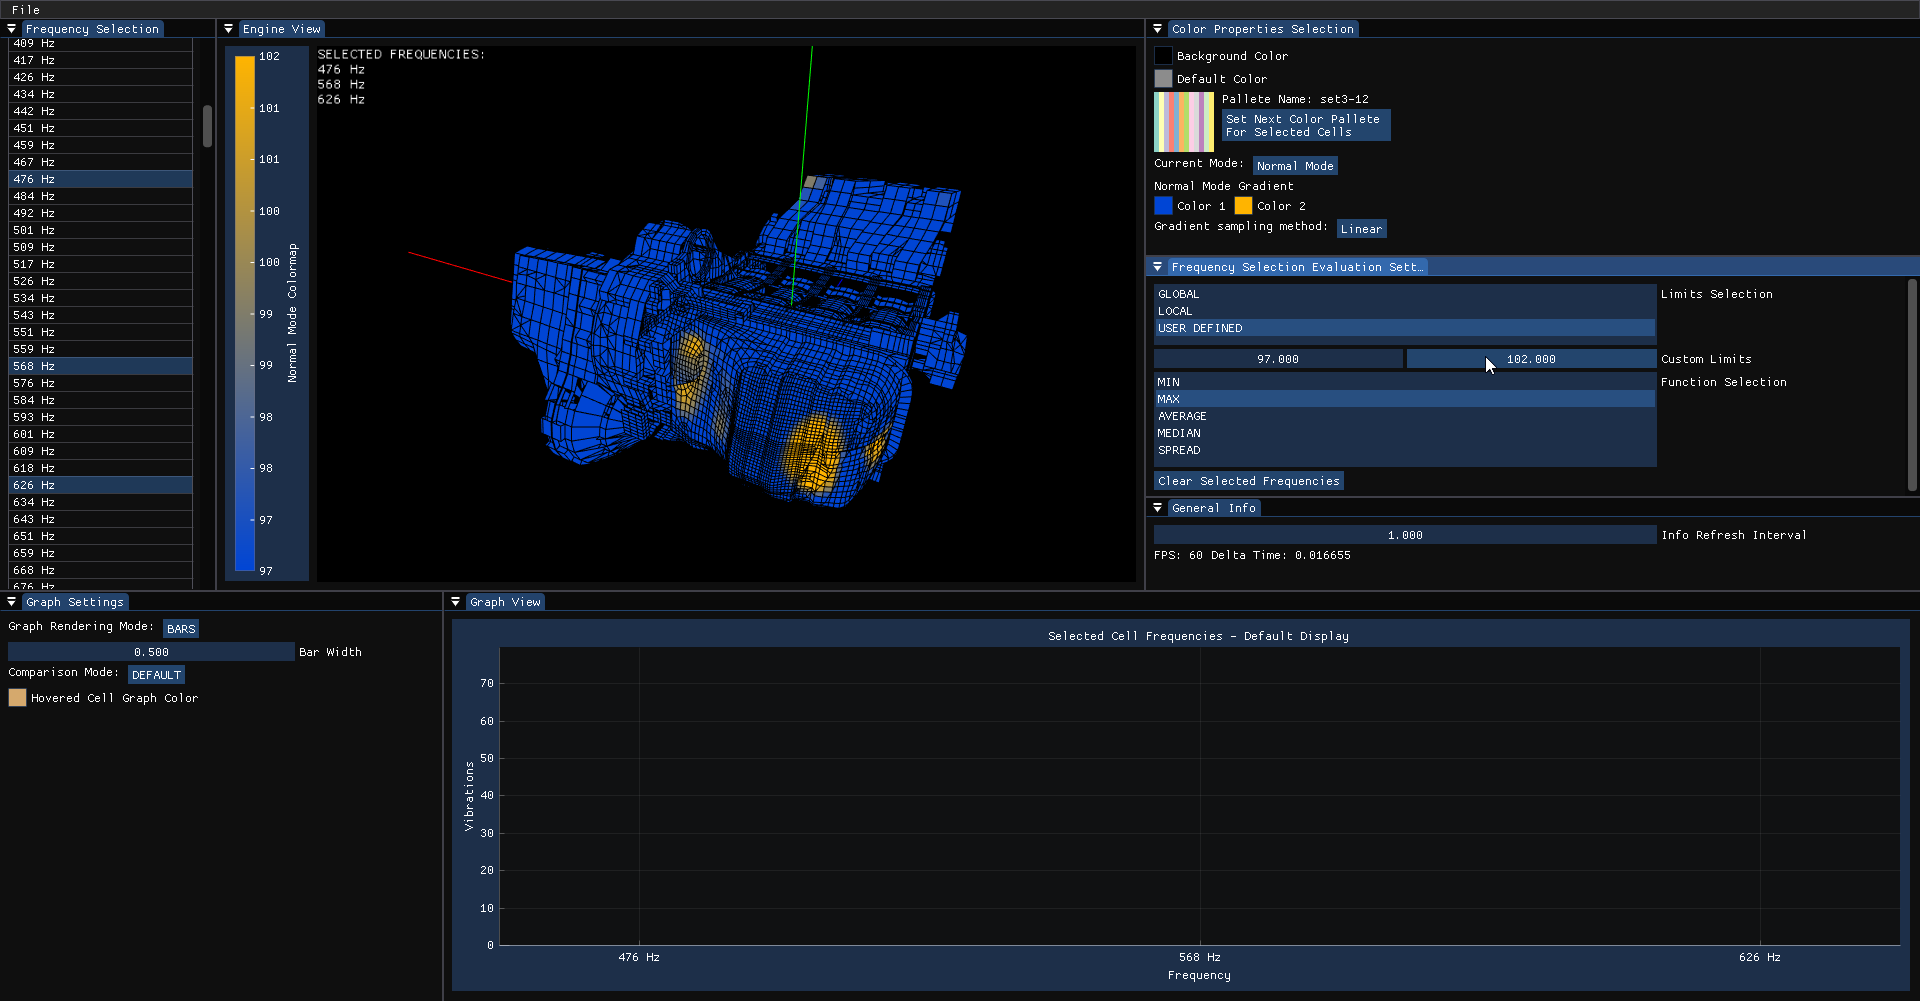
\includegraphics[width=\textwidth]{demonstration/custom_limits_linear_sampling.png}
    \caption{Izgled motora uz "ručno" definirani raspon i korištenje funkcije MAX}
    \label{fig:custom-interval}
\end{figure}

"Ručno" definiranje raspona također može biti korisno i kod korištenja funkcije SPREAD. Izgled motora prilikom korištenja te funkcije je vidljiv na slici \ref{fig:spread-view}. Navedena funkcija vraća razliku između najveće i najmanje snage vibracije elementa pri odabranim frekvencijama, pa se korištenjem ove funkcije uz raspon definiran od strane korisnika može preciznije definirati interval razlika u snazi vibriranja elementa koji je korisniku bitan za uočiti. 

\begin{figure} [H]
	\centering
    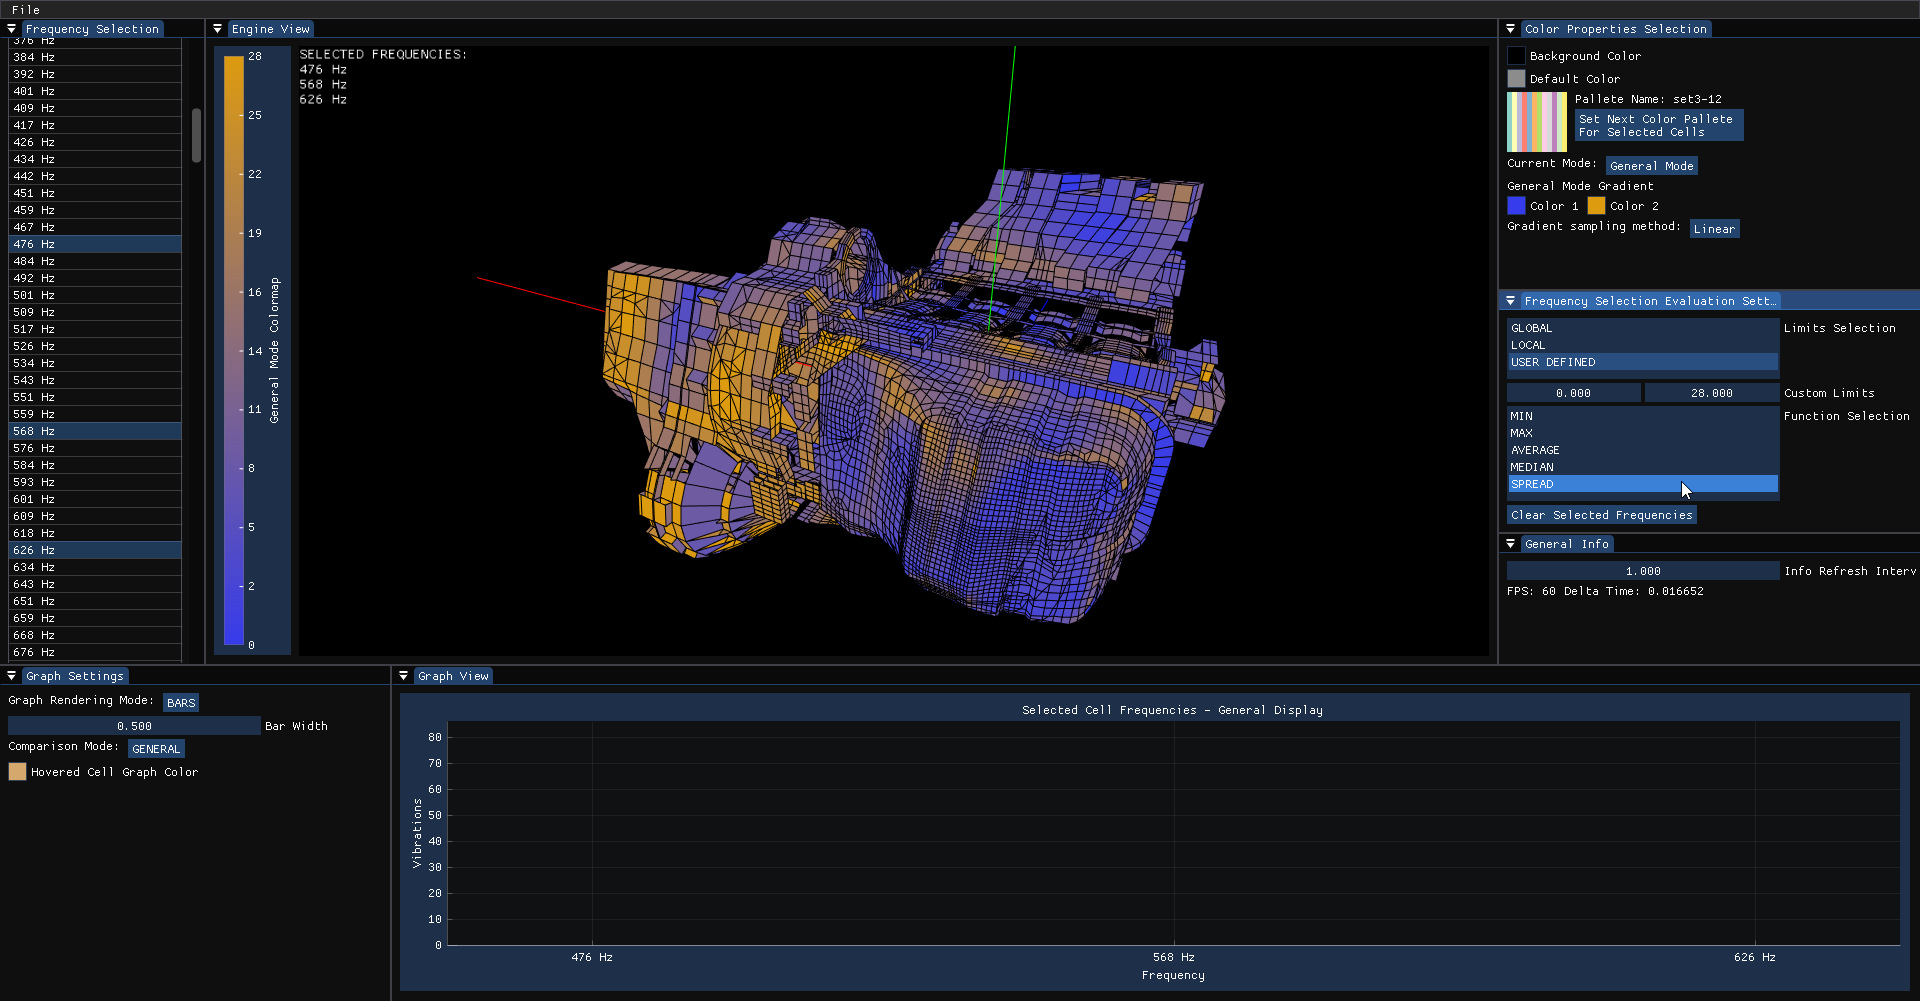
\includegraphics[width=\textwidth]{demonstration/spread.png}
    \caption{Izgled motora pri korištenju funkcije SPREAD uz raspon koji je definiran od strane korisnika}
    \label{fig:spread-view}
\end{figure}

\section{Analiza vibracija s preddefiniranim ograničenjima}

Klikom na gumb s imenom trenutne vrste analize, alat prelazi iz općenite analize u analizu s preddefiniranim ograničenjima i obratno. Na slici \ref{fig:limits-mode-switched} se može vidjeti kako je broj frekvencija koje se može odabrati u analizi s preddefiniranim ograničenjima puno manji nego u općenitoj analizi jer su samo dostupne frekvencije za koje su ograničenja definirana u datoteci iz koje su učitana.

\begin{figure} [H]
	\centering
    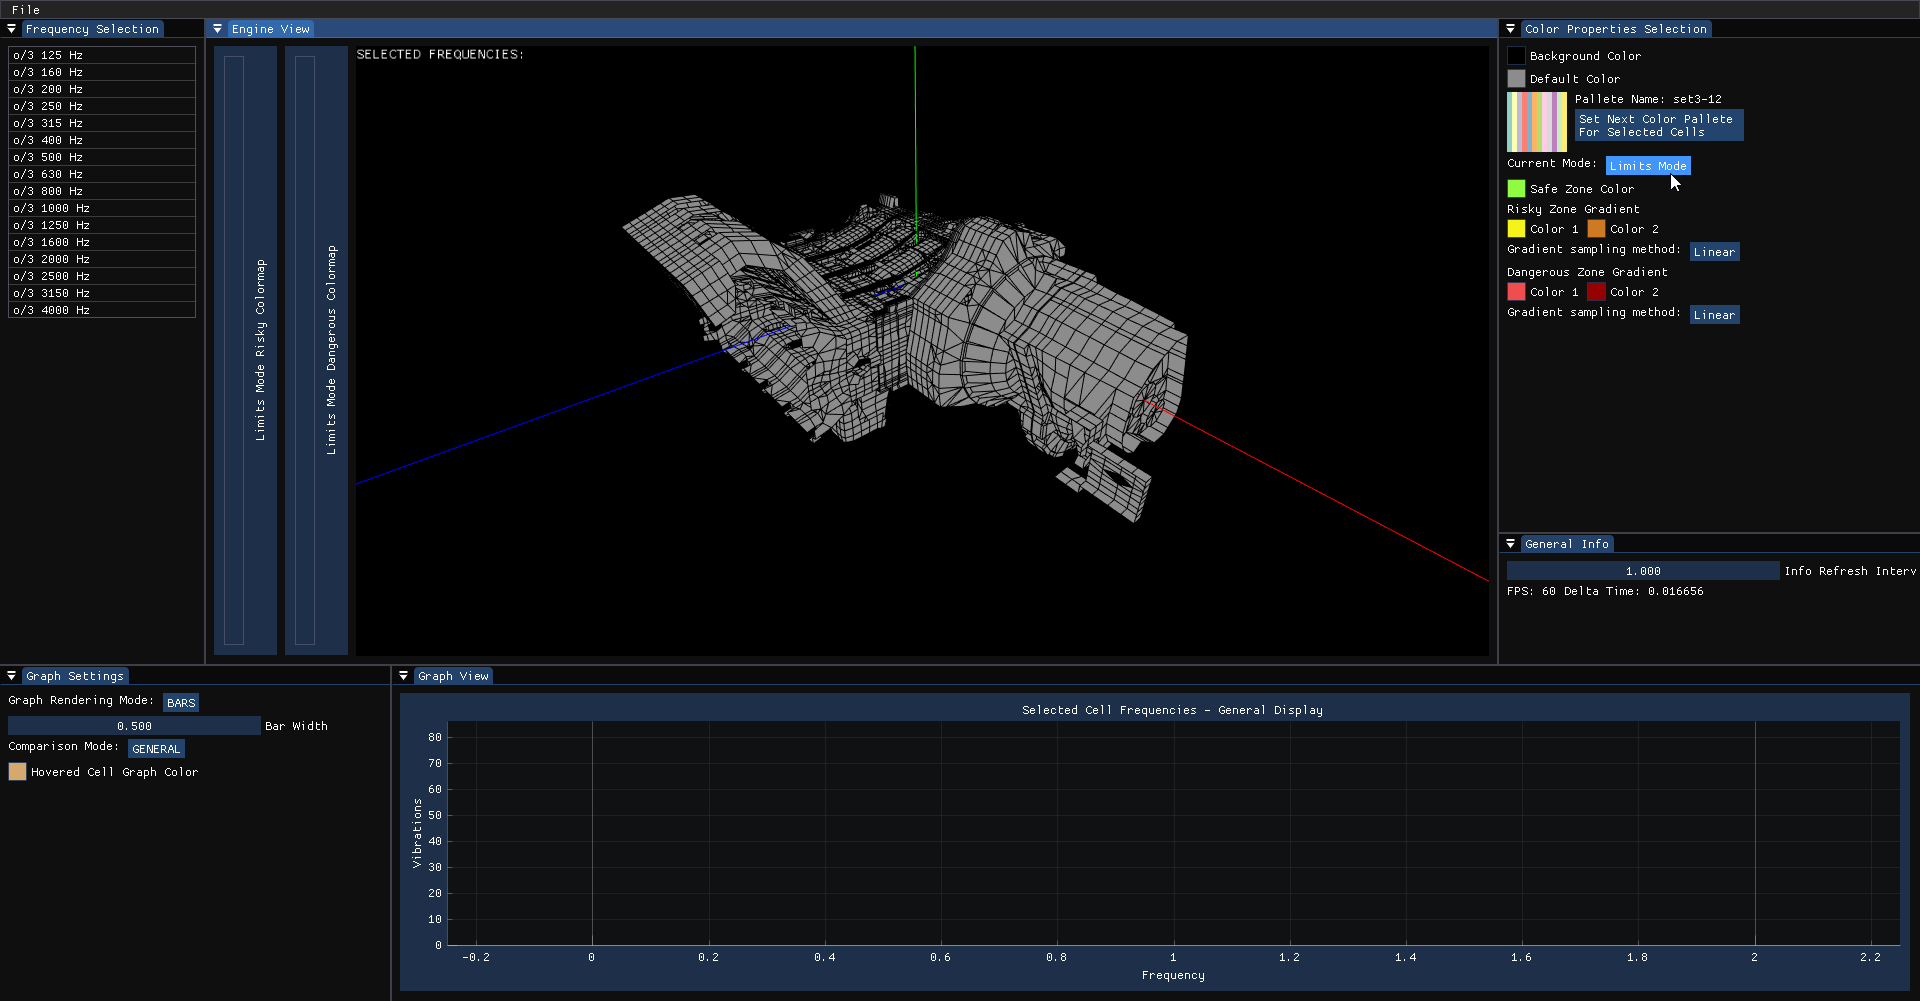
\includegraphics[width=\textwidth]{demonstration/limits_mode_opened.png}
    \caption{Početni izgled alata u analizi vibracija s preddefiniranim ograničenjima}
    \label{fig:limits-mode-switched}
\end{figure}

Na slici \ref{fig:limits-mode-frq-selected} se može vidjeti kako alat izgleda kada je u analizi vibracije s preddefiniranim ograničenjima odabrano nekoliko ponuđenih frekvencija vibriranja. U ovoj vrsti analize se također mogu mijenjati boje i metoda uzorkovanja gradijenta.

\begin{figure} [H]
	\centering
    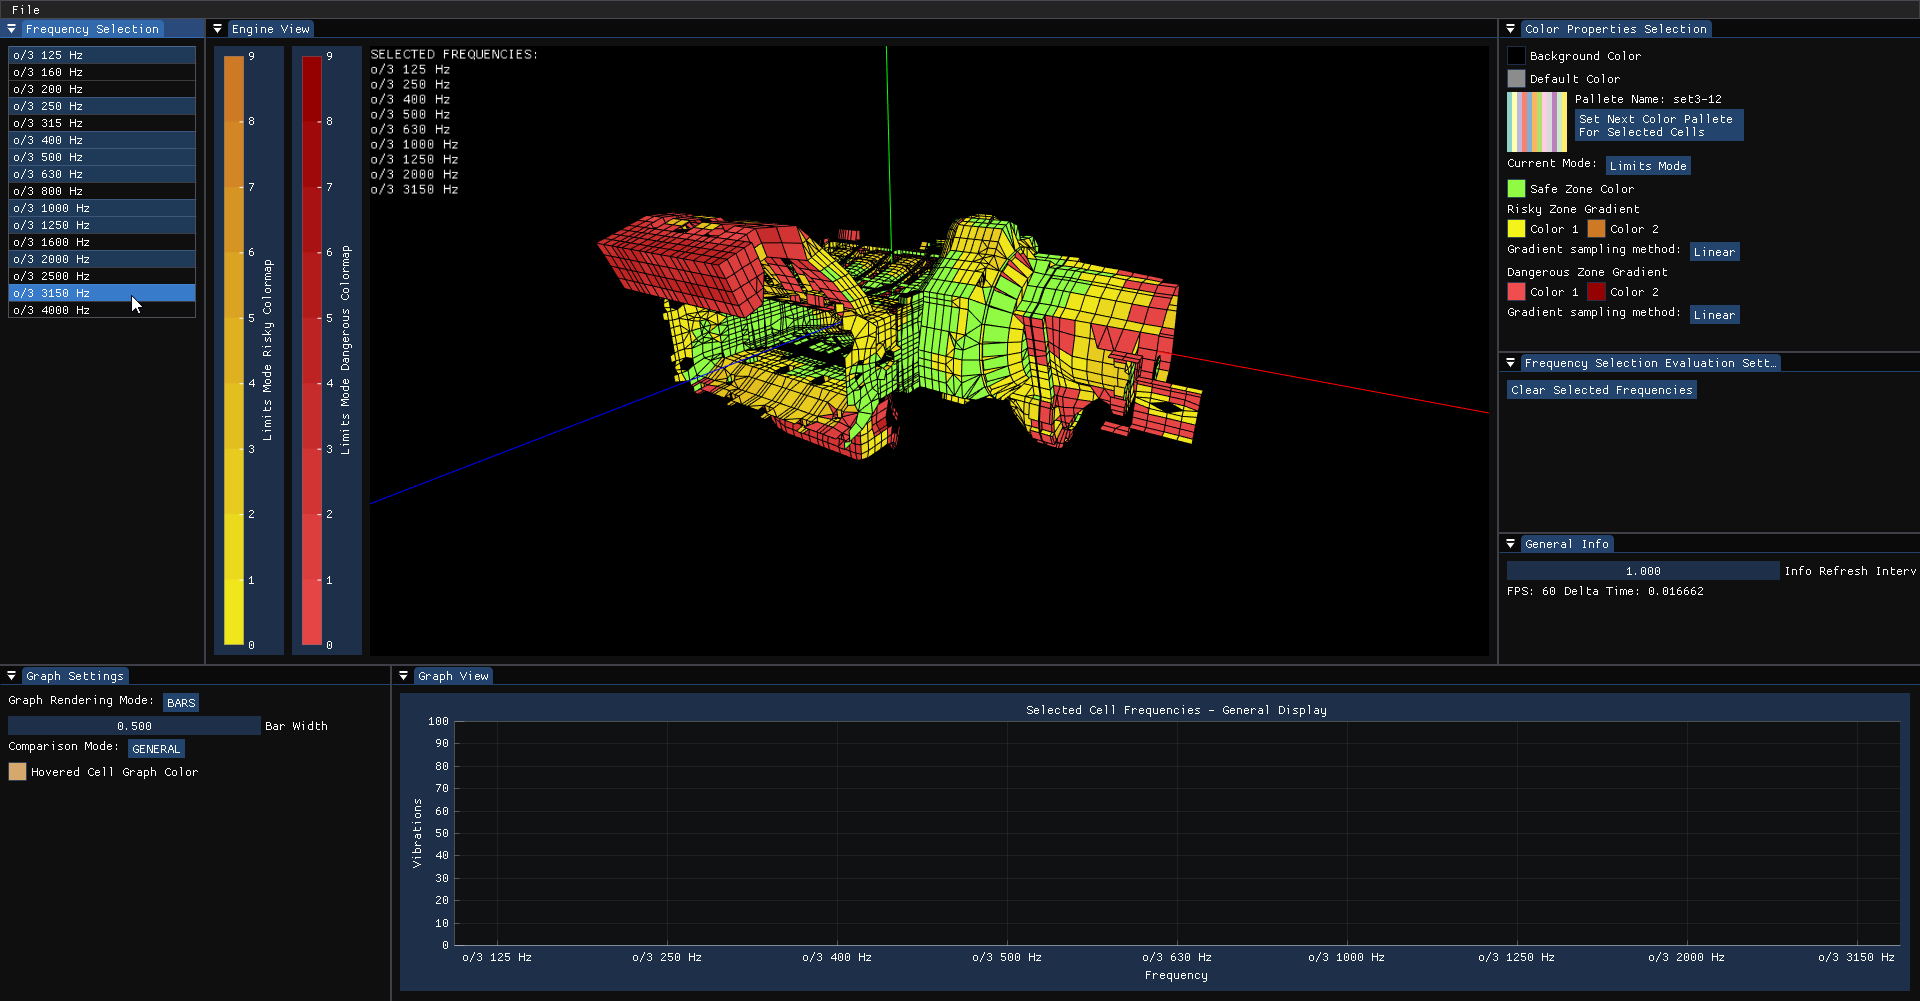
\includegraphics[width=\textwidth]{demonstration/limits_mode_frq_selected.png}
    \caption{Nekoliko odabranih frekvencija u analizi vibracija s preddefiniranim ograničenjima}
    \label{fig:limits-mode-frq-selected}
\end{figure}

\section{Uspoređivanje elemenata pomoću grafova}

Boje elemenata motora daju samo grubi pregled snage vibracije, ali ako korisnik želi detaljno analizirati kako se snaga vibracije elementa mijenja s obzirom na odabrane frekvencije, može koristiti 2D grafove koje alat nudi. Na slici \ref{fig:hovered-graph} se može vidjeti kako alat iscrtava 2D graf elementa iznad kojeg korisnik postavi pokazivač miša, a u tom grafu su prikazani podaci o snazi vibracije interesnog elementa pri svim odabranim frekvencijama. Kao što je u prijašnjim poglavljima već spomenuto, navedeni element se naziva "lebdeći" element, a boja grafa navedenog elementa se može mijenjati u postavkama grafa, koje se na spomenutoj slici nalaze u donjem lijevom kutu alata.

\begin{figure} [H]
	\centering
    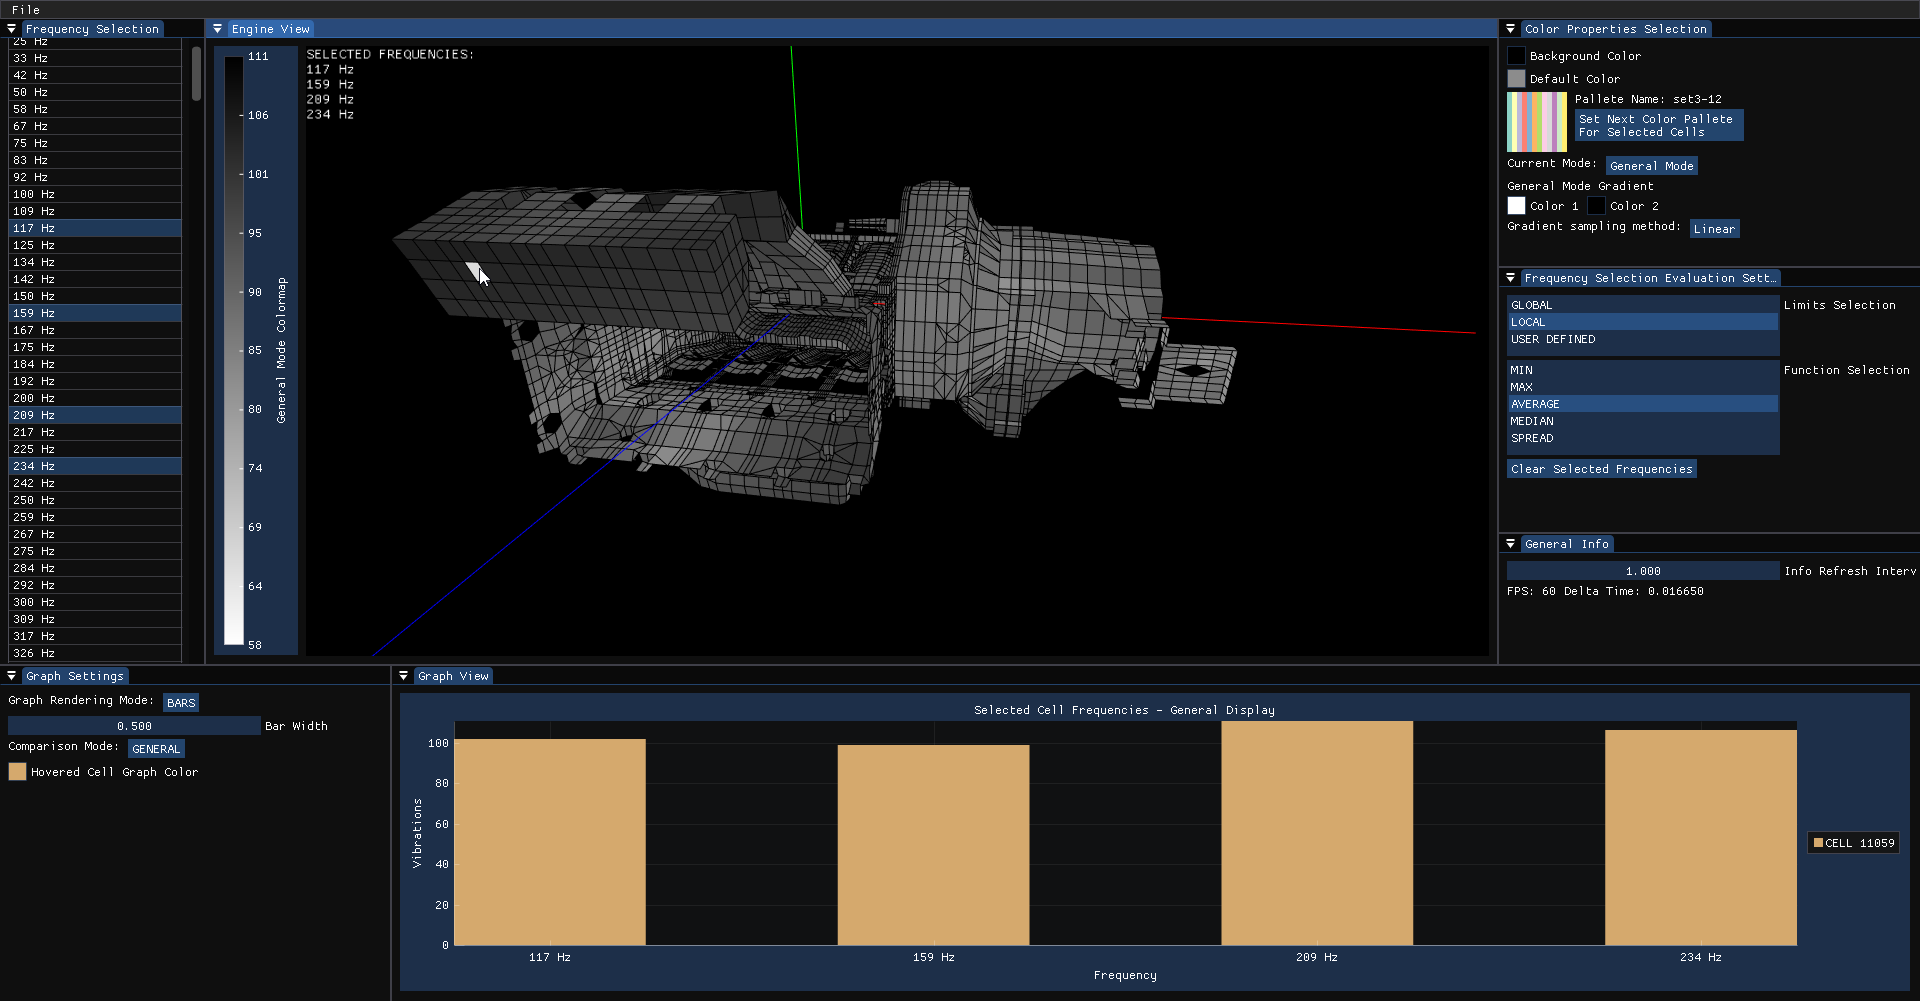
\includegraphics[width=\textwidth]{demonstration/cell_hovered.png}
    \caption{Graf "lebdećeg" elementa}
    \label{fig:hovered-graph}
\end{figure}

Korisnik može dodati trenutni "lebdeći" element u listu odabranih elemenata klikom na lijevu tipku miša, ali ako je "lebdeći" element već u listi odabranih elemenata, lijevi klik miša će ga maknuti iz liste. Odabiranjem elemenata, korisnik može detaljnije uspoređivati njihovu snagu vibracije s obzirom na odabrane frekvencije. Kao što je vidljivo sa slike \ref{fig:selected-cells-graphs}, odabrani elementi su obojani bojom iz trenutne palete, a grafovi im se konstantno nalaze u prikazu grafova. 

\begin{figure} [H]
	\centering
    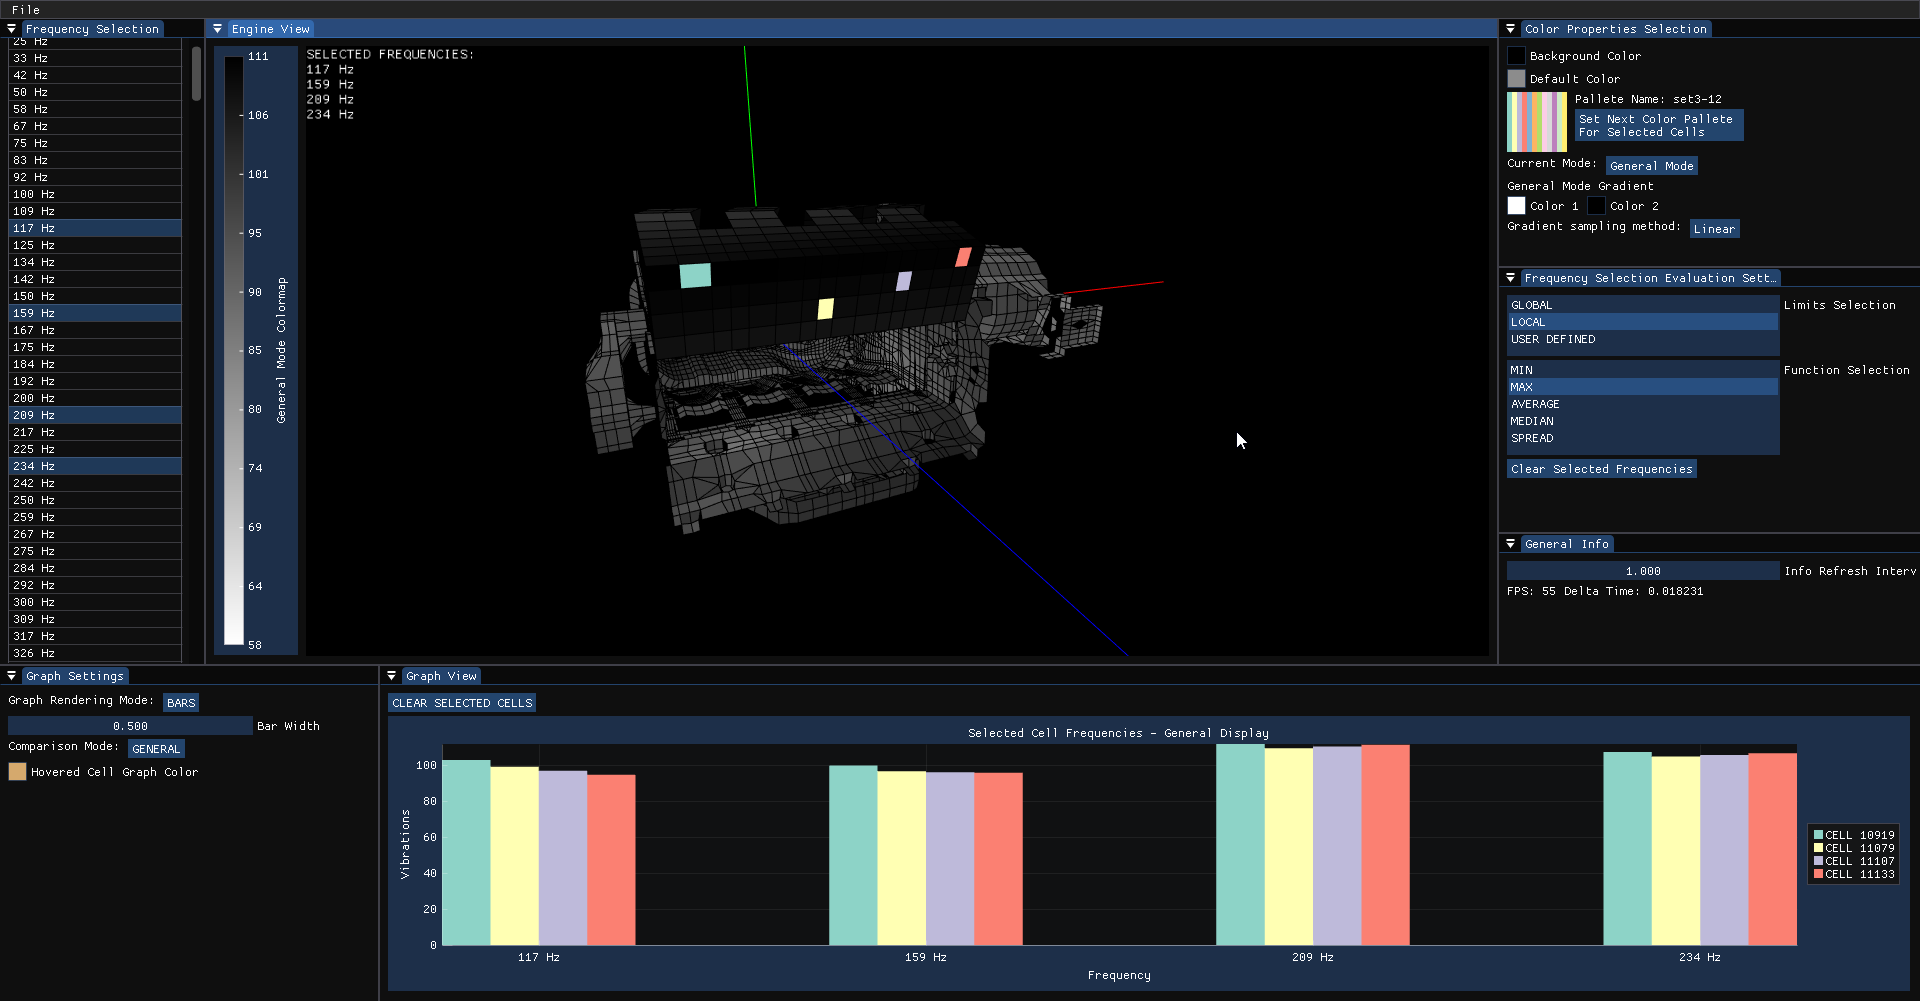
\includegraphics[width=\textwidth]{demonstration/selected_cells_max.png}
    \caption{Usporedba grafova odabranih elemenata}
    \label{fig:selected-cells-graphs}
\end{figure}

Važnost grafova pri uspoređivanju vibracija elemenata postaje očitija ako se usporede slike \ref{fig:selected-cells-graphs} i \ref{fig:hovered-cell-selected-cells} jer je promatrajući dijelove motora prikazane na tim slikama vidljivo kako su elementi na ta dva dijela motora slično obojani. Tek kada korisnik postavi pokazivač miša iznad jednog od elemenata sa slike \ref{fig:hovered-cell-selected-cells} postane očito kako se ne ponašaju ni približno slično.

\begin{figure} [H]
	\centering
    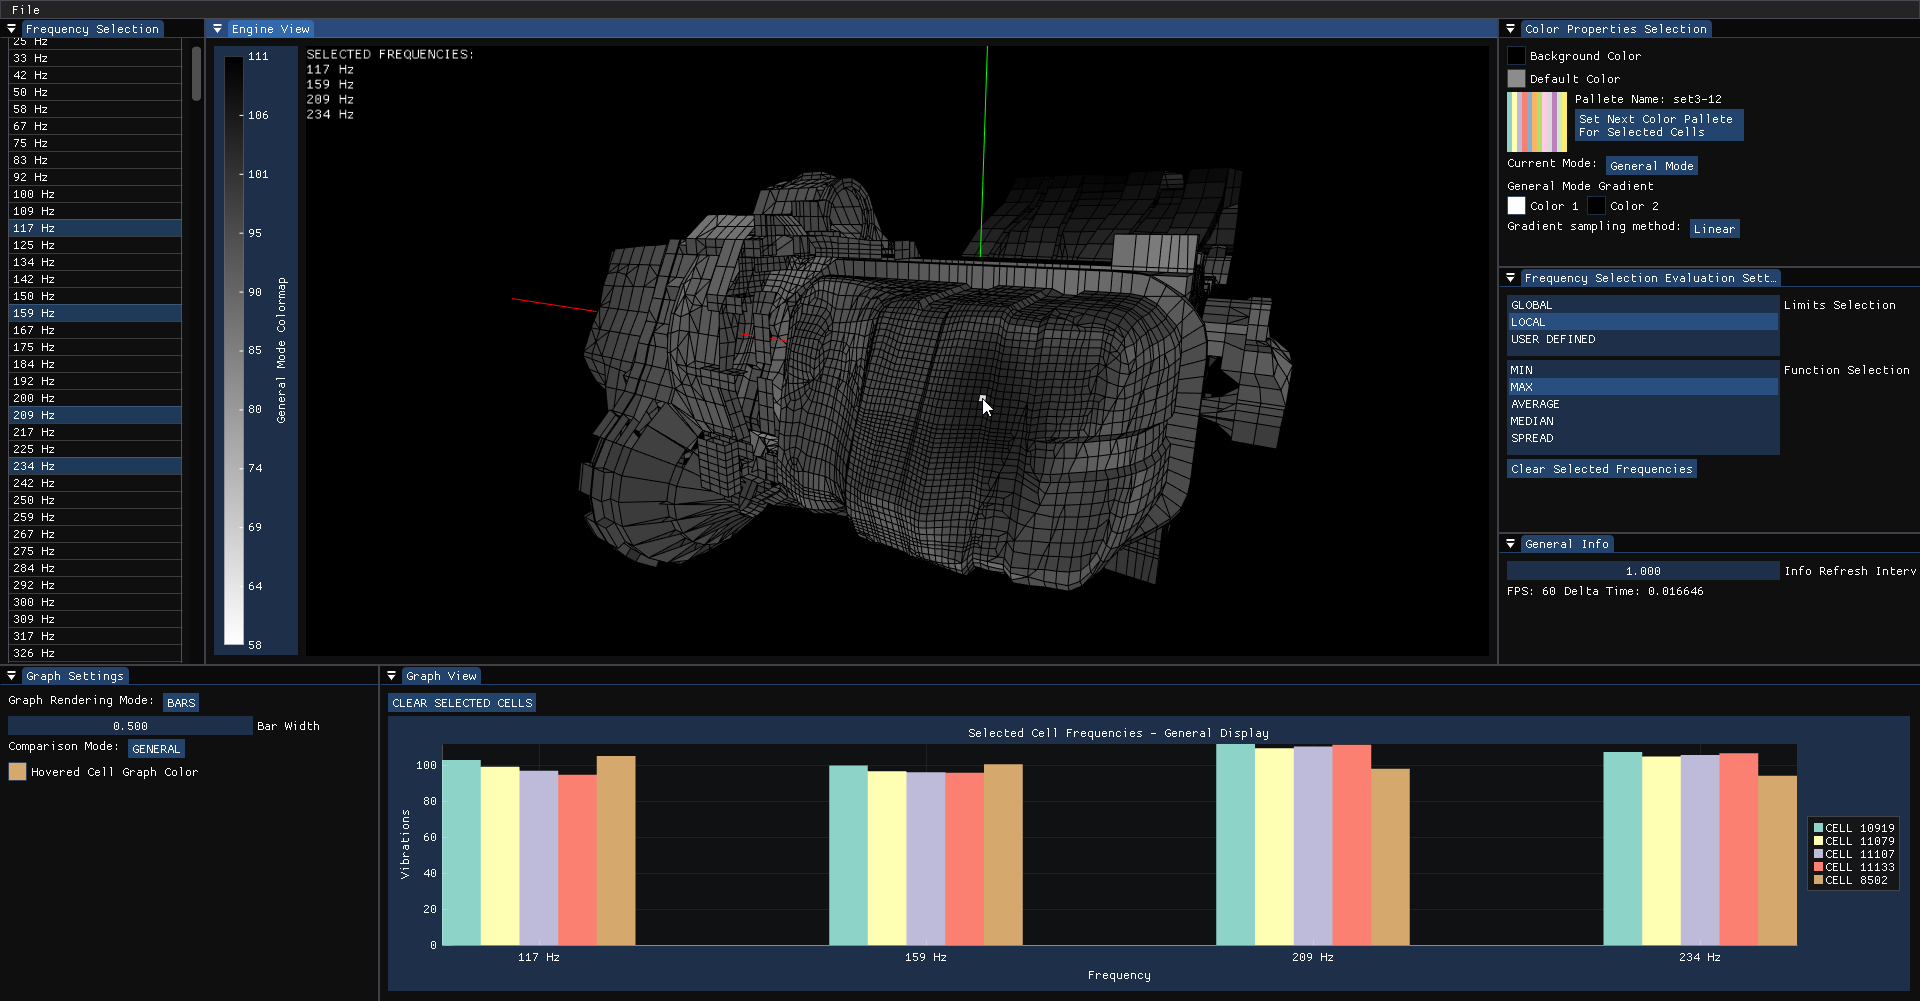
\includegraphics[width=\textwidth]{demonstration/hovered_cell_max.png}
    \caption{"Lebdeći" element koji ima približan maksimum kao i odabrani elementi na drugom dijelu motora}
    \label{fig:hovered-cell-selected-cells}
\end{figure}

Korisnik može promijeniti način usporedbe klikom na gumb koji nosi ime trenutnog načina usporedbe (u postavkama grafa). Slike \ref{fig:subplots-graph-comp} i \ref{fig:relative-graph-comp} prikazuju dodatne moguće načine na koje korisnik može usporediti odabrane elemente.


\begin{figure} [H]
	\centering
    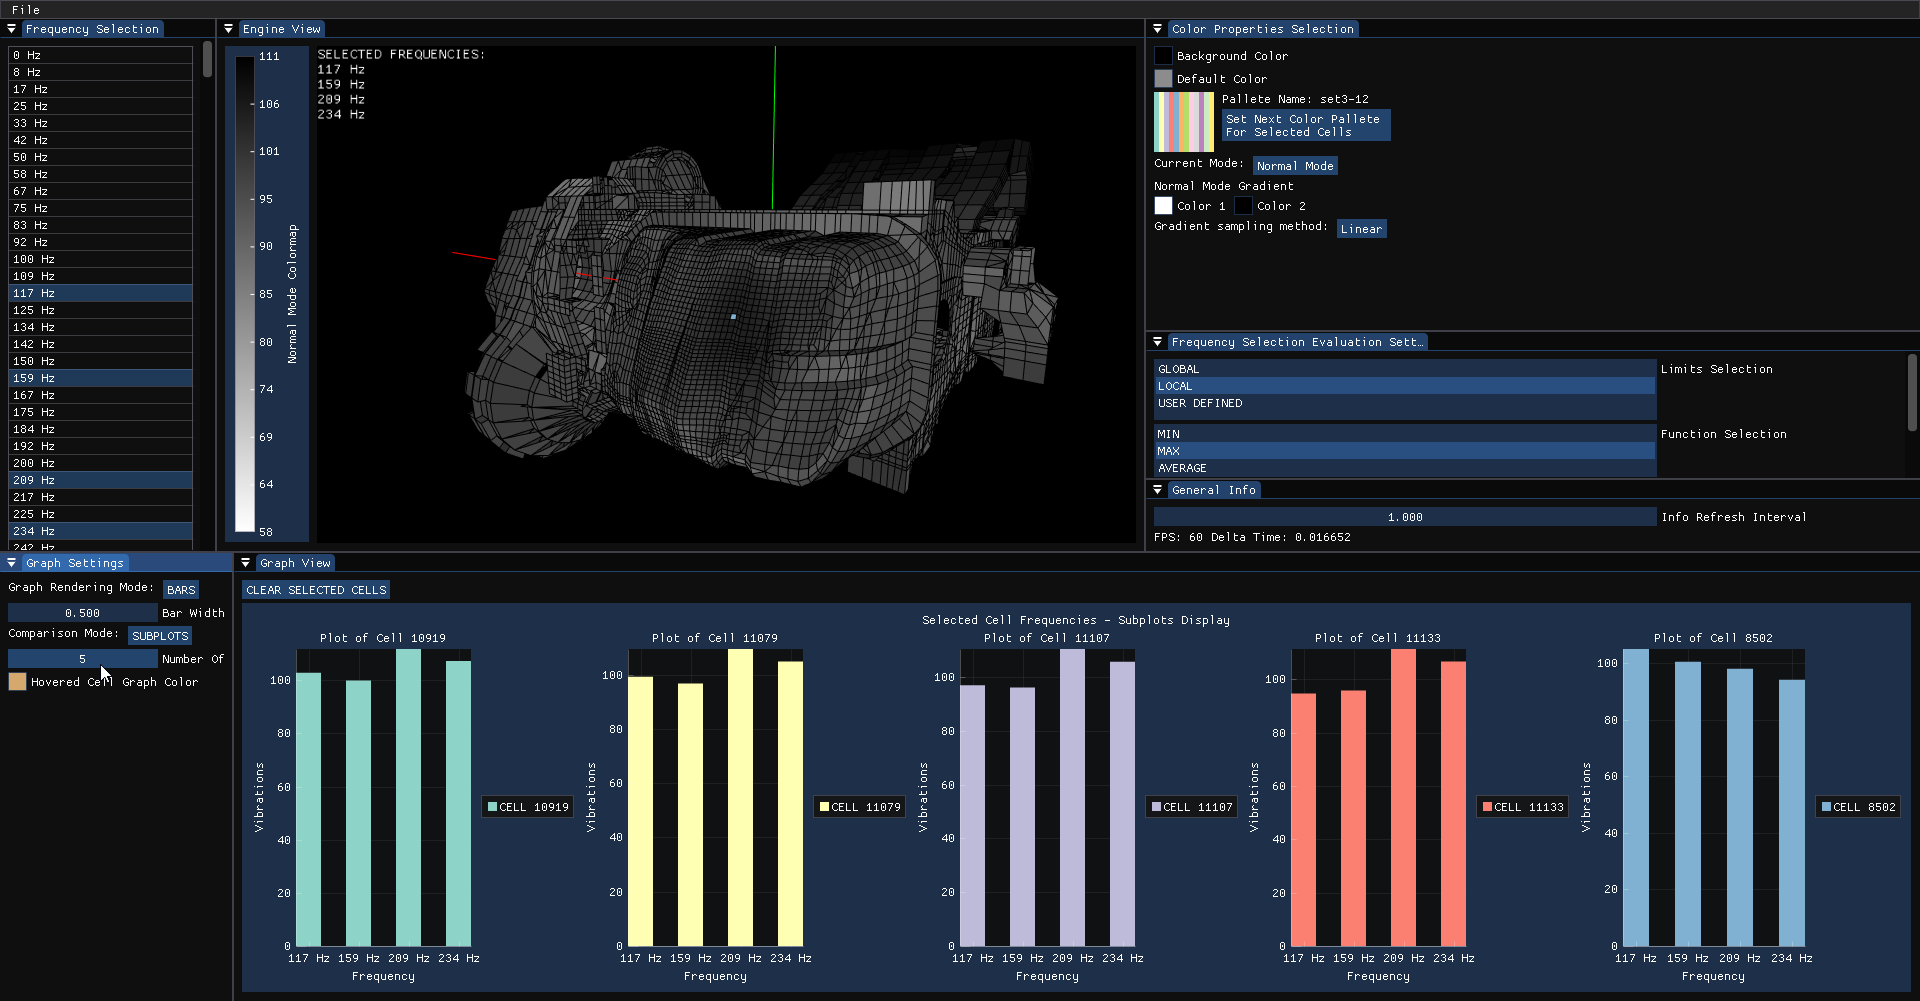
\includegraphics[width=\textwidth]{demonstration/selected_cell_subplots.png}
    \caption{Prikaz grafova u načinu usporedbe s višestrukim prikazima}
    \label{fig:subplots-graph-comp}
\end{figure}

\begin{figure} [H]
	\centering
    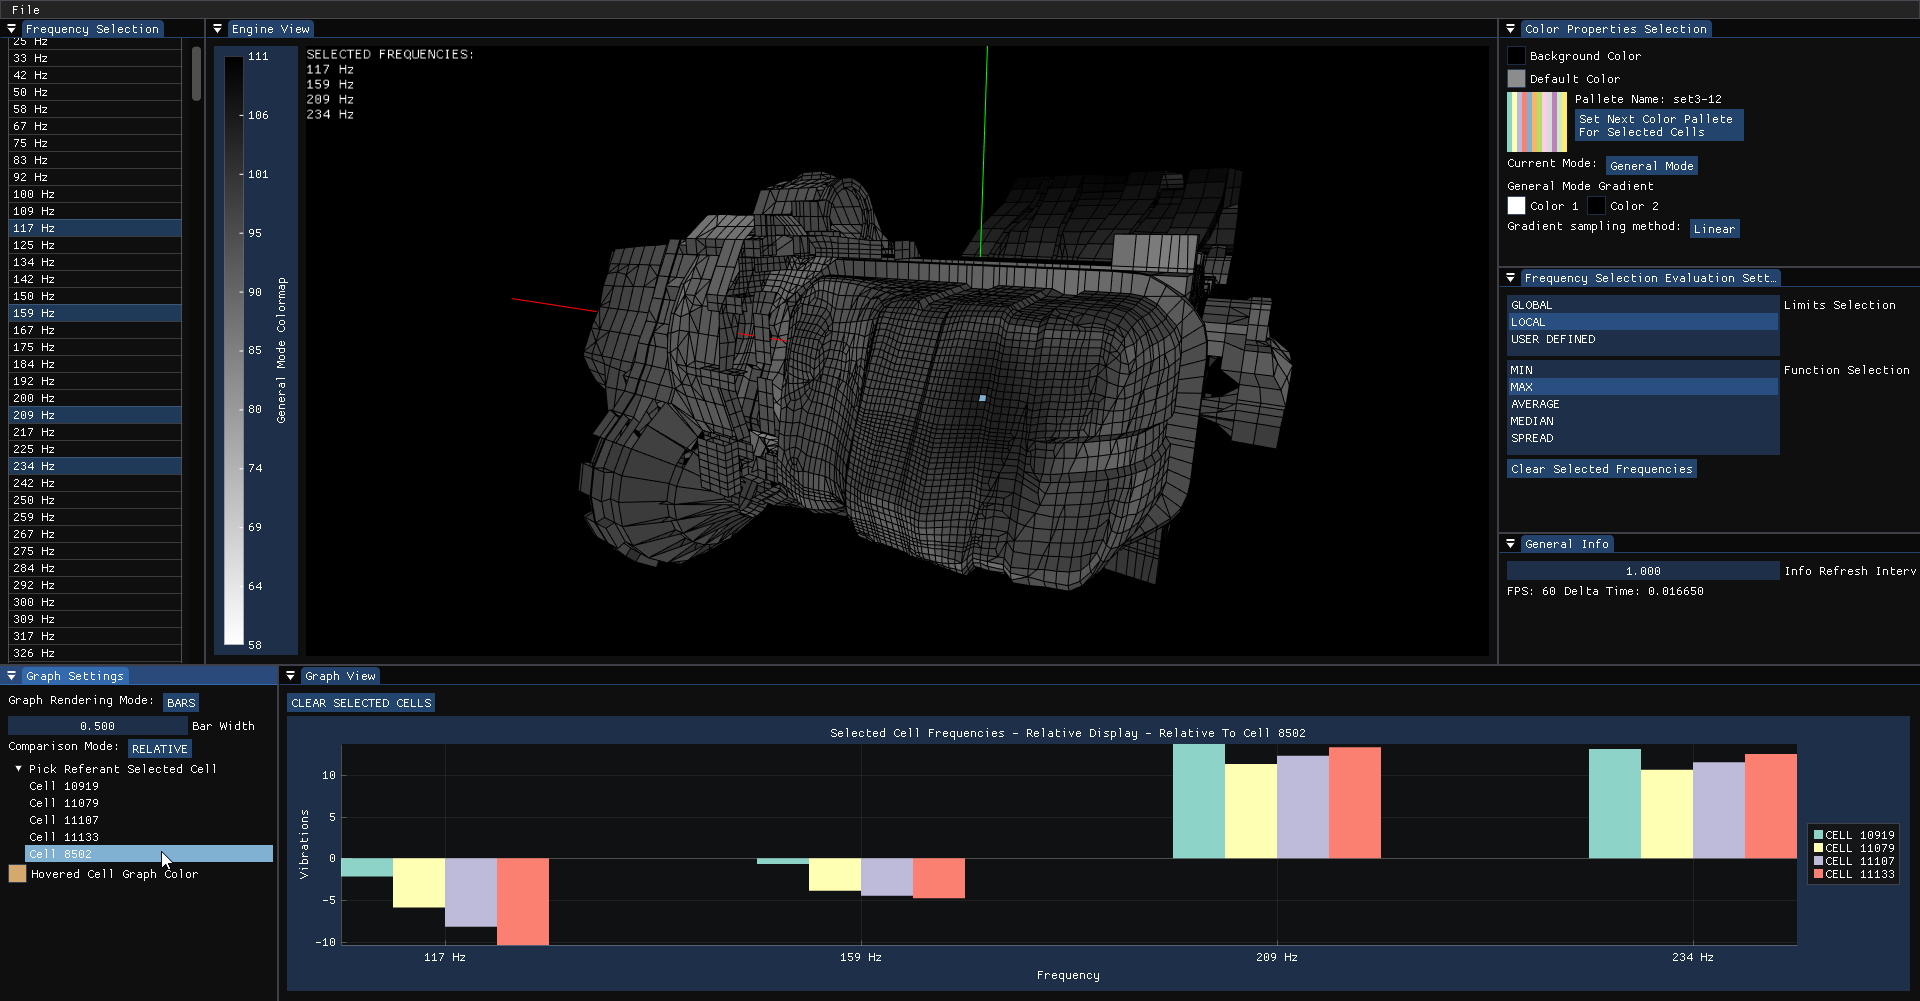
\includegraphics[width=\textwidth]{demonstration/selected_cell_relative.png}
    \caption{Prikaz grafova u relativnom načinu usporedbe}
    \label{fig:relative-graph-comp}
\end{figure}

\chapter{Zaključak}

Alat razvijen u sklopu ovog rada uvelike poboljšava mogućnosti uspoređivanja snaga vibracija dijelova motora na različitim frekvencijama vibriranja. U sklopu alata se korisniku nude dvije vrste analize vibracija koje nude različite poglede na iste podatke koji opisuju vibriranje motora. Općenita analiza vibracija omogućuje odabir više frekvencija na temelju kojih će se određivati boje dijelova motora, ali omogućuje i odabir funkcije pomoću koje će se niz podataka o snazi vibracije dijelova motora na odabranim frekvencijama evaluirati u konačni podatak. Analiza vibracija s preddefiniranim ograničenjima korisniku pruža mogućnost definiranja ograničenja na temelju kojih će se elementi motora svrstati u tri klase s obzirom na snagu vibriranja pri odabranim frekvencijama vibracije motora. Osim vizualizacije podataka pomoću 3D modela motora, alat prikazuje podatke korisniku i pomoću 2D grafova za koje su implementirana tri načina uspoređivanja. Spomenuti grafovi nisu zamjena za prikaz podataka na modelu motora, već su nadopuna jer korisniku pružaju mogućnost detaljnije i preciznije analize podataka vezanih za odabrane frekvencije i elemente.\\

Za alat bi bilo dobro kad bi se nastavio razvijati u smjeru pokrivanja funkcionalnosti iz rada \citep{matkovic2021getting}, prvenstveno dodataka poput interaktivne selekcije i vezanih višestrukih prikaza jer bi navedeni dodaci uvelike doprinijeli jednostavnosti korištenja alata. Ručno spremanje postavki alata bi također bilo koristan dodatkak, s time da bi te postavke uključivale ne samo raspored prozora, već i odabrane gradijente, boje i ostale faktore koje korisnik može mijenjati u alatu. No, na kraju bi najvažnije bilo dodatno evaluirati alat u suradnji sa stručnjacima koji bi ga koristili, kako bi se dobile povratne informacije o unaprjeđivanju postojećih i implementaciji novih mogućnosti koje bi stručnjacima bile od velike koristi.

\bibliography{literatura}
\bibliographystyle{fer}

\appendix

\chapter{Sustav događaja i signala} \label{appendix:event-signal-system}

Sustav događaja i signala je razvijen u sklopu ovog rada kako bi se olakšalo korištenje obrasca Promatrač. Sustav je implementiran pomoću klasa \textit{Event} i  \textit{Signal} čiji je k\^{o}d prikazan u nastavku.\\

\begin{lstlisting}[caption={Klasa \textit{Event}},captionpos=b]
template <typename T>
class Event {
private:
	std::vector<std::function<void(T)>> m_listeners;
public:
	void add_listener(std::function<void(T)> listener) {
	 m_listeners.push_back(listener); 
	}
	
	template <typename L>
	void add_member_listener(void(L::*m)(T), L* l) {
	 add_listener(std::bind(m, l, std::placeholders::_1)); 
	}
	
	void invoke(T var) {
	for (auto& l : m_listeners)
		l(var);
	}
};
\end{lstlisting}

\begin{lstlisting}[caption={Klasa \textit{Signal}},captionpos=b]
class Signal {
private:
	std::vector<std::function<void()>> m_listeners;
public:
	void add_listener(std::function<void()> listener) { m_listeners.push_back(listener); }

	template <typename L>
	void add_member_listener(void(L::* m)(), L* l) { add_listener(std::bind(m, l)); }

	void invoke() {
	for (auto& l : m_listeners)
		l();
	}
};
\end{lstlisting}
\
\\

Obje klase funkcioniraju na način da im se u listu "promatrača" dodaju funkcije koje instanca ovih klasa zatim pozove kada se pozove članska funkcija \textit{invoke}. Kada se pozove spomenuta funkcija nad objektom klase \textit{Event}, potrebno joj je predati argument koji će ona proslijediti svim funkcijama koje su "pretplaćene" na taj događaj. S druge strane, funkcija \textit{invoke} klase \textit{Signal} ne prima argumente jer sve funkcije koje se "pretplaćuju" na instance ove klase također ne primaju argumente.\\

U obje navedene klase postoje dvije različite funkcije koje služe za registriranje funkcija koje se pozivaju pri aktivaciji događaja: \textit{add\_listener} i \textit{add\_member\_listener}. Funkcija \textit{add\_member\_listener} služi za "registriranje" članskih funkcija jer one zahtijevaju dodatno definiranje pokazivača na objekt čiju se člansku funkciju poziva. Funkcija \textit{add\_listener} se koristi za dodavanje svih ostalih funkcija.

\begin{sazetak}
Osiguravanje minimalne razine buke motora je jedan od ključnih zadataka inženjera pri projektiranju motora, stoga im je iznimno važno održati vibriranje motora prilikom rada na što nižoj razini jer vibracija motora izravno utječe na buku koju motor proizvodi. NVH \engl{Noise, Vibration, Harshness} simulacije pružaju jednostavan način provjere snage vibracija pojedinih dijelova motora u fazi projektiranja. No, računske simulacije ove vrste nerijetko proizvode podatke koje se ne može jednostavno analizirati, pa alati za vizualizaciju uvelike pomažu stručnjacima kod stvaranja ispravne predodžbe o izračunatim podacima. Ovaj rad opisuje izradu alata za vizualizaciju podataka dobivenih iz NVH simulacije pomoću 3D modela motora i 2D grafova. Fokus predstavljenog alata je omogućavanje jednostavnijeg načina uspoređivanja vibracije dijelova motora s obzirom na odabrane frekvencije.

\kljucnerijeci{vizualizacija, 3D, NVH podaci, C++, OpenGL}
\end{sazetak}

\engtitle{3D Interactive Visualization of Vibration Simulation}
\begin{abstract}

Minimizing engine noise presents an important task when designing an engine, so it is of utmost importance to keep the engine vibration strength at the lowest possible level since it directly affects the noise level produced by the engine. NVH (Noise, Vibration, Harshness) simulations provide an easy way to check the vibration strength of individual engine parts at the design stage. However, computational simulations of this kind often produce data that is hard to analyze, so visualization tools help significantly by presenting the calculated data intuitively and understandably. This thesis describes the development of an application for visualizing data obtained from NVH simulation using a 3D engine model and 2D graphs. The focus of the presented tool is to enable a simpler way of comparing the vibration of engine parts with respect to selected frequencies.

\keywords{visualization, 3D, NVH data, C++, OpenGL}
\end{abstract}

\end{document}
